\documentclass[10pt]{article}
\usepackage{commands}
\usepackage{slashed}
\pgfplotsset{compat=1.18}

\begin{document}
\begin{tcolorbox}
  \begin{center}
  \begin{Large}
    \textbf{PHYS 444 (Quantum Field Theory II) Notes} \\
    \vspace{5pt}
  \end{Large}
  \begin{large}
        Rio Weil \\
\vspace{5pt}
    \emph{This document was typeset on \today}
  \end{large}
  \end{center}
\end{tcolorbox}

\begin{center}
  \textbf{Introduction:}

  This is a set of lecture notes taken from UChicago's PHYS 444 (Quantum Field Theory II), taught by Luca Delecretaz. Topics covered include representations of the Lorentz group, Quantizing the Dirac field, Path integrals for fermions, Interacting fermions, Relativistic electrodynamics, Path integral for gauge fields, Radiative corrections, The electron magnetic dipole moment, Renormalization for QED, LSZ for fermions/photons, QED scattering, Soft divergences in QED, Non-Abelian gauge fields, QCD and quantizing Yang-Mills, Wilson line and loop operators.

\end{center}
\addtocontents{toc}{\protect\hypertarget{toc}{}}
\tableofcontents

\newpage
\section{Fermions - Representations of Lorentz}

\subsection{Introduction}
In QFTI we explored scalar QFT deeply; both perturbatively and non-perturbatively. We looked at the path integral formalism, renormalization, and scattering. But the elephant in the room is we did this all with scalar fields, and most particles in the universe... are not. They transform with different representations of the Lorentz group; the scalar field is simply the simplest one. 

In this course, we will look at fermions; they are qualitatively different due to Pauli exclusion and will lead to new physics. Building on this, we can build Lagrangians in 3+1 dimensions with dimensionless couplings, and moreover different kinds of dimensionless couplings. This will lead us into quantum electrodynamics eventually; but let's start with a discussion of fermions.

\subsection{Representations of the Lorentz group; scalar and vector representations}
Recall the Lorentz group $O(1, 3)$; it consists of all transformations that leaves spacetime distance invariant, i.e. all transformations:
\begin{equation}
    x^\mu \to \Lambda^\mu_{\nu}x^\nu
\end{equation}
such that:
\begin{equation}
    \Lambda^{\mu}_\alpha\Lambda^\nu_\beta \eta^{\alpha\beta} = \eta^{\mu\nu}
\end{equation}
with $\eta = \text{diag}(-1, 1, 1, 1)$ the Minkowski metric.

We have already studied its simplest representation on fields, the scalar field:
\begin{equation}
    \phi(x) \to \phi'(x') = \phi(x)
\end{equation}
This is not a trivial representation (the field does transform), but in a way that is completely absorbed by the transformation of the coordinates.

This is realized on Hilbert space/quantum fields $\hat{\phi}$ by a unitary operator:
\begin{equation}
    \hat{\phi}(x) \to U(\Lambda)^{-1}\hat{\phi}(x)U(\Lambda) = \hat{\phi}(\Lambda^{-1}x).
\end{equation}

Out of scalar fields, we could build composite objects that transform in potentially other representations. The simplest example is taking higher powers of the field, $[\phi(x)]^n$ still transforms as a scalar. But, consider $A_\mu = \p_{x^\mu}\phi(x)$; this transforms in a 4-vector representation:
\begin{equation}
    A_\mu(x) \equiv \p_{x^\mu}\phi(x) \to U(\Lambda)^{-1}\p_{x^\mu}\phi(x)U(\Lambda) = \p_{x^\mu}\phi(\Lambda^{-1}x) = \p_{x^\mu}\phi(\bar{x}) = \frac{\partial \bar{x}^\nu}{\partial \bar{x}^\mu}\p_{x^\mu}\phi(\bar{x}) = \Lambda^{\sp \nu}_{\mu}\p_{\bar{x}^\nu}\phi(\bar{x})
\end{equation} 
Where in the last equality we use that new coordinates are linearly related to the old coordinates, with:
\begin{equation}
    \frac{\partial \bar{x}^\nu}{\partial x^\mu} = (\Lambda^{-1})^{\mu}_{\sp\nu} = \Lambda^{\sp \nu}_{\mu}
\end{equation}
And thus:
\begin{equation}
    A_\mu(x) \to \Lambda^{\sp \nu}_{\mu}A_\nu(\bar{x})
\end{equation}
or:
\begin{equation}
    U(\Lambda)^{-1}A_\mu(x)U(\Lambda) = \Lambda_{\mu}^{\sp\nu} A_\nu(\Lambda^{-1}x)
\end{equation}
Under the spatial rotation subgroup $O(3) \subset O(1, 3)$, this splits into a scalar part for the time component $A_0$ and a 3-vector part for the spatial components $A_i$.

The photon is a particle in this 4-vector representation of Lorentz. In that case, $A_\mu$ is the (fundamental) group field in Maxwell's equations, with the field:
\begin{equation}
    F_{\mu\nu} = \p_\mu A_\nu - \p_\nu A_\mu
\end{equation}
or:
\begin{equation}
    E_i = \p_0 A_i - \p_i A_0, \quad B_i = \e_{ijk}\p_jA_k
\end{equation}

\subsection{General Representation of Lorentz}
We will come back to the photon later in the course, but let us turn to the question of building a general representation of the Lorentz group. To this end, we study its algebra. It contains the generator of rotations $J_i$:
\begin{equation}
    [J_i, J_j] = i\e_{ijk}J_k \quad \text{($\mathfrak{su}(2)$ algebra)}
\end{equation}
which forms a subalgebra. It also contains the generator of boosts $K_i$:
\begin{equation}
    [K_i, K_j] = -i\e_{ijk}J_k
\end{equation}
\begin{equation}
    [J_i, K_j]= i\e_{ijk}K_k.
\end{equation}
but the $K_i$ do not form a closed subalgebra. Rotations and boosts together form the full Lorentz algebra, which we derived last quarter through the study of infinitesimal transformations.

We consider the following linear combinations of generators:
\begin{equation}
    J_i^\pm = \frac{1}{2}(J_i \pm iK_i).
\end{equation}
It can be easily checked that the $J^+$s form a closed subalgebra:
\begin{equation}
    [J_i^+, J_j^+] = \frac{1}{4}[J_i + iK_i, J_j + iK_j] = \frac{1}{2}(i\e_{ijk}J_k - \e_{ijk}K_k) = i\e_{ijk}\frac{1}{2}(J_k + iK_k) = i\e_{ijk}J^+
\end{equation}
Moreover the $J^+$s commute with the $J^-$s:
\begin{equation}
    [J_i^+, J_j^-] = \frac{1}{4}[J_i + iK_i, J_j - iK_j] = 0.
\end{equation}
and the $J^-$s have the same commutation relation with each other as the $J^+$s:
\begin{equation}
    [J_i^-, J_j^-] = i\e_{ijk}J^-_k
\end{equation}
Thus, we conclude that the Lorentz algebra is just 2 commuting $\mathfrak{su}(2)$ algebras! We thus conclude that:
\begin{equation}
    \mathfrak{so}(1, 3) = \mathfrak{su}(2) \oplus \mathfrak{su}(2)
\end{equation}
The usual representation of $\mathfrak{su}(2)$ is labelled by a half-integer, and thus the irreducible representations of the Lorentz group are thus labelled by two half-integers $(j^-, j^+)$, with:
\begin{equation}
    j^\pm = 0, \frac{1}{2}, 1, \frac{3}{2}, \ldots
\end{equation}
Thus a general field $\Psi_{ab}(x)$ has two indices, with $a = 1, \ldots, 2j_- + 1$ and $b = 1, \ldots, 2j_+ + 1$.

\subsection{Examples of Lorentz Representations}
For a scalar field, we have the $(0, 0)$ representation. In this case, the indices $a, b$ run from 1 to 1 so we just omit the indices and write $\phi(x)$.

For rotations, we have $J_i = J^+_i + J^-_i$. The $(j^-, j^+)$ irrep (irreducible representation) of Lorentz therefore decomposes into spin:
\begin{equation}
    \abs{j^- - j^+}, \abs{j^- - j^+} + 1, \ldots, j^- + j^+
\end{equation}
under rotations.

Let's look at a slightly more interesting example. What is the 4-vector representation? A first guess is that a vector looks like spin-1, so we might put $(1, 0)$; but this doesn't work because under rotation it doesn't split into a scalar rotation $A_0$ and a 3-vector $A_i$. Thus, the correct representation turns out to be $(\frac{1}{2}, \frac{1}{2})$. Under spatial rotation, this decomposed into a spin 0 $(A_0)$ and spin 1 $(A_i)$ piece, which is what we need.

This skipped one representation though! What about $(\frac{1}{2}, 0)$ or $(0, \frac{1}{2})$ (these are the smallest non-scalar irreps)? Well, first note that these reps are related by a parity $\v{x} \to -\v{x}$, as under this reflection angular momentum is invariant and boosts are flipped, i.e.:
\begin{equation}
    \v{J} \to \v{J}, \quad \v{K} \to -\v{K}
\end{equation}
and so:
\begin{equation}
    J_i^\pm \to J_i^\mp
\end{equation}
Hence a $(\frac{1}{2}, 0)$ particle cannot be parity invariant on its own. We will later study these in ``chiral'' theories. This rep is the left or right handed Weyl (or Majorana\footnote{in 3+1 dimensions they coincide, but in other dimensions they differ, hence the two different names.}) spinor.

\subsection{Properties of the Weyl spinor}

We're in the USA, so let's pick the right-handed representation $(0, \frac{1}{2})$. In this rep:
\begin{equation}
    J_+^i = \frac{1}{2}\sigma^i
\end{equation}
which satisfy:
\begin{equation}
    [J_+^i, J_+^j] = i\e_{ijk}J_k
\end{equation}
which is a 2-d rep of $\mathfrak{su}(2)_+$. The minus matrices are trivial, with:
\begin{equation}
    J_-^i = 0.
\end{equation}
giving the 1-d rep of $\mathfrak{su}(2)_-$. These two objects act on different spaces (one on the right, one on the left index). If we want to see them as the representation of the entire group $SU(2) \times SU(2)$, we can write:
\begin{equation}
    J_i^+ = \II \otimes \frac{1}{2}\sigma_i, \quad J_i^- = 0 \otimes \II
\end{equation}
From this we can also get the generators of rotations and boosts:
\begin{equation}
    J_i = J_i^+ + J_i^- = \frac{1}{2}\sigma_i
\end{equation}
\begin{equation}
    K_i = \frac{1}{i}(J_i^+ - J_i^-) = -\frac{i}{2}\sigma_i
\end{equation}
We therefore have a 2-d representation of Lorentz $(0, \frac{1}{2})$ on fields $\psi_R = \m{\psi_1 \\ \psi_2}$. For a Lorentz transformation $\Lambda$ of angles $\theta_i$ and rapidities $\eta_i$, i.e. $\Lambda = e^{i(\theta^i J_i + \eta^i K_i)}$, we have the fields transform as:
\begin{equation}
    U(\Lambda)^{-1}\psi_R(x)U(\Lambda) = e^{\frac{i}{2}(\theta_i - i\eta^i)\sigma_i}\psi_R(\Lambda^{-1}x)
\end{equation}
note that the rotation part is unitary but the boost part is not. Because the boost generators are related to the $J^\pm$s via an $i$, in any representation it will be anti-unitary:
\begin{equation}
    K_i^\dagger = -K_i
\end{equation}
but do not confuse this with the full transformation on the Hilbert space, which is always unitary. Another comment; this implies that $\psi_R$ must be complex, as the transformation does not take real to real. In fact, the anti-unitarity of the $K_i$s implies that $\psi_R^*$ transforms in the parity flipped $(\frac{1}{2}, 0)$ representation.

Another interesting feature of this representation is that under a $2\pi$ rotation, say, around the $\zhat$ axis (so $\theta^z = 2\pi$), the field transforms to:
\begin{equation}
    \psi_R'(x) = e^{\frac{i}{2}(2\pi \sigma_z)}\psi_R(\Lambda^{-1}x) = e^{i\pi \sigma_z}\psi_R(x) = -\psi_R(x)
\end{equation}
note that $\Lambda^{-1}x = x$ as the coordinate comes back to itself. So, in scalar field theory a $2\pi$ rotation leaves the field invariant. But here, the field does \emph{not} transform back into itself due to the negative sign out front. This is a first hint of the spin-statistics theorem, which we will soon discuss; but this theorem will tell us that the particles must be fermionic. The statistics are tied to the representation of the Lorentz group.

\subsection{Building a Lagrangian for the Weyl spinor}
Let us start by building a quadratic/Gaussian Lagrangian for $\psi_R$. We could try tensoring $\psi^*_{Ra}\psi_{Rb}$. Since $\psi_R \in (0, \frac{1}{2})$ and $\psi_R^* \in (\frac{1}{2}, 0)$, from group theory:
\begin{equation}
    \psi^*_{Ra}\psi_{Rb} \in (0, \frac{1}{2}) \otimes (\frac{1}{2}, 0) = (0 \otimes \frac{1}{2}, \frac{1}{2}\otimes 0) = (\frac{1}{2}, \frac{1}{2})
\end{equation}
which as we discussed previously, transforms like a 4-vector. But it doesn't look like one... it looks like a $2\times 2$ matrix. But there should be a way to map it to a 4-vector. What are the possible bilinears we can build? Well, we can consider:
\begin{equation}
    A_0 = \psi_R^\dagger \psi_R
\end{equation}
\begin{equation}
    A_i = \psi_R^\dagger \sigma_i \psi_R
\end{equation}
How do these transform? Under infinitesimal transformations, we have that:
\begin{equation}
    \psi_R \to \psi_R' \approx (1  +iJ_i \theta_i)\psi_R = (1 + \frac{i}{2}\sigma_i\theta_i)\psi_R
\end{equation}
from these we can deduce how the other objects transform. Namely:
\begin{equation}
    A_0 \to \psi_R^\dagger(1 - \frac{i}{2}\sigma_i \theta_i)(1 + \frac{i}{2}\sigma_i \theta_i)\Psi_R \approx \psi_R^\dagger \psi_R
\end{equation}
which we see is invariant under infinitesimal transformations $\theta \ll 1$, making it a good candidate for $A_0$/the scalar part. Let's next consider $A_i$:
\begin{equation}
    A_i \to \psi_R^\dagger (1 - \frac{i}{2}\sigma_j\theta_j)\sigma_i(1 + \frac{i}{2}\sigma_j\theta_j)\psi_R \approx \psi_R^\dagger(\sigma_i + \frac{i}{2}[\sigma_i, \sigma_j]\theta_j)\Psi_R = A_i - \e_{ijk}\theta_jA_k
\end{equation}
This is how a 3-vector transfrms under spatial rotations, again justifying our guess for what the vector part $A_i$ should be as a good one. Repeating this exercise with boosts, one finds that the entire object is indeed a 4-vector under rotations:
\begin{equation}
    A_\mu \equiv \Psi_R^\dagger \sigma_\mu \Psi_R
\end{equation}
with:
\begin{equation}
    \sigma_\mu = (\sigma_0 = \II, \sigma_i = \text{Paulis})
\end{equation}
is a 4-vector field under rotations. To recap, we had group theory technology that told us that the product $\psi^*_{Ra}\psi_{Rb}$ should transform like a 4-vector. We then constructed a map which actually gave us what the 4 components should be, inspired by the group theoretic trick.

Now that we know this, do we have ideas for what Lagrangians we can build out of the Weyl spinor? Note that the Lagrangian must be a scalar field. Consider as a first go\footnote{$A_\mu A^\mu$ is also a valid choice for Lorentz invariance, but is quartic in $\psi_R$, so we will consider it when we go to interacting theories}:
\begin{equation}
    \mathcal{L} = \p_\mu(\psi_R^\dagger \sigma^\mu \psi_R)
\end{equation}
but then this is a total derivative, so there is no interesting (bulk) physics. Refining our guess, let's let the derivative act on one of the fields:
\begin{equation}
    \mathcal{L} = i\psi_R^\dagger \sigma^\mu \p_\mu \psi_R
\end{equation}
which is indeed the Lagrangian for a (right-handed) Weyl spinor. It is qualitatively different from the scalar in that it only has one derivative (c.f. the scalar field Lagrangian had two derivatives) - the counting of degrees of degrees of freedom are different.

On Thursday, we will try to construct a mass term. We will also remedy the fact that $\mathcal{L}$ is not a parity-invariant theory, which is something that we will need for electrons.

\section{Fermions - Dirac Fermions}
\subsection{Review of Representations}
A general lorentz-invariant field is labelled by 2 $\mf{su}(2)$ quantum numbers $(j^-, j^+)$. For example, $\phi \in (0, 0)$, $A_\mu \in (\frac{1}{2}, \frac{1}{2})$, $\psi_R \in (0, \frac{1}{2})$, $\psi_L \in (\frac{1}{2}, 0)$. The matrices $\sigma^\mu = (\II, \sigma^i)$ provide an explicit map from $\psi_{Ra}^\dag\psi_{Rb} \in (0, \frac{1}{2}) \otimes (\frac{1}{2}, 0) = (\frac{1}{2}, \frac{1}{2})$ to $A_\mu \equiv \psi_R^\dag \sigma_\mu \psi_R$ (you will look at this in more detail in PS1). This gave us the free-field/Gaussian Lagrangian for $\psi_R$s of the form:
\begin{equation}
    \mathcal{L}_{\text{Weyl, R}} = i\psi_R^\dag \sigma^\mu \p_\mu \psi_R.
\end{equation}
This is a fine Lagrangian, and you will study it in PS1, and construct its mass term. However, it's not good for describing particles such as the electron, as it is not parity invariant (we saw that parity exchanges $J^+_i \leftrightarrow J^-_i$ (with $J^\pm_i = \frac{1}{2}(J_i + iK_i)$)). Our goal today is to construct the simplest parity invariant theory of spinors. To this end, we will need both $\psi_R$ and $\psi_L$.

\subsection{Parity invariant theory of spinors - kinetic term}
The Weyl Lagrangian for $\psi_L$ has the form:
\begin{equation}
    \mathcal{L}_{\text{Weyl, L}} = i\psi^\dag_L \bar{\sigma}^\mu \p_\mu \psi_L
\end{equation}
but the $\bar{\sigma}^\mu$s here are not the same as before - what are they? We could construct them like last time, but we can instead play a trick. Last class we discussed that $\psi_L^* \in (0, \frac{1}{2})$. In PS1, we will show that more precisely, $\sigma_2\psi_L^*$ transforms like $\psi_R$. This tells us that we can again build a 4-vector:
\begin{equation}
    (\sigma_2\psi_L^*)^\dag \sigma_\mu \sigma_2 \psi_L^* = \psi_L^T\sigma_2\sigma_\mu\sigma_2\psi_L^* = (\psi_L^T \sigma_2 \sigma_\mu \sigma_2 \psi_L^*)^T = -\psi_L^\dag \sigma_2^T\sigma_\mu^T\sigma_2^T\psi_L = -\psi_L^\dag \sigma_2\sigma_\mu^T\sigma_2\psi_L
\end{equation}
from which we find that:
\begin{equation}
    \bar{\sigma}_\mu = \sigma_2\sigma_\mu^T\sigma_2 = \begin{cases}
        \II & \text{if $\mu = 0$}
        \\ -\sigma_i & \text{if $\mu = 1, 2, 3$}
    \end{cases}
\end{equation}
which follows from the fact that $\set{\sigma_i, \sigma_j} = 2\delta_{ij}$ (the Paulis anticommute unless they are the same). Thus:
\begin{equation}
    \bar{\sigma}_\mu = (\II, -\sigma_i)
\end{equation}
It is now easy to make the Lagrangian parity invariant! We simply add both the left and right moving kinetic terms with the same coefficent:
\begin{equation}
    \mathcal{L}_{\text{kin}} = i\psi_L^\dag \bar{\sigma}^\mu \p_\mu \psi_L + i\psi_R\sigma^\mu \p_\mu \psi_R
\end{equation}

Does this Lagrangian have additional symmetries? Our guiding principle was Lorentz invariance (and we also have parity and translation invariance). But we have the additional symmetry of $U(1)_L \times U(1)_R$, where $\psi_L \to e^{i\alpha_L}\psi_L$ and $\psi_R \to e^{i\alpha_R}\psi_R$. It's good that we have this if we want this theory to model electrons, because electric charge is conserved (though for electrons we do not need two conserved charges, of course).

\subsection{Parity invariant theory of spinors - mass term}
The next question we can ask is whether we can construct a mass term for this theory. We can use our group theory logic - if we look at:
\begin{equation}
    \psi_R \psi_R \in (0, \frac{1}{2}) \otimes (0, \frac{1}{2}) = (0, \frac{1}{2}\otimes \frac{1}{2}) = (0, 0) + (0, 1)
\end{equation}
we see that we should be able to get a scalar part $(0, 0)$ - so we should get a mass term! In PS1, you will find the unique way to build this Weyl/Majorana mass term looks like $\psi_R^T\sigma_2\psi_R$. Now, the issue is this mass term no longer has the $U(1)_R$ symmetry acting in the way we described above. But is there away to add the mass term to the total Lagrangian (for both spinors) such that the theory still has some $U(1)$ symmetry? Indeed, we recall that $\psi_L^* \in (0, \frac{1}{2})$ and so if we replace $\psi_R \to \sigma_2\psi_L^*$ we will be able to recover a $U(1)$ symmetry. Our candidate mass term is:
\begin{equation}
    (\sigma_2\psi_L^*)^T \sigma_2 \psi_R = \psi_L^\dag \sigma_2^T \sigma_2 \psi_R =-\psi_L^\dag \psi_R
\end{equation}
To make it real we add this to its complex conjugate, so the mass term is:
\begin{equation}
    \mathcal{L}_m = -m(\psi_L^\dag \psi_R + \psi_R^\dag\psi_L)
\end{equation}
If you doubt the Lorentz invariance of this Lagrangian, you can check that:
\begin{equation}
    \begin{split}
        \delta \psi_L &= i(\theta^i + i\eta^i)\frac{1}{2}\sigma_i\psi_i
        \\ \delta \psi_L &= i(\theta^i - i\eta^i)\frac{1}{2}\sigma_i\psi_i
    \end{split}
\end{equation}
so at linear order the Lagrangian is invariant under Lorentz transformations/the contributions cancel.

\subsection{The Dirac Fermion}
We can package left and right moving spinors into a single 4-component spinor:
\begin{equation}
    \Psi = \m{\psi_L \\ \psi_R} = \m{\psi_{L, 1} \\ \psi_{L, 2} \\ \psi_{R, 1} \\ \psi_{R, 2}}
\end{equation}
which allows us to write the mass term as:
\begin{equation}
    \LL_m = -m(\psi_L^\dag \psi_R^\dag)\m{0 & \II \\ \II & 0}\m{\psi_L \\ \psi_R} = -m\Psi^\dag \gamma^0\Psi = -m\bar{\Psi}\Psi
\end{equation}
where we have defined $\Psi^\dag\gamma^0 = \bar{\Psi}$. We use this simplifying notation so that we can quickly identify Lorentz invariant quantities. Note that $(\gamma^0)^2 = 1$.

Doing the same with the kinetic term, we have:
\begin{equation}
    \begin{split}
        \mathcal{L}_{\text{kin}} &= i(\psi^\dag_L \psi^\dag_R)\m{\bar{\sigma}^\mu & 0 \\ 0 & \sigma^\mu}\p_\mu \m{\psi_L \\ \psi_R} 
        \\ &= i\bar{\Psi}\gamma^0 \m{\bar{\sigma}^\mu & 0 \\ 0 & \sigma^\mu}\p_\mu \Psi 
        \\ &= i\bar{\Psi}\m{0 & \II \\ \II & 0}\m{\bar{\sigma}^\mu & 0 \\ 0 & \sigma^\mu}\p_\mu \Psi
        \\ &= i\bar{\Psi}\m{0 & \bar{\sigma}^\mu \\ \sigma^\mu & 0}\p_\mu \Psi
        \\ &= i\bar{\Psi}\gamma^\mu \p_\mu \Psi
    \end{split}
\end{equation}
where in the second equality we use that $(\psi_L^\dag \psi_R^\dag) = (\psi_L^\dag \psi_R^\dag)(\gamma^0)^2 = \bar{\Psi}\gamma^0$. And so the total Lagrangian is that of a Dirac fermion:
\begin{equation}
    \boxed{\mathcal{L}_{\text{Dirac}} = \mathcal{L}_{\text{kin}} + \mathcal{L}_{m} = i\bar{\Psi}\gamma^\mu \p_\mu \Psi - m\bar{\Psi}\Psi}
\end{equation}

\subsection{$\gamma$-matrix anticommutation relations}
We defined the Dirac $\gamma$-matrices above, which have simple anti-commutation relations:
\begin{equation}
    \gamma^\mu\gamma^\nu = \m{0 & \bar{\sigma}^\mu \\ \sigma^\mu & 0}\m{0 & \bar{\sigma}^\nu \\ \sigma^\nu & 0} = \m{\bar{\sigma}^\mu \sigma^\nu & 0 \\ 0 & \sigma^\mu \bar{\sigma}^\nu}
\end{equation}
So then:
\begin{equation}
    \set{\gamma^\mu, \gamma^\nu} = \gamma^\mu\gamma^\nu + (\mu \leftrightarrow \nu) = \m{\bar{\sigma}^\mu \sigma^\nu + \bar{\sigma}^\nu \sigma^\mu & 0 \\ 0 & \sigma^\mu \bar{\sigma}^\nu + \sigma^\nu \bar{\sigma}^\mu}
\end{equation}
If $\mu = \nu = 0$ then we get $2\II$, if $\mu = 0, \nu = i$ then we get 0, and if $\mu = i, \nu = i$ we then have $-\set{\sigma^i, \sigma^j} = -2\delta^{ij}\II$. So at the end of the day, we get:
\begin{equation}
    \set{\gamma^\mu, \gamma^\nu} = -2\eta^{\mu\nu}\m{\II & 0 \\ 0 & \II} = -2\eta^{\mu\nu}
\end{equation}
Here we really derived this, but there is an alternative approach that Dirac used. In his approach, you instead start with $ \set{\gamma^\mu, \gamma^\nu} = -2\eta^{\mu\nu}$ as the defining property of $\gamma$ matrices; this is what you will explore in PS2. Nevertheless, this anticommutation property will be a very useful one for manipulating/simplifying expressions (without using the explicit form of the $\gamma$ matrices).

\subsection{The Dirac equation}
By varying the action w.r.t. the spinor, we obtain the EoM:
\begin{equation}
    0 = \frac{\delta S}{\delta \bar{\Psi}} \implies \boxed{0 = (i\gamma^\mu\p_\mu - m)\Psi}
\end{equation}
this equation \emph{implies} the Klein-Gordon equation. How to see this? Apply $(i\gamma^\mu\p_\mu + m)$ to both sides:
\begin{equation}
    0 = (i\gamma^\mu\p_\mu + m)(i\gamma^\mu\p_\mu - m)\Psi = -(m^2 + \gamma^\mu\gamma^\nu \p_\mu \p_\nu)\Psi
\end{equation}
Since derivatives commute $\p_\mu\p_\nu$ is symmetric, WLOG we can replace $\gamma^\mu\gamma^\nu$ with the symmetric part:
\begin{equation}
    0 = -(m^2 + \frac{1}{2}\set{\gamma^\mu, \gamma^\nu}\p_\mu\p_\nu)\Psi = (\square - m^2)\Psi
\end{equation}
where we have used $\frac{1}{2}\set{\gamma^\mu, \gamma^\nu}\p_\mu\p_\nu = -\eta^{\mu\nu}\p_\mu\p_\nu = -\square$. This tells us that there will be many similar structures as we saw in our analysis of the scalar field. Historically, Dirac wanted to find the relativistic version of the Schrodinger equation; to him $\Psi$ was a wavefunction. To us, it is a field.

\subsection{Parity of the Dirac Lagrangian}
Let us say one more thing about parity; we wanted L.I. when constructing our Lagrangian, but we also wanted it to be parity invariant. Parity flips $\psi_L$ and $\psi_R$, so we expect it to flip:
\begin{equation}
    \Psi(t, \v{x}) \leftrightarrow \eta\gamma^0\Psi(t, -\v{x})
\end{equation}
with $\eta \in \CC$. We then observe:
\begin{equation}
    (P^{-1})^2\Psi P^2 = \eta^2 \gamma^0 \gamma^0 \Psi = \eta^2 \Psi
\end{equation}
We may want to say that this should be equal to $\Psi$ because twicefold parity should leave $\Psi$ invariant. But $\Psi$ in itself is not an observable, but $\Psi\Psi$ will be. Thus this gives us the option of $\eta^2 = \pm 1$. Srednicki chooses $\eta = i$. For now, we take $\eta = 1$. Let's check the invariance of the Dirac lagrangian explicitly. We start with the mass term:
\begin{equation}
    \mathcal{L}_m(x) = -m\bar{\Psi}(x)\Psi(x) = -m\Psi^\dag(x) \gamma^0 \Psi(x) \to -m\Psi^\dag(Px) (\gamma^0)^\dag \gamma^0 \gamma^0 \Psi(Px) = -m\bar{\Psi}(Px)\Psi(Px) = \mathcal{L}_m(Px)
\end{equation}
with $Px = (t, -\v{x})$. Let's also check the kinetic term:
\begin{equation}
    \mathcal{L}_{\text{kin}}(x) = i\Psi^\dag(x) \gamma^0\gamma^\mu \p_\mu \Psi(x) \to i\Psi^\dag(Px)\gamma^0 \gamma^0 \gamma^\mu \gamma^0 (\p_0, -\p_i)\Psi(Px)
\end{equation}
But now $\gamma^\mu \gamma^0 = \gamma^0 \gamma^\mu$ if $\mu = 0$ and $= -\gamma^0 \gamma^\mu$ if $\mu = 1, 2, 3$, so the signs from the derivative and the gamma matrices cancel, and so:
\begin{equation}
    \mathcal{L}_{\text{kin}}(x) = i\Psi^\dag(Px)\gamma^0\gamma^0\gamma^0\gamma^\mu \p_\mu \Psi(Px) = i\bar{\Psi}(Px)\gamma^\mu \p_\mu\Psi(Px).
\end{equation}
Thus the Dirac Lagrangian is even under parity. It is also easy to construct Lagrangians that are parity odd. We could have instead built terms of the form $-\mathcal{L}_L + \mathcal{L}_R$, or by using a final gamma matrix:
\begin{equation}
    \gamma^5 = \m{-\II & 0 \\ 0 & \II} = \text{diag}(-1, -1, 1, 1).
\end{equation}
For example, a parity odd kinetic term would simply be:
\begin{equation}
    i\bar{\Psi}\gamma^\mu \gamma^5\p_\mu \Psi
\end{equation}
without the $\gamma^5$, this evaluates to $i\psi^\dag_L \bar{\sigma}^\mu \p_\mu \psi_L + i\psi_R^\dagger \sigma^\mu \p_\mu \psi_R$. With it, it flips the sign of the left part, so:
\begin{equation}
    i\bar{\Psi}\gamma^\mu \gamma^5\p_\mu \Psi = -i\psi^\dag_L \bar{\sigma}^\mu \p_\mu \psi_L + i\psi_R^\dagger \sigma^\mu \p_\mu \psi_R.
\end{equation}
We could also have a parity odd mass term:
\begin{equation}
    \tilde{m}i\bar{\Psi}\gamma^5 \Psi = i\tilde{m}(\psi_L^\dag \psi_R^\dag)\gamma^0 \gamma^5 \m{\psi_L \\ \psi_R} = i\tilde{m}(\psi_L^\dag \psi_R^\dag)\m{0 & \II \\ -\II & 0} \m{\psi_L \\ \psi_R} = i\tilde{m}(\psi_L^\dag\psi_R - \psi_R^\dag\psi_L)
\end{equation}
It is pretty clear that this is parity odd by looking at the Weyl fermions, but in fact we can check this directly from the expressions for the Dirac fermions. Using that:
\begin{equation}
    \set{\gamma^5, \gamma^0} = \gamma^5\gamma^0 + \gamma^0 \gamma^5 = \m{0 & -\II \\ \II & 0} + \m{0 & \II \\ -\II & 0} = 0
\end{equation}
(and in fact $\set{\gamma^5, \gamma^\mu} = 0$) we find:
\begin{equation}
    \bar{\Psi}\gamma^5\Psi \to \Psi^\dag \gamma^0\gamma^0\gamma^5\gamma^0\Psi = -\Psi^\dag \gamma^0\gamma^5 \Psi = -\bar{\Psi}\gamma^5\Psi
\end{equation}
Now that we have the $\gamma$s, it is easy to build bi-spinor objects in a given Lorentz representation. For parity-even, we have scalars:
\begin{equation}
    \bar{\Psi}\Psi, \bar{\Psi}\square\Psi, \ldots
\end{equation}
we have vectors:
\begin{equation}
    \bar{\Psi}\gamma_\mu\Psi, \ldots
\end{equation}
we have tensors:
\begin{equation}
    \bar{\Psi}\gamma_\mu\gamma_\nu\Psi, \ldots
\end{equation}
and if we want axial/parity-odd objects we can insert $\gamma^5$s. For example axial scalars:
\begin{equation}
    \bar{\Psi}\gamma^5\Psi, \ldots
\end{equation}
axial vectors:
\begin{equation}
    \bar{\Psi}\gamma^5\gamma_\mu \Psi, \ldots
\end{equation}
and axial tensors:
\begin{equation}
    \bar{\Psi}\gamma^5\gamma_\mu\gamma_\nu \Psi, \ldots
\end{equation}
\section{Spin-Statistics Theorem, Quantizing the Dirac Lagrangian}
\subsection{Exchange statistics}
We have seen that a general representation of the Lorentz group on a field takes the form:
\begin{equation}
    \psi(x) \to \psi'(x) = U(\Lambda)^{-1}\psi(x)U(\Lambda) = D(\Lambda)\psi(\Lambda^{-1}x)
\end{equation}
where $D(\Lambda)$ is the finite-dimensional representation of the Lorentz group acting on the indices $\psi_a$. In other words, it acts on the coordinate and then also acts on the fields themselves via a matrix.

We have also seen that for half-integer spin representations, $D(2\pi) = -1$ (i.e. the matrix that realizes a $2\pi$ rotation of spinors gives negative of the identity). We saw this in the case of Weyl and Dirac spinors/fermions, but this is much more general; any half-integer representation (any where $\v{J} = \v{J}_+ + \v{J}_-$ sums to a half-integer) of $SU(2)$ has this property. This is a hint towards the spin-statistics theorem and will be an ingredient in its proof. We will show that this requires that the corresponding field has fermionic statistics, i.e. obey the anticommutation relations:
\begin{equation}
    \set{\hat{\psi}(\v{x}), \hat{\psi}(\v{y})} = 0 \quad (\v{x} \neq \v{y})
\end{equation}
These operators create states/wavefunctions that are antisymmetric under exchange of identical particles, i.e.:
\begin{equation}
    \ket{\ldots, \v{x}, \v{y}, \ldots} = -\ket{\ldots, \v{y}, \v{x}, \ldots}.
\end{equation}
Note that $\pm$ are the only options (at least, in 3+1d). Because the particles are indistinguishable, the states have to be equivalent; they can at most differ by a phase:
\begin{equation}
    \ket{\ldots, \v{x},\v{y}, \ldots} = e^{i\phi}\ket{\ldots, \v{y}, \v{x}, \ldots}
\end{equation}
But exchanging twice is continuously deformable to doing nothing (we can use the ``third dimension'' to continuously deform this double exchange to the identity identity), so $e^{2i\phi} = 1$ which implies $e^{i\phi} = \pm 1$. But note that being in 3-d is crucial; in 2D we are confined to the plane, so if we try to take our particles and deform the double exchange to the identity, we can only accomplish this by making the particles hit each other. 

So in summary, in 3+1d we can only have bosonic ($+1$) or fermionic ($-1$) statistics. But in 2+d1 we can in general have $e^{2i\phi} \neq 1$, and have ``any'' statistics $e^{i\phi}$, i.e. we have ``anyons''. These are not fundamental particles (because we don't live in 2d) but emerge in condensed matter systems such as in the fractional quantum Hall effect and toric code.

\subsection{Proof of spin-statistics in 3+1d (almost)}

\begin{center}
    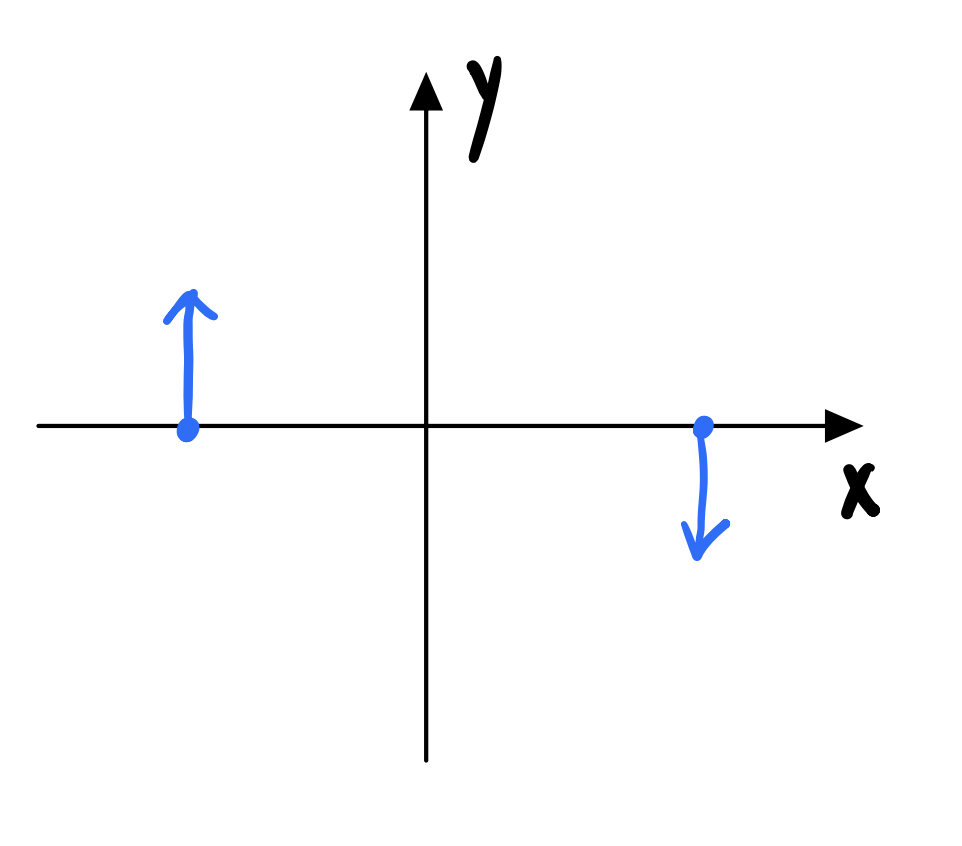
\includegraphics[scale=0.4]{Lectures/Images/lec3-twospinors.png}
\end{center}

We consider a two-point function involving two fermionic fields in the vacuum:
\begin{equation}
    G(x) = \bra{0}D(\pi)\hat{\psi}(\v{x})\hat{\psi}(-\v{x})\ket{0}
\end{equation}
Let us introduce $\hat{U}(\Lambda)\hat{U}(\Lambda)^{-1}$ for $\hat{U}(\Lambda) = \hat{R}$ a rotation by $\pi$. We use the Lorentz invariance of the vaccum, i.e. $\hat{U}(\Lambda)\ket{0} = \ket{0}$.
\begin{equation}
    \begin{split}
        G(x) &= \bra{0}\hat{U}(\Lambda)\hat{U}(\Lambda)^{-1}D(\pi)\hat{\psi}(\v{x})\hat{U}(\Lambda)\hat{U}(\Lambda)^{-1}\hat{\psi}(-\v{x})\hat{U}(\Lambda)\hat{U}(\Lambda)^{-1}\ket{0} 
        \\ &= \bra{0}\hat{U}(\Lambda)^{-1}D(\pi)\hat{\psi}(\v{x})\hat{U}(\Lambda)\hat{U}(\Lambda)^{-1}\hat{\psi}(-\v{x})\hat{U}(\Lambda)\ket{0}
        \\ &= \bra{0}D(\pi)D(\pi)\hat{\psi}(-\v{x})D(\pi)\hat{\psi}(\v{x})\ket{0}
        \\ &= \bra{0}D(2\pi)\hat{\psi}(-\v{x})D(\pi)\hat{\psi}(\v{x})\ket{0}
        \\ &= -\bra{0}\hat{\psi}(-\v{x})D(\pi)\hat{\psi}(\v{x})\ket{0}
    \end{split}
\end{equation}
where in the third equality we note that $\hat{U}(\Lambda)^{-1}\hat{\psi}(\v{x})\hat{U}(\Lambda) = D(\pi)\hat{\psi}(-\v{x})$ and in the final equality we use that $D(2\pi) = -1$ for fermions (note that $D(\pi)$ is just a matrix acting on the indices of $\hat{\psi}$ and so we can move it around freely in the expression). This establishes that the $\psi$ operators have fermionic statistics.

One thing we swept under the rug is the possibility that $G(x) = 0$. This comes from the CPT theorem; invariance under charge/parity/time-reversal symmetry follows that $G(x) > 0$. \qed

Rio note: Asked whether it matters that we only showed it for $\pm \v{x}$ - answer was that it suffices to show it for one correlator. I think maybe you could argue this (from spatial translation/rotation invariance) that all possible coordinate pairs would reduce to the $\pm \v{x}$ case?

Also, note that there are different available proofs of spin-statistics, and each offer a different perspective; see Schwartz for more details and insight.

\subsection{Review of quantizing the free scalar}
We follow Srednicki 37-39 for this discussion.

We recall the Dirac Lagrangian we had constructed:
\begin{equation}
    \mathcal{L} = i\bar{\Psi}\slashed{\p}\Psi - m \bar{\Psi}\Psi
\end{equation}
where $\Psi = \m{\psi_L \\ \psi_R}$ and $\slashed{\p} = \p_\mu \gamma^\mu$ with $\gamma$ matrices:
\begin{equation}
    \gamma^\mu = \m{0 & \sigma^\mu \\ \bar{\sigma}^\mu & 0}
\end{equation}
so:
\begin{equation}
    \slashed{\p} = \m{0 & 0 & \p_0 + \p_3 & \p_1 - i\p_2 \\ 0 & 0 & \p_1 + i\p_2 & \p_0 - \p_3 \\ \ldots & \ldots & 0 & 0 \\ \ldots & \ldots & 0 & 0}.
\end{equation}
We want to quantize this Lagrangian, but let us first review how we quantized the free scalar. For the free scalar that we had the action:
\begin{equation}
    S = -\frac{1}{2}\int (\p\phi)^2 + m^2\phi^2
\end{equation}
the conjugate momenta:
\begin{equation}
    \pi(x) = \frac{\delta S}{\delta \dot{\phi}} = \dot{\phi}
\end{equation}
which obeyed the canonical Poisson bracket relation:
\begin{equation}
    \set{\phi(\v{x}), \pi(\v{y})}_{\text{PB}} = \delta^3(\v{x} - \v{y})
\end{equation}
which we promoted to a commutator relation of operators via canonical quantization:
\begin{equation}
    [\hat{\phi}(\v{x}), \hat{\Pi}(\v{y})] = i\delta^3(\v{x} - \v{y}).
\end{equation}
We had the Hamiltonian, which we quantized and diagonalized:
\begin{equation}
    \begin{split}
        H &= \int \Pi \dot{\phi} - \mathcal{L} 
        \\ &= \int d^3x \frac{1}{2}\Pi^2 + \frac{1}{2}(\nabla \phi)^2 + \frac{1}{2}m^2\phi^2 = \int \frac{d^3k}{(2\pi)^3}\frac{1}{2}\abs{\Pi_\v{k}}^2 + \frac{1}{2}(\v{k}^2 + m^2)\abs{\phi_\v{k}}^2 
        \\ &= \int \frac{d^3k}{(2\pi)^32\e_\v{k}}\e_{\v{k}}a^\dag_{\v{k}}a_{\v{k}}
    \end{split}
\end{equation}
with:
\begin{equation}
    \begin{split}
        a_\v{k} = \e_{\v{k}}\phi_{\v{k}} + i\Pi_{\v{k}}
        \\ a_\v{k}^\dag = \e_{\v{k}}\phi_{-\v{k}} - i\Pi_{-\v{k}}
    \end{split}
\end{equation}
and so:
\begin{equation}
    \phi_{\v{k}} = \frac{1}{2\e_{\v{k}}}(a_{\v{k}} + a_{\v{k}}^\dag)
\end{equation}
so we found the full time evolution of the fields:
\begin{equation}
    \phi(t, \v{x}) = \int \frac{d^3k}{(2\pi)^32\e_{\v{k}}}(a_\v{k}e^{i\v{k} \cdot \v{x}} + a^\dag_{\v{k}}e^{-i\v{k} \cdot \v{x}})
\end{equation}
with $k^0 = \e_{\v{k}} = \sqrt{\v{k}^2 + m^2}$. The Hilbert space of our scalar QFT was Fock space, with:
\begin{equation}
    a_\v{k}\ket{0} = 0 \quad \forall \v{k}
\end{equation}
\begin{equation}
    a^\dag_{\v{k}}\ket{0} = \ket{\v{k}}, a^\dag_{\v{k}_1}a^\dag_{\v{k}_2} = \ket{\v{k}_1, \v{k}_2}, \ldots
\end{equation}

\subsection{Quantizing the Dirac Lagrangian}
With that review under our belt, we want to quantize:
\begin{equation}
    \mathcal{L} = i\bar{\Psi}\gamma^\mu p_\mu \Psi - m\bar{\Psi}\Psi
\end{equation}
so we have the canonical momenta:
\begin{equation}
    \Pi = \frac{\delta S}{\delta \dot{\Psi}} = i\bar{\Psi}\gamma^0 = i\Psi^\dag \gamma^0 \gamma^0 = i\Psi^\dag \implies \Pi_a = i\Psi_a^*
\end{equation}
Thus canonical quantization promotes:
\begin{equation}
    \set{\Psi_a(\v{x}), \Pi_b(\v{y})}_{\text{PB}} = \delta^3(\v{x} - \v{y})\delta_{ab}
\end{equation}
to the commutator:
\begin{equation}
    [\hat{\Psi}_a(\v{x}), \hat{\Pi}_b(\v{y})] = i\delta^3(\v{x} - \v{y})\delta_{ab}.
\end{equation}
The Hamiltonian reads:
\begin{equation}
    H = \Pi\dot{\Psi} - \mathcal{L} = -i\bar{\Psi}\gamma^i\p_i \Psi + m\bar{\Psi}\Psi
\end{equation}

\subsection{General Solution for Dirac Equation}
Let's try to find the most general solution $\Psi(t, \v{x})$ of the Dirac equation:
\begin{equation}
    (i\slashed{\p} - m)\Psi = 0.
\end{equation}
Because $\Psi(x)$ satisfies the Klein-Gordon equation (which follows from the Dirac equation):
\begin{equation}
    (\square + m^2)\Psi = 0
\end{equation}
a general solution will take the form:
\begin{equation}
    \Psi(t, \v{x}) = u(\v{p})e^{ipx} + v(\v{p})e^{-ipx}
\end{equation}
where $u, v$ are 4-component spinors:
\begin{equation}
    u(\v{p}) = \m{u_1(\v{p}) \\ u_2(\v{p}) \\ u_3(\v{p}) \\ u_4(\v{p})}
\end{equation}
and we have the on-shell condition for $p = (p^0, \v{p})$:
\begin{equation}
    p^0 = \e_\v{p} = \sqrt{\v{p}^2 + m^2}.
\end{equation}
But, the solution also has to solve the Dirac equation, which gives us the further condition on the spinors:
\begin{equation}
    0 = (i\slashed{\p} - m)\Psi = (-\slashed{p} - m)u(\v{p})e^{ipx} + (\slashed{p} - m)v(\v{p})e^{-ipx} \implies \begin{cases}
        (\slashed{p} + m)u(\v{p}) = 0
        \\ (\slashed{p} - m)v(\v{p}) = 0
    \end{cases}
\end{equation}
The trick will be to solve these equations in a preferred frame - namely the rest frame, where $ p^\mu_{\text{rest}} = (m, \v{0})$ -  and then boost back to an arbitrary frame $p^\mu = \Lambda^{\mu}_{\sp\nu}p^\nu_{\text{rest}}$:
\begin{equation}
    u(\v{p}) = D(\Lambda)u(\v{0})
\end{equation}
This works because the Dirac equation is Lorentz invariant, but let's check:
\begin{equation}
    \begin{split}
        0 \stackrel{?}{=} (\slashed{p} + m)D(\Lambda)u(\v{0}) &= D(\Lambda)D(\Lambda)^{-1}(\slashed{p} + m)D(\Lambda)u(\v{0}) 
        \\ &= D(\Lambda)(p_\mu D(\Lambda)^{-1}\Gamma^\mu D(\Lambda) - m)u(\v{0})
        \\ &= D(\Lambda)(p_\mu \Lambda^{\mu}_{\sp\nu}\gamma^\nu - m)u(\v{0})
        \\ &= D(\Lambda)(\slashed{p}_{\text{rest}} - m)u(\v{0})
        \\ &= 0.
    \end{split}
\end{equation}
So indeed this strategy works!

In the rest frame we have $p^0_{\text{rest}} = m$ and $p_{0, \text{rest}} = -m$ and so:
\begin{equation}
    \slashed{p}_{\text{rest}} = p_0\gamma^0 = -m\m{0 & \II \\ \II & 0}
\end{equation}
Thus our equation for $u$ is:
\begin{equation}
    m\m{\II & -\II \\ -\II & \II}\m{u_1 \\ u_2 \\ u_3 \\ u_4} = 0
\end{equation}
This implies that $u_1 -u_3 = 0$ and $u_2 -u_4 = 0$. One possible basis for the rest frame solution is therefore:
\begin{equation}
    u_+(\v{0}) = \m{1 \\ 0 \\ 1 \\ 0}, \quad u_-(\v{0}) = \m{0 \\ 1 \\ 0 \\ 1}.
\end{equation}
This basis is convenient because these solutions have a well-defined spin in the $\zhat$-direction (namely $\pm \frac{1}{2}$). Let us do the same for $v$:
\begin{equation}
    m\m{\II & \II \\ \II & \II}\m{v_1 \\ v_2 \\ v_3 \\ v_4} = 0
\end{equation}
This implies that $v_1 + v_3 = 0$ and $v_2 + v_4 = 0$. We then have a basis of solutions:
\begin{equation}
    v_+(\v{0}) = \m{0 \\ 1 \\ 0 \\ -1}, \quad v_-(\v{0}) = \m{-1 \\ 0 \\ 1 \\ 0}
\end{equation}
Now, we boost to get the general solution. What is the Lorentz transformation that takes $p^\mu_{\text{rest}} = (m, \v{0})$ into $p^\mu = (\sqrt{m^2 + \v{p}^2}, \v{p})$? It is clear that we must boost in the $\hat{\v{p}} = \frac{\v{p}}{\abs{\v{p}}}$ direction, so we want the boost $e^{i\eta \hat{\v{p}} \cdot \v{k}}$ by an amount (rapidity) $\eta = \sinh(\frac{\abs{\v{p}}}{m})$. What is then $D(\v{k})$ (representation of boosts on spinors)? This we can construct by recalling that $\v{k} = \frac{\v{J}_+ - \v{J}_-}{i}$ so then:
\begin{equation}
    K_i = \m{\frac{i}{2}\sigma_i & 0 \\ 0 & -\frac{i}{2}\sigma_i}.
\end{equation}
So, in summary:
\begin{equation}
    u(\v{p}) = D(\Lambda)u(\v{0}) = e^{i\eta \hat{p}^iK_i}
\end{equation}
with the $\eta, K_i$ as described the above. There are solutions for $u_\pm, v_\pm$. At the end of the day, a general solution to the Dirac equation takes the form of a most general linear combination of these solutions:
\begin{equation}
    \Psi(t, \v{x}) = \sum_{s = \pm} \int \frac{d^3p}{(2\pi)^32\e_{\v{p}}}[b_s(\v{p})u_s(\v{p})e^{ipx} + d_s^\dag(\v{p})v_s(\v{p})e^{-ipx}]
\end{equation}
Classically, $b, d^\dag$ are coefficients, but after we finish quantizing the theory on Thursday we will see that they play similar roles to the creation/annihilation operators as in the scalar case, and they will create/annihilate spin-1/2 particles. Moreover, we will see that they have to come with a particle-pair; the Dirac equation solutions predict the existence of antiparticles! Historically, this was how the positron (the antiparticle of the electron) was predicted.
\section{The Free Dirac QFT}
\subsection{Reviewing the General Solution}
We found that the general solution to the Dirac equation took the form:
\begin{equation}\label{eq:psix}
    \psi(x) = \sum_{s=\pm}\int \frac{d^3p}{(2\pi)^32\e_\v{p}}\left[b_s(\v{p})u_s(\v{p})e^{ipx} + d^\dag(\v{p})v_s(\v{p})e^{-ipx}\right]
\end{equation}
With:
\begin{equation}
    u_+(\v{0}) = \sqrt{m}\m{1\\0\\1\\0}, \quad u_-(\v{0})=\sqrt{m}\m{0\\1\\0\\1}, \quad v_+(\v{0}) = \sqrt{m}\m{0\\1\\0\\-1}, \quad v_-(\v{0}) = \sqrt{m}\m{-1\\0\\1\\0}
\end{equation}
the spinors in the rest frame, and:
\begin{equation}
    u_s(\v{p}) = \exp(i\sinh^{-1}(\frac{\abs{\v{p}}}{m})\hat{\v{p}}\cdot\v{k})u_s(\v{0})
\end{equation}
(same for the $v_s$) which are the spinors in an arbitrary frame (boosted from the rest frame via $D(\Lambda) = \exp(i\sinh^{-1}(\frac{\abs{\v{p}}}{m})\hat{\v{p}}\cdot\v{k})$). The generators are:
\begin{equation}
    K^i = \m{i\sigma_{i}/2 & 0 \\ 0 & -i\sigma_i/2}, \quad J^i = \m{\sigma_i/2 & 0 \\ 0 & \sigma_i/2}
\end{equation}

\subsection{Spinor relations}
We note that we have the boosted spinor:
\begin{equation}
    u_s(\v{p}) = D(\Lambda)u_s(\v{p})
\end{equation}
and also the barred spinor:
\begin{equation}
    \bar{u}_s(\v{p}) = u_s^\dag(\v{p})\gamma^0 = u_s^\dag(\v{0})D(\Lambda)^\dagger \gamma^0 = \bar{u}_s(\v{0})\gamma^0D(\Lambda)^\dagger \gamma^0 = \bar{u}_s(\v{0}) D(\Lambda)^{-1}
\end{equation}
where we note that $\gamma^0 = \m{0 & \II \\ \II & 0}$ and so $\gamma^0 K_i \gamma^0 = -K_i$ so with the $\theta \leftrightarrow \theta$ flip from the dagger operation we indeed get the inverse transformation. Note that we get simple orthogonality relations between the $u, v$s from studying them in the rest frame:
\begin{equation}
    \bar{u}_s(\v{p})u_{s'}(\v{p}) = \bar{u}_s(\v{0})D(\Lambda)^{-1}D(\Lambda)u_{s'}(\v{0}) = \bar{u}_s(\v{0})u_{s'}(\v{0}) = 2m\delta_{ss'}
\end{equation}
\begin{equation}
    \bar{v}_s(\v{p})\bar{v}_{s'}(\v{p}) = \bar{v}_s(\v{0})v_{s'}(\v{0}) = v_{s'}^\dag(\v{0})\gamma^0v_s(\v{0}) = -2m\delta_{ss'}
\end{equation}
Note that for the $v$s we have minus signs inside of the spinor, so explicitly the $\gamma^0$ becomes relevant.
\begin{equation}
    \bar{v}_s(\v{p})u_{s'}(\v{p}) = 0.
\end{equation}
Let's try computing a slightly more complicated object:
\begin{equation}
    \bar{u}_s(\v{p})\gamma^\mu u_{s'}(\v{p}) = \bar{u}_s(\v{0})D(\Lambda)^{-1}\gamma^\mu D(\Lambda)u_{s'}(\v{0}) = \Lambda^{\mu}_{\sp\nu}\bar{u}_s(\v{0})\gamma^\nu u_{s'}(\v{0}) = \Lambda^{\mu}_{\sp\nu}2m\delta^{\nu}_0 \delta_{ss'} = 2p^\mu \delta_{ss'}
\end{equation}
which we could have partly guessed. There is a very similar equation for the $v$s:
\begin{equation}
    \bar{v}_s(\v{p})\gamma^\mu v_{s'}(\v{p}) = 2p^\mu \delta_{ss'}
\end{equation}
Finally:
\begin{equation}
    \bar{u}_s(\v{p})\gamma^0 v_{s'}(-\v{p}) = u_s^\dag(\v{p})v_{s'}(-\v{p}) = u_s^\dag (\v{0})D(\Lambda)^\dagger D(\Lambda_{-\v{p}})v_{s'}(\v{0}) = u_s^\dag (\v{0})\exp(i\eta\hat{\v{p}} \cdot \v{K})\exp(-i\eta\hat{\v{p}} \cdot \v{K})v_{s'}(\v{0}) = u_s^\dag (\v{0})v_{s'}(\v{0})= 0
\end{equation}

\subsection{Dirac reation and Annihilation Operators}
We will promote $\psi$s to fermionic anticommuting operators. This is fine and dandy, but to extract what the behaviour of $b/d^\dag$ are we will have to use the above spinor technology.

First, let's fourier transform Eq. \eqref{eq:psix}:
\begin{equation}
    \int d^3x e^{-i\v{p}\cdot\v{x}}\psi(x) = \sum_{s=\pm}\frac{1}{2\e_{\v{p}}}[b_s(\v{p})u_s(\v{p}) + d^\dag_s(-\v{p})v_s(-\v{p})]
\end{equation}
Now, we act on the above with $\bar{u}_s(\v{p})\gamma^0$ and use our spinor relations we derived in the previous section:
\begin{equation}
    \begin{split}
        \int d^3xe^{-i\v{p}\cdot\v{x}}\bar{u}_s(\v{p})\gamma^0\psi(x) &= \sum_{s=\pm}\frac{1}{2\e_{\v{p}}}(b_s(\v{p})\bar{u}_s(\v{p})\gamma^0u_{s'}(\v{p}) + d^\dag_s(-\v{p})\bar{u}_s(\v{p})\gamma^0v_s(-\v{p}))
        \\ &= \sum_{s=\pm}\frac{1}{2\e_{\v{p}}}(b_s(\v{p})2p^0\delta_{ss'} + 0)
        \\ &= b_s(\v{p})
    \end{split}
\end{equation}
The analogous barred relation is:
\begin{equation}
    \int d^3x e^{i\v{p}\cdot\v{x}}\bar{\psi}(x)\gamma^0u_s(\v{p}) = b_s^\dag(\v{p}).
\end{equation}

Via canonical quantization, we promote the $\psi$s to operators with the equal time commutation relations:
\begin{equation}
    \set{\psi_a(\v{x}), \psi^\dag_b(\v{0})} = \delta_{ab}\delta^3(\v{x})
\end{equation}
\begin{equation}
    \set{\psi(\v{x}), \psi(\v{0})} = 0
\end{equation}
From this we find that:
\begin{equation}
    \set{b, b} = \set{b^\dag, b^\dag} = 0
\end{equation}
as out expressions for $b, b^\dag$ only involve $\psi, \psi^\dag$s respectively. The only nontrivial relation is the anticommutator between $b$ and $b^\dag$:
\begin{equation}
    \begin{split}
        \set{b_s(\v{p}), b_{s'}^\dag(\v{p}')} &= \int d^3xd^3x' e^{-i(\v{p}\cdot\v{x} - \v{p}'\cdot\v{x}')}\set{\bar{u}_s(\v{p})\gamma^0 \psi(\v{x}), \bar{\psi}(\v{x}')\gamma^0u_s(\v{p})}
        \\ &= \int d^3xd^3x' e^{-i(\v{p}\cdot\v{x} - \v{p}'\cdot\v{x}')} (\bar{u}_s(\v{p})\gamma^0)^a\set{\psi_a(\v{x}), \psi^\dag_b(\v{0})}(\gamma^0\gamma^0u_s(\v{p}))_b 
        \\ &= \int d^3xd^3x' e^{-i(\v{p}\cdot\v{x} - \v{p}'\cdot\v{x}')} (\bar{u}_s(\v{p})\gamma^0)^a\delta_{ab}\delta^3(\v{x}-\v{x}')(\gamma^0\gamma^0u_s(\v{p}))_b 
        \\ &= \int d^3xd^3x' e^{-i(\v{p}\cdot\v{x} - \v{p}'\cdot\v{x}')}\delta^3(\v{x}-\v{x}') \bar{u}_s(\v{p})\gamma^0u_{s'}(\v{p}')
        \\ &= \int d^3x e^{-i(\v{p}-\v{p}')\cdot\v{x}} \bar{u}_s(\v{p})\gamma^0u_{s'}(\v{p}')
        \\ &= \int d^3x e^{-i(\v{p}-\v{p}')\cdot\v{x}}  \delta_{ss'}2p^0
        \\ &= (2\pi)^3\delta^3(\v{p}-\v{p}')\delta_{ss'}2\e_{\v{p}}
    \end{split}
\end{equation}
Now we can do the same with the $d$s. Act on Eq. \eqref{eq:psix} with $\bar{v}_s(-\v{p})\gamma^0$. We then obtain:
\begin{equation}
    d_s^\dag(-\v{p}) = \int d^3x e^{-i\v{p}\cdot\v{x}}v_s(-\v{p})\gamma^0\psi(x)
\end{equation}
and flipping $\v{p} \to -\v{p}$:
\begin{equation}
    d_s^\dag(\v{p}) = \int d^3x e^{i\v{p}\cdot\v{x}}v_s(\v{p})\gamma^0\psi(x)
\end{equation}
Taking the dagger of this relation:
\begin{equation}
    d_s(\v{p}) = \int d^3x e^{-i\v{p}\cdot\v{x}}\bar{\psi}(x)\gamma^0 v_s(\v{p})
\end{equation}
So then:
\begin{equation}
    \set{d, d} = \set{d^\dag, d^\dag} = 0
\end{equation}
and again the only nontrivial relation is between $d, d^\dag$:
\begin{equation}
    \begin{split}
        \set{d_s^\dag(\v{p}), d_{s'}(\v{p}')} &= \int_{\v{x}\v{x}'}e^{i(\v{p} \cdot \v{x} - \v{p}'\cdot\v{x}')}\set{\bar{v}_s(\v{p})\gamma^0\psi(\v{x}), \psi^\dag(\v{x}')\gamma^0v_s(\v{p}')}
        \\ &= \int_{\v{x}\v{x}'}e^{i(\v{p} \cdot \v{x} - \v{p}'\cdot\v{x}')} \delta^3(\v{x}-\v{x}')\bar{v}_s(\v{p})\gamma^0v_{s'}(\v{p}')
        \\ &= \int d^3x e^{i(\v{p} - \v{p}')\cdot\v{x}} 2p^0\delta_{ss'}
        \\ &= (2\pi)^3\delta^3(\v{p} - \v{p}')2\e_{\v{p}}\delta_{ss'}
    \end{split}
\end{equation}
We are almost done. The last thing to check is that the $b, d$ sets of creation/annihilation operators are independent, i.e. that they anticommute. It is clear that:
\begin{equation}
    \set{d^\dag, b} = \set{d, b^\dag} = 0
\end{equation}
and the only potentially nontrivial one we should work through is between $b, d$:
\begin{equation}
    \begin{split}
        \set{b_s(\v{p}), d_{s'}(\v{p}')} &= \int_{\v{x}\v{x}'}e^{-i(\v{p}\cdot\v{x} - \v{p}'\cdot\v{x}')}\set{\bar{u}_s(\v{p})\gamma^0\psi(x), \bar{\psi}(x)\gamma^0v_{s'}(\v{p}')}
        \\ &= \int_{\v{x}\v{x}'}e^{-i(\v{p}\cdot\v{x} - \v{p}'\cdot\v{x}')}\delta^3(\v{x}-\v{x}')\bar{u}_s(\v{p})\gamma^0v_{s'}(\v{p}')
        \\ &= (2\pi)^3\delta^3(\v{p} + \v{p}')\bar{u}_s(\v{p})\gamma^0v_{s'}(-\v{p})
        \\ &= 0
    \end{split}
\end{equation}
so we indeed find that the $b, d$ are independent. The bottom line is we have 4 independent raising and lowering operators $b_\pm, d_\pm$. Notice that $b^\dag \sim \psi^\dag$ while $d^\dag \sim \psi$, so they create particles of opposite ``charge''. What charge?
\begin{equation}
    \mathcal{L} = \bar{\psi}(i\slashed{\p} - m)\psi
\end{equation}
has a $U(1)$ symmetry $\psi \to e^{i\alpha}\psi$. Symmetries imply conservation laws via Noether's theorem - we have the conserved current $\p_\mu j^\mu = 0$. We can identify the Noether charge:
\begin{equation}
    Q = \int d^3x j^0
\end{equation}
which is conserved with $\dot{Q} = 0$. Indeed, we find that:
\begin{equation}
    [Q, \psi^\dag] = i\psi^\dag, \quad [Q, \psi] = -i\psi
\end{equation}
so the two have opposite charge. When we talk about the electron, this Noether charge is just the familiar electric charge, and this is indeed how the Noether charge got its name.

\subsection{Hilbert space of the Dirac Fermion}
We start with the vacuum state $\ket{0}$ annihilated by all annihilation operators:
\begin{equation}
    b_s(\v{p})\ket{0} = d_s(\v{p})\ket{0} = 0 \quad \forall s, \v{p}
\end{equation}
We then have the single particle states:
\begin{equation}
    b_s^\dag(\v{p})\ket{0} = \ket{\v{p}, s, +1}
\end{equation}
which in contrast to the scalar single particle states (which were only labelled by their momentum), are labelled by momentum, spin, and charge. Analogously:
\begin{equation}
    d_s^\dag(\v{p})\ket{0} = \ket{\v{p}, s, -1}
\end{equation}
So for example $\ket{\v{p}, \uparrow, +1} = b^\dag_{\uparrow}(\v{p})\ket{0}$ corresponds to an electron\footnote{Let's take the electron to have positive charge, for now...} with momentum $\v{p}$ and $s_z = +\frac{1}{2}$ and $\ket{\v{p}', \downarrow, -1} = d^\dag_{\downarrow}(\v{p})\ket{0}$ corresponds to a positron with momentum $\v{p}$ and spin $s_z = -\frac{1}{2}$. Multiparticle states are then obtained as:
\begin{equation}
    \begin{split}
        \ket{\ldots, (\v{p}_1, s_1, q_1), \ldots, (\v{p}_2, s_2, q_1), \ldots} &= \ldots b^\dag_{s_1}(\v{p}_1)d^\dag_{s_2}(\v{p}_2)\ldots\ket{0}
        \\ &= \ket{\ldots, n_{\v{p}_1, s_1, q_1} = 1, \ldots, n_{\v{p}_2, s_2, q_2} = 1, \ldots}
    \end{split}
\end{equation}
so we have a bunch of QHO modes labelled by three quantum numbers, but with the distinction to the bosonic case that each mode can only have occupation $ n=0/1$. This is because of the Pauli exclusion principle:
\begin{equation}
    b_{s}^\dag(\v{p})b_s^\dag(\v{p}) = \frac{1}{2}\set{b_{s}^\dag(\v{p}), b_{s}^\dag(\v{p})} = 0
\end{equation}

What is the energy of these particles? We should be able to get this from looking at the commutator of the $b$s with the Hamiltonian:
\begin{equation}
    \begin{split}
        [H, b_s(\v{p})] &= -[b_s(\v{p}), H] 
        \\ &= -\int_{\v{x},\v{x}'}e^{-ipx}[\bar{u}_s(\v{p})\gamma^0\psi(x), \bar{\psi}(x')(-i\gamma^i\p_i + m)\psi(x')]
        \\ &= -\int_{\v{x},\v{x}'}e^{-ipx}\bar{u}_s(\v{p})\gamma^0\set{\psi(x), \psi^\dag(x')}i\gamma^0\gamma^0\p_0 \psi(x')
        \\ &= -\int_{\v{x},\v{x}'}e^{-ipx}\bar{u}_s(\v{p})\gamma^0\delta^3(\v{x}-\v{x}')i\gamma^0\gamma^0\p_0 \psi(x')
        \\ &= -\int d^3x e^{-ipx} \bar{u}_s(\v{p})\gamma^0i\p_0\psi(x)
        \\ &\stackrel{IBP}{=} -p^0\int d^3x e^{-ipx} \bar{u}_s(\v{p})\gamma^0\psi(x)
        \\ &= -\e_\v{p}b_s(\v{p})
    \end{split}
\end{equation}
So $b_s(\v{p})$ lowers the energy by $\e_\v{p} = \sqrt{\v{p}^2 + m^2}$, as expected. Note that the final Hamiltonian has a very simple form in terms of the raising and lowering operators (very similar to the Hamiltonian of a scalar QFT):
\begin{equation}
    H = \sum_s \int \frac{d^3p}{(2\pi)^32\e_{\v{p}}}\e_{\v{p}}(b_s^\dag(\v{p})b_s(\v{p}) + d_s^\dag(\v{p})d_s(\v{p}))
\end{equation}
So this is $H$! What we will then do next week is to study our first fermionic observables in the form of propagators:
\begin{equation}
    \bra{0}\psi_a(\v{x})\bar{\psi}_b(\v{y})\ket{0}
\end{equation}
\begin{equation}
    \bra{0}\mathcal{T}\psi_a(\v{x})\bar{\psi}_b(\v{y})\ket{0}
\end{equation}
We will do a lot of work to get a simple answer, then wonder if there was a simpler way, and in fact we will find that the simple method is using the path integral - the twist there will be that we integrate over a Grassman variable.
\section{The Fermion Propagator}
The relevant section is Srednicki 42.

We want to compute correlation functions fermions, e.g. $\bra{0}\bar{\psi}_a\psi_b\psi_c\bar{\psi}_d\ket{0}$. Through the LSZ formula, they will be related to $e^+/e^-$ scattering. These correlators are also observables in their own right - for example the current (observable in CM experiments) goes as $\avg{j^\mu j^\nu} \sim \avg{\bar{\psi}\gamma^\mu \psi \bar{\psi}\gamma^\nu \psi}$.

\begin{center}
    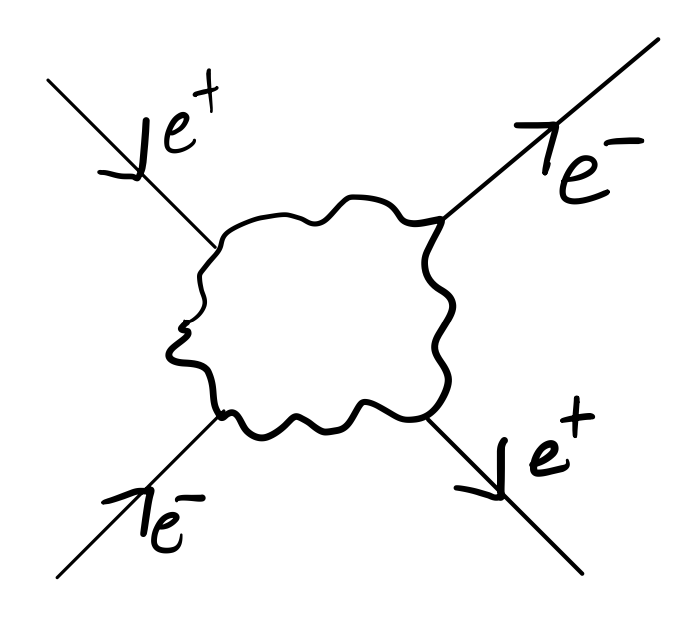
\includegraphics[scale=0.3]{Lectures/Images/lec5-elecpositscattering.png}
\end{center}

Today, we look at the simplest observable, the propagator/2-point function:
\begin{equation}
    G_W(x)_{\alpha\beta} = \bra{0}\psi_\alpha(x)\bar{\psi}_\beta(0)\ket{0}
\end{equation}
\begin{equation}
    G_F(x)_{\alpha\beta} =  \bra{0}\mathcal{T}\psi_\alpha(x)\bar{\psi}_\beta(0)\ket{0}
\end{equation}
Where for fermions:
\begin{equation}
    \mathcal{T}\psi_\alpha(x)\psi_\beta(0) = \begin{cases}
        \psi_\alpha(x)\bar{\psi}_\beta(0) & \text{if $x^0 > 0$}
        \\ -\bar{\psi}_\beta(0)\psi_\alpha(0) & \text{if $x^0 < 0$}
    \end{cases}
\end{equation}

\subsection{Computing the 2-point function}
We compute the 2-point function by plugging in our expression for $\psi(x)$ that we found last week:
\begin{equation}
    \psi(x) = \sum_{s=\pm}\int \frac{d^3p}{(2\pi)^32\e_\v{p}}\left[b_s(\v{p})u_s(\v{p})e^{ipx} + d^\dag(\v{p})v_s(\v{p})e^{-ipx}\right]
\end{equation}
Therein:
\begin{equation}
    \bra{0}\psi_\alpha(x)\bar{\psi}_\beta(0)\ket{0} = \sum_{ss'}\int_{pp'} u_s(\v{p})e^{ipx}\bra{0}b_s(\v{p})b_{s'}^\dag(\v{p}')\ket{0}\bar{u}_{s', \beta}(\v{p}')e^{-ip'\cdot 0}
\end{equation}
where we use that the annihilation operator annihilates the vacuum, making the $d$-pieces of the expression zero. We can, for free, replace $b_s(\v{p})b_{s'}^\dag(\v{p}')$ by an anticommutator since $b_s$ annihilates the vacuum. Then, since $\set{b_s(\v{p}), b_{s'}^\dag(\v{p}')} = (2\pi)^3\delta^3(\v{p} - \v{p}')2\e_{\v{p}}\delta_{ss'}$, this allows us to get rid of the $\v{p}'$ integral and the $s'$ sum, leaving us with:
\begin{equation}
    \bra{0}\psi_\alpha(x)\bar{\psi}_\beta(0)\ket{0} = \int \frac{d^3p}{(2\pi)^32\e_\v{p}}\sum_{s=\pm}u_{s, \alpha}(\v{p})\bar{u}_{s, \beta}(\v{p}) e^{ipx}
\end{equation}
This simplifies via the completeness relation:
\begin{equation}
    \sum_{s=\pm}u_{s, \alpha}(\v{p})\bar{u}_{s, \beta}(\v{p}) = (-\slashed{p} + m)_{\alpha\beta}
\end{equation}
Which can be seen by computing it in the rest frame with $p_\mu^{\text{rest}} = (-m, \v{0})$:
\begin{equation}
    u_+ = \sqrt{m}\m{1\\0\\1\\0}, \quad  u_- = \sqrt{m}\m{0\\1\\0\\1}, \quad \bar{u} = \gamma^0u = \m{0 & \II \\ \II & 0}u
\end{equation}
\begin{equation}
    u_+u_+^\dag = m\m{1\\0\\1\\0}\m{1&0&1&0} = m\m{1 & 0 & 1 & 0 \\ 0 & 0 & 0 & 0 \\ 1 & 0 & 1 & 0 \\ 0 & 0 & 0 & 0}
\end{equation}
\begin{equation}
    u_-u_-^\dag = m\m{0 & 0 & 0 & 0 \\ 0 & 1 & 0 & 1 \\ 0 & 0 & 0 & 0 \\ 0 & 1 & 0 & 1}
\end{equation}
thus:
\begin{equation}
    \sum_{s=\pm}u_s u_s^\dag = m\m{\II & \II \\ \II & \II} = m\II + m\gamma^0 = m\II - p_0^{\text{rest}}\gamma^0
\end{equation} 
Then we can act with our boost generators on the left and right to get the expression in a general frame:
\begin{equation}
    \sum_s u_s(\v{p})\bar{u}_s(\v{p}) = m\II - p_\mu \gamma^\mu
\end{equation}
which gives a simple final expression:
\begin{equation}
    \bra{0}\psi_\alpha(x)\bar{\psi}_\beta(0)\ket{0} = \int \frac{d^3p}{(2\pi)^32\e_\v{p}}(m - \slashed{p})_{\alpha\beta} e^{ipx}
\end{equation}
Since we are interested in the time-ordered correlation function, we should also look at the correlation function with the two field operators swapped:
\begin{equation}
    \bra{0}\bar{\psi}_\beta(0)\psi_\alpha(x)\ket{0} = \sum_{ss'}\int_{pp'}\bar{v}_{s, \beta}(\v{p})\bra{0}d_s(\v{p})d_{s'}(\v{p}')\ket{0}v_{s'\alpha}(\v{p})e^{-ip'x}
\end{equation}
We again replace $d_s(\v{p})d_{s'}(\v{p}')$ by the anticommutator, which kills the $s'$ and $p'$ sums:
\begin{equation}
    \bra{0}\bar{\psi}_\beta(0)\psi_\alpha(x)\ket{0} = \int \frac{d^3p}{(2\pi)^32\e_\v{p}}\sum_s \bar{v}_{s, \beta}(\v{p})v_{s, \alpha}(\v{p})e^{-ipx} = \int \frac{d^3p}{(2\pi)^32\e_\v{p}}(-\slashed{p}-m)_{\alpha\beta}e^{-ipx}
\end{equation}
where we have used the analogous completeness relation in the last equality. The bottom line is that the time-ordered Green's function looks like:
\begin{equation}
    G_F(x) = \int \frac{d^3p}{(2\pi)^32\e_{\v{p}}}\Theta(x^0)(m-\slashed{p})e^{ipx} + \Theta(-x^0)(\slashed{p} + m)e^{-ipx}
\end{equation}


\subsection{Lorentz-Covariant 2-point function}
but there is a slightly nicer way to write this in a way that makes the expression manifestly Lorentz covariant. We will simplify it via an identity involving the integral:
\begin{equation}
    \int \frac{d^4p}{(2\pi)^4}\frac{e^{ipx}}{p^2 + m^2 - i0^+}f(p^\mu)
\end{equation}
where we note that $px = -p^0x^0 + \v{p}\cdot\v{x}$, where $p^0$ is a free variable that is integrated over. The expression (as in the case of a free scalar) has two poles, at:
\begin{equation}
    p^0 = \pm(\e_\v{p} - i0^+)
\end{equation}

\begin{center}
    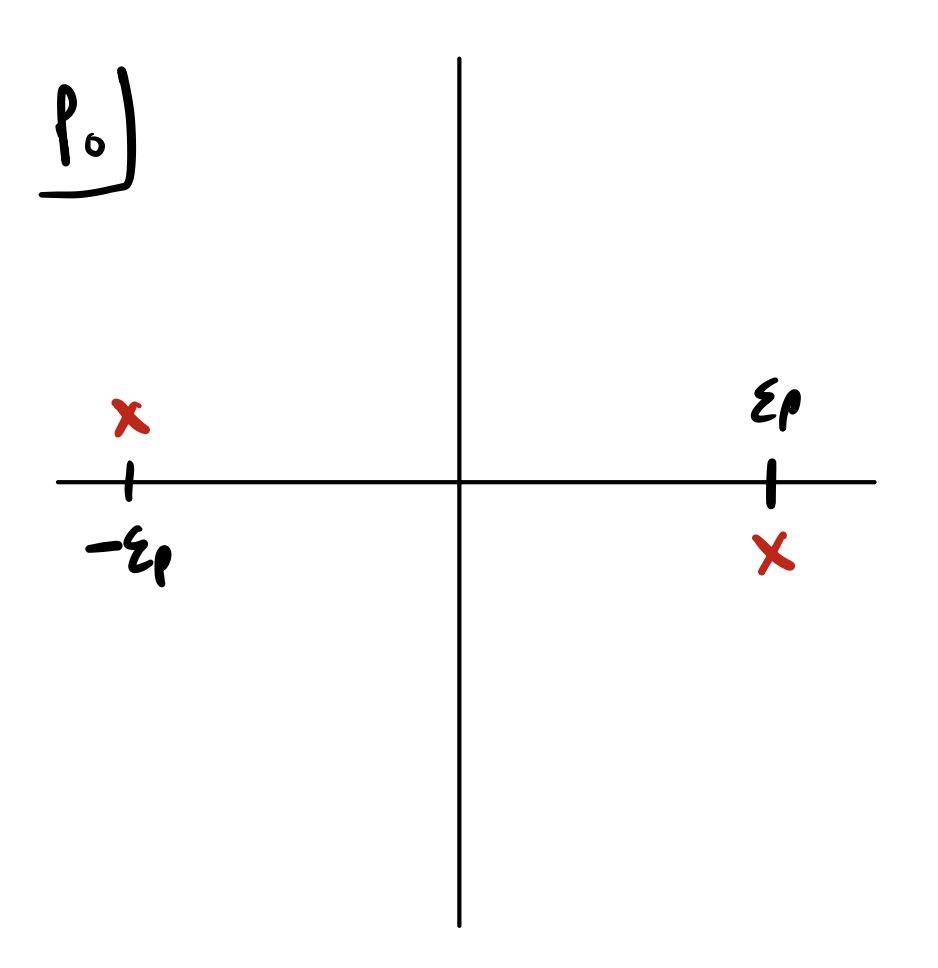
\includegraphics[scale=0.3]{Lectures/Images/lec5-p0poles.png}
\end{center}

This will allow us to carry out the integral over $p^0$, leaving us with a integral over spatial momentum; reversing the process we will obtain an expression for $G_F(x)$. If $x^0 > 0$, we will want to close the contour in the lower half plane, and vise versa if $x^0 < 0$ (in order for the integral to converge):
\begin{equation}
    \begin{split}
        \int \frac{d^4p}{(2\pi)^4}\frac{e^{ipx}}{p^2 + m^2 - i0^+}f(p^\mu) &= -\Theta(x^0)\int \frac{d^3p}{(2\pi)^4}(-2\pi i)\frac{e^{i(\e_p x^0 + \v{p} \cdot \v{x})}}{2\e_\v{p}}f(\e_\v{p}, \v{p}) - \Theta(-x^0)\int \frac{d^3p}{(2\pi)^4}(2\pi i)\frac{e^{i(-\e_p x^0 + \v{p} \cdot \v{x})}}{-2\e_p}f(-\e_\v{p}, \v{p})
        \\ &= i\int \frac{d^3p}{(2\pi)^32\e_{\v{p}}}\left[\Theta(x^0)e^{ipx}f(\e_\v{p}, \v{p}) + \Theta(-x^0)e^{-ipx}f(-\e_{\v{p}}, -\v{p})\right]
    \end{split}
\end{equation}
Now we have something that looks exactly like what we have for $G_F(x)$, so using this identity:
\begin{equation}
    \boxed{G_F(x) = -i\int \frac{d^4p}{(2\pi)^4}e^{ipx}\frac{m-\slashed{p}}{p^2 + m^2 - i0^+}}
\end{equation}
Fourier transforming, we have:
\begin{equation}
    \boxed{G_F(p) = \int d^4x e^{-ipx}G_F(x) = -i\frac{m-\slashed{p}}{p^2 + m^2 - i0^+}}
\end{equation}
This looks pretty similar to the scalar field propagator, up to the extra factor $m - \slashed{p}$. It's not so surprising that it looks similar, because the fermionic fields also satisfy the Klein-Gordon equation.

Note that:
\begin{equation}
    \begin{split}
        (m + \slashed{p})(m - \slashed{p}) &= m^2 - \slashed{p}^2 
        \\ &= m^2 - p_\mu p_\nu \gamma^\mu \gamma^\nu
        \\ &= m^2 - p_\mu p_\nu \left(\frac{1}{2}\set{\gamma^\mu, \gamma^\nu}\right)
        \\ &= m^2 - p_\mu p_\nu (-\eta^{\mu\nu})
        \\ &= m^2 + p^2
    \end{split}
\end{equation}
Which allows us to write the inverse:
\begin{equation}
    (m + \slashed{p})^{-1} = \frac{m - \slashed{p}}{m^2 + p^2}
\end{equation}
Thus we may also write the Feynman Green's function as:
\begin{equation}
    G_F^\psi(p) = \frac{-i}{m + \slashed{p}}
\end{equation}
This is interesting! Remember for scalars that:
\begin{equation}
    G_F^\phi(p) = \frac{-i}{p^2 + m^2}
\end{equation}
This was the ``inverse of the equation of motion'', and indeed we find the same for $G^\psi_F$:
\begin{equation}
    -(m + \slashed{p})G_F(p) = i \implies \int \frac{d^4p}{(2\pi)^4}e^{ipx}(-\slashed{p} - m)G_F(p) = i\delta^4(x)
\end{equation}
Note that we can write the $\slashed{p}$ as a derivative:
\begin{equation}
    (i\slashed{p} - m)\int \frac{d^4p}{(2\pi)^4}e^{ipx}G_F(p) = i\delta^4(x)
\end{equation}
and thus:
\begin{equation}
    \boxed{(i\slashed{p} - m)G_F(x) = i\delta^4(x)}
\end{equation}
which is the formal notion in which the Green's function is the inverse of the EoM/Dirac equation in this case.

\subsection{Path Integral for Fermions - Desiderata}
We may now ask if there would have been a simpler/more direct way to get to this result - for the scalar field there indeed was, via the path integral formalism. The same will be true for fermions!

Recall for the scalar field that:
\begin{equation}
    \begin{split}
        \avg{\mathcal{T}\phi(x)\phi(0)} &= \int \mathcal{D}\phi \phi(x)\phi(0)\frac{e^{i\int \phi(\p^2 - m^2)\phi}}{\int \mathcal{D}\phi e^{iS}}
        \\ &= \frac{1}{Z}\frac{\delta^2}{i\delta J(x) i\delta J(0)} \left.\int \mathcal{D}\phi e^{i\int \phi(\p^2 - m^2)\phi + J\phi}\right|_{J = 0}
        \\ &= \frac{1}{Z}\frac{\delta^2}{i\delta J(x) i\delta J(0)} \left.\int \mathcal{D}\phi \exp(\frac{i}{2}\int (\phi + D^{-1}J)D(\phi + D^{-1}J) - JD^{-1}J)\right|_{J=0}
        \\ &= \left.frac{\delta^2}{i\delta J(x) i\delta J(0)} e^{-\frac{i}{2}\int JD^{-1}J}\right|_{J=0}
        \\ &= \frac{-i}{-\p^2 + m^2}
    \end{split}
\end{equation}

We now want a similar formalism for fermions; we would like:
\begin{equation}
    \begin{split}
        \bra{0}\mathcal{T}\psi_{\alpha}(x)\bar{\psi}_\beta(0)\ket{0} &= \int \mathcal{D}\psi \psi_{\alpha}(x)\bar{\psi}_{\beta}(0)e^{i\int d^4x \bar{\psi}(i\slashed{p} - m)\psi}/\int \mathcal{D}\psi e^{iS}
        \\ &= \frac{\delta^2}{\delta i \bar{\eta}_{\alpha}(x) \delta i \eta_{\beta}(x)}\left.\int \mathcal{D}\psi e^{i\int \bar{\psi} D \psi + \bar{\psi}\eta + \bar{\eta}\psi}\right|_{\eta=0}/\int \mathcal{D}\psi e^{iS}
        \\ &= \frac{\delta^2}{\delta i \bar{\eta}_{\alpha}(x) \delta i \eta_{\beta}(x)}\left.e^{i\int \bar{\eta}D^{-1}\eta}\right|_{\eta=0}/\int \mathcal{D}\psi e^{iS}
        \\ &= -\frac{i}{i\slashed{p} - m}
    \end{split}
\end{equation}

But for this to work, we require that the variable of integration $\psi$, as well as the source $\eta$, have to anticommute; they are Grassman numbers, where $\psi_1\psi_2 = -\psi_2\psi_1$. The approach that Srednicki takes in Section 44 is that one can define numbers with the desired property and the formalism carries through - i.e. he mostly says that ``it works''. But here, we will try to actually derive it.

\subsection{Reviewing the Bosonic SHO Path Integral Derivation}
Recall the Bosonic SHO; we had the action and Hamiltonian:
\begin{equation}
    S = \int dt \frac{1}{2}m\dot{q}^2 - \frac{1}{2}kq^2 \implies \hat{H} = \frac{\hat{p}^2}{2m} + \frac{1}{2}k\hat{q}^2
\end{equation}
Then we could consider the evolution via $e^{-i\hat{H}t} = \prod_{i=1}^N e^{-i\hat{H}\delta t}$:
\begin{equation}
    \bra{q_f}e^{-i\hat{H}t}\ket{q_i} = \int \prod_{j=1}^N dq_j dp_j \ldots \bra{q_2}e^{-i\hat{H}\delta t}\ket{p_1}\braket{p_1}{q_1}
\end{equation}
then using that:
\begin{equation}
    \bra{q_2}e^{-i\hat{H}\delta t}\ket{p_1} = e^{-i\left(\frac{p_1^2}{2m} + \frac{1}{2}kq_2^2\right)\delta t}\braket{q_2}{p_1}\braket{p_1}{q_1} = e^{-i\left(\frac{p_1^2}{2m} + \frac{1}{2}kq_2^2\right)\delta t}e^{ip_1(q_2 - q_1)}
\end{equation}
So then carrying out the Gaussian integral over $p_1$:
\begin{equation}
    \bra{q_f}e^{-i\hat{H}t}\ket{q_i} = \int \prod_{j=1}^N dq_j dp_j \ldots e^{i\left(\frac{1}{2}m\frac{(q_2 - q_1)^2}{\delta t^2} - \frac{1}{2}kq_2^2\right)\delta t} = \int \prod_{j=1}^N dq_j dp_j \ldots e^{i\left(\frac{1}{2}m\dot{q}^2 - \frac{1}{2}kq_2^2\right)\delta t} 
\end{equation}
then recognizing that what is left in the exponential is just the action, we could write:
\begin{equation}
    \bra{q_f}e^{-i\hat{H}t}\ket{q_i} = \int \mathcal{D}q e^{iS}
\end{equation}

\subsection{Deriving the Fermionic Path Integral}
Now consider:
\begin{equation}
    S = \int dt \psi^\dag (i\p_t - m)\psi \implies \hat{H} = m\hat{\psi}^\dag \hat{\psi}
\end{equation}
where $\hat{\psi}^2 = 0$. There is the ground state $\ket{0}$ annihilated by $\hat{\psi}$, and the state with one particle, $\hat{\psi}^\dag\ket{0} = \ket{1}$. And then - we're done. We can't keep acting on this state with $\hat{\psi}^\dag$, because this would give us zero. There are only two states in the Hilbert space, defined by:
\begin{equation}
    \hat{\psi}\ket{0} = 0
\end{equation}
\begin{equation}
    \hat{\psi}\ket{1} = \hat{\psi}\hat{\psi}^\dag \ket{0} = \set{\hat{\psi}, \hat{\psi}^\dag}\ket{0} = \ket{0}
\end{equation}
What was crucial in the bosonic QHO derivation was the eigenstates of the annihilation/creation operators - the coherent states. Here, we look at our defining relations, and $\hat{\psi}$ annihilates $\ket{0}$ and sends $\ket{1}$ to $\ket{0}$, which makes constructing an eigenstate... impossible, if we consider regular coefficients. But if we allow for coefficients which are Grassman numbers, then we can do this! We can define:
\begin{equation}
    \ket{\eta} = \ket{0} + \ket{1}\eta
\end{equation}
where then:
\begin{equation}
    \hat{\psi}\ket{\eta} = 0 + \ket{0}\eta = \ket{\eta}\eta
\end{equation}
if we let $\eta^2 = 0$. So, with these interesting objects of Grassman numbers, we can build eigenstates of $\hat{\psi}$. Similarly, we define:
\begin{equation}
    \bra{\eta^\dag} = \bra{0} + \eta^\dag\bra{1} \implies \bra{\eta^\dag}\hat{\psi}^\dag = \eta^\dag \bra{\eta^\dag}
\end{equation}
What is the overlap between the fermionic coherent states? We calculate:
\begin{equation}
    \braket{\eta_1}{\eta_2} = (\bra{0} + \eta_1^\dag\bra{1})(\ket{0} + \ket{1}\eta_2) = 1 + \eta_1^\dag \eta_2 = e^{\eta_1^\dag \eta_2}
\end{equation}
Writing this as an exponential seems strange, but it is completely correct. If we taylor expand, all second order terms and higher vanish as Grassman numbers square to zero. But this form does make the analogy with the bosonic case more clear. With this, we can now define the fermionic path integral:
\begin{equation}
    \begin{split}
        \bra{\psi_f}e^{-i\hat{H}t}\ket{\psi_i} &= \int \prod_{j=1}^N d\psi_j d\psi_j^\dag \ldots \bra{\psi_2}e^{-iH\delta t}\ket{\psi_1^\dag}\braket{\psi_1^\dag}{\psi_1}
        \\ &=  \int \prod_{j=1}^N d\psi_j d\psi_j^\dag \ldots e^{-im\psi^\dag \psi_2 \delta t}\braket{\psi_2}{\psi_1^\dag}\braket{\psi_1^\dag}{\psi_2}
        \\ &= \int \prod_{j=1}^N d\psi_j d\psi_j^\dag \ldots e^{-im\psi^\dag_1 \psi_2 \delta t}e^{-\eta_1^\dag(\eta_2 - \eta_1)}
        \\ &= \int \prod_{i=1}^N d\psi_j \ldots e^{i(\psi_1^\dag i(\psi_2 - \psi_1) - m\psi_1^\dag \psi_2)\delta t}
        \\ &\stackrel{N\to\infty}{\to} \int D\psi D\psi^\dag e^{i\int dt \psi^\dag (i\p_t - m)\psi}
    \end{split}
\end{equation}
and in fact we are done; in the scalar case we integrated out the momenta ($p$), here we keep it ($\psi^\dag$). So, we have our expression for a single fermion; on Thursday we will generalize this to the Dirac fermion.
\section{Path Integral for Dirac QFT, Interacting Fermions}
Last lecture, we found a path integral representation for fermionic quantum mechanics (wherein we had to replace the variables being integrated over by Grassman numbers):
\begin{equation}
    Z = \int \mathcal{D}\psi \mathcal{D}\psi^\dag e^{i\int dt \psi^\dag (i\p_t - m)\psi}
\end{equation}

\subsection{Generating Functional + Two-Point Function for Dirac QFT}
For the Dirac QFT, we can consider the generating functional:
\begin{equation}
    Z[\eta, \bar{\eta}] = \int \mathcal{D}\psi \mathcal{D}\psi^\dag e^{i\int d^4x \bar{\psi}(i\slashed{\p} - m)\psi + \bar{\psi}\eta + \bar{\eta}\psi}
\end{equation}
From this, we can obtain the time-ordered two-point function (keeping in mind that these are Grassman numbers, so introducing minus signs accordingly where we would need to move the derivative past a grassman number) via:
\begin{equation}
    \begin{split}
        \bra{0}\mathcal{T}\psi(x)\bar{\psi}(0)\ket{0} &= \frac{1}{Z[0, 0]}\int \mathcal{D}\psi\mathcal{D}\psi^\dag \psi(x)\bar{\psi}(0)e^{iS} 
        \\ &= \frac{1}{Z[0, 0]}\int \mathcal{D}\psi\mathcal{D}\psi^\dag\left(\frac{\delta}{i\delta \bar{\eta}(x)}\right) \left(-\frac{\delta}{i\delta \eta(0)}\right) e^{i\int \bar{\psi}(i\slashed{\p} - m)\psi + \bar{\psi}\eta + \bar{\eta}\psi}
        \\ &= \frac{1}{Z[0, 0]}\left.\frac{\delta^2}{\delta \bar{\eta}(x)\delta \eta(0)}Z[\eta, \bar{\eta}]\right|_{\eta=0}
        \\ &= \left.\frac{\delta^2}{\delta \bar{\eta}(x)\delta \eta(0)}\log Z[\eta, \bar{\eta}]\right|_{\eta=0}
    \end{split}
\end{equation}
We can thus compute fermionic correlation functions via a path integral (note that we compute the connected correlation function above, which coincides with the disconnected correlation function here as the one point functions vanish). We will find that we can exactly perform the integral for $Z[\eta, \bar{\eta}]$ and so this fully solves the theory; all correlation functions can then be obtained as functional derivatives of the generating functional. Let's carry out this integral:
\begin{equation}
    Z{\eta, \bar{\eta}} = \int \mathcal{D}\psi \mathcal{D}\psi^\dag e^{-i\int \frac{d^4p}{(2\pi)^4}\bar{\psi}_p(-\slashed{p} + m)\psi_p - \bar{\psi}_p\eta_p - \bar{\eta}_p\psi_p}
\end{equation}
We complete the square; we want this to look like the Gaussian integral with argument $\bar{\chi}_p(\slashed{p} + m)\chi_p$, which motivates the definition of:
\begin{equation}
    \begin{split}
        \chi_p &= \psi_p - (\slashed{p} + m)^{-1}\eta_p
        \\ \bar{\chi}_p &= \bar{\psi}_p - \eta^\dag_p(\slashed{p}^\dag + m)^{-1}\gamma^0
    \end{split}
\end{equation}
where we note that:
\begin{equation}
    \gamma^0(\slashed{p})^\dag\gamma^0 = \slashed{p}
\end{equation}
which follows from:
\begin{equation}
    \gamma^0(\gamma^\mu)^\dag\gamma^0 = \gamma^\mu
\end{equation}
Of course with this substitution we end up with a term quadratic in the $\eta$s:
\begin{equation}
    \bar{\psi}_p(-\slashed{p} + m)\psi_p - \bar{\psi}_p\eta_p - \bar{\eta}_p\psi_p = \bar{\chi}_p(\slashed{p} + m)\chi_p - \bar{\eta}_p(\slashed{p} + m)^{-1}\eta_p
\end{equation}
so our generating functional becomes:
\begin{equation}
    Z[\eta, \bar{\eta}] = \left(\int \mathcal{D}\chi \mathcal{D}\chi^\dag e^{-i\int \frac{d^4p}{(2\pi)^4}\bar{\chi}_p(\slashed{p} + m)\chi_p}\right)e^{i\int \frac{d^4p}{(2\pi)^4}\bar{\eta}_p(\slashed{p} + m)^{-1}\eta_p} = Z[0, 0]e^{i\int \frac{d^4p}{(2\pi)^4}\bar{\eta}_p(\slashed{p} + m)^{-1}\eta_p} 
\end{equation}
Thus:
\begin{equation}
    \log Z[\eta, \bar{\eta}] = \log Z[0, 0] + i\int \frac{d^4p}{(2\pi)^4}\bar{\eta}_p(\slashed{p} + m)^{-1}\eta_p
\end{equation}
Writing this in position space (and leaving off the constant $\log Z[0, 0]$):
\begin{equation}
    \log Z[\eta, \bar{\eta}] = \int d^4x d^4x'\frac{d^4p}{(2\pi)^4}\bar{\eta}(x)\frac{e^{ip(x - x')}}{\slashed{p} + m}\eta(x') = -\int d^4x d^4x' \bar{\eta}(x)G_F(x-x')\eta(x')
\end{equation}
Thus taking two derivatives, we find (as we did found in the canonical quantization calculation we did last class):
\begin{equation}
    \bra{0}\mathcal{T}\psi(x)\bar{\psi}(0)\ket{0} = \left.\frac{\delta^2}{\delta \bar{\eta}(x)\delta \eta(0)}\log Z[\eta, \bar{\eta}]\right|_{\eta=0} = G_F(x)
\end{equation}

\subsection{Wick's theorem for fermions}
So we have rederived the expression for the two-point function, but we have done a lot more; we now have a simple way to compute arbitrary correlation functions. We have shown the generating functional is quadratic in $\eta$, implying a version of Wick's theorem for fermions. For example, looking at the connected four-point function (which vanishes):
\begin{equation}
    \begin{split}
        0 &= \left.\frac{\delta^4}{\delta\eta_1\delta\eta_2\delta\eta_3\delta\eta_4}\log Z\right|_{\eta=0} 
        \\ &= \p_{\eta_1}\p_{\eta_2}\p_{\eta_3}\left(\frac{\p_{\eta_4} Z}{Z}\right) 
        \\ &= \p_{\eta_1}\p_{\eta_2}\left(\frac{\p_{\eta_3}\p_{\eta_4}Z}{Z} - \frac{\p_{\eta_3}Z\p_{\eta_4}Z}{Z}\right)
        \\ &= \p_{\eta_1}\left(\frac{\p_{\eta_2}\p_{\eta_3}\p_{\eta_4}Z}{Z} - \frac{\p_{\eta_3}\p_{\eta_4}Z\p_{\eta_2}Z}{Z^2} - \frac{\p_{\eta_2}\p_{\eta_3}Z\p_{\eta_4}Z}{Z^2} \textcolor{red}{+} \frac{\p_{\eta_3}Z\p_{\eta_2}\p_{\eta_4}Z}{Z^2}\right)
        \\ &= \frac{\p_{\eta_1}\p_{\eta_2}\p_{\eta_3}\p_{\eta_4}Z}{Z} - \frac{\p_{\eta_3}\p_{\eta_4}Z\p_{\eta_1}\p_{\eta_2}Z}{Z^2} - \frac{\p_{\eta_2}\p_{\eta_3}Z\p_{\eta_1}\p_{\eta_4}Z}{Z^2} + \frac{\p_{\eta_1}\p_{\eta_3}Z\p_{\eta_2}\p_{\eta_3}Z}{Z^2}
    \end{split}
\end{equation}
where in the fourth and fifth equality we use that the one-point function vanishes and hence we can discard any terms of the form of $\left. \p_{\eta}Z \right|_{\eta=0} = 0$. Note the sign of the last term in the fourth equality, which arises from moving the $\p_{\eta_2}$ derivative past the $\p_{\eta_3}Z$, which results in an extra negative sign as these are anticommuting numbers - this is the only distinction from the analogous calculation we did for the scalar QFT. Thus, writing the four-point function in terms of two point functions:
\begin{equation}
    \avg{\psi_1\psi_2\psi_3\psi_4} = \avg{\psi_1\psi_2}\avg{\psi_3\psi_4} + \avg{\psi_2\psi_3}\avg{\psi_1\psi_4} - \avg{\psi_1\psi_3}\avg{\psi_2\psi_4}
\end{equation}
which we can see is a sum over all pairings, except every time we have to move fermionic variables across each other to pair them we introduce a minus sign. The above result hinges on the fact that:
\begin{equation}
    \left.\frac{\delta^4}{\delta\eta_1\delta\eta_2\delta\eta_3\delta\eta_4}\log Z\right|_{\eta=0}  = 0
\end{equation} 
which is true for free Dirac theories (for which the generating functional is quadratic in the sources).

Of course, its worth noting that throughout we have suppressed the indices above, but each of the $\psi$s are spinors, so these are really all matrix equations.

\subsection{Interacting Fermions - Yukawa Theory}
There are many theories of interacting fermions in nature - the main focus of our study will be QED, but we will look at a simpler theory first; namely coupling a scalar and a Dirac fermion.

To review, we have the Lagrangian for the free scalar:
\begin{equation}
    \mathcal{L}_\phi = -\frac{1}{2}(\p\phi)^2 - \frac{1}{2}M^2\phi^2
\end{equation}
and the Lagrangian for the free Dirac fermion:
\begin{equation}
    \mathcal{L}_\psi = \bar{\psi}(i\slashed{p} - m)\psi
\end{equation}
We can of course have these theories as independent/non-interacting, but let's make them talk to each other! How can we couple the two? The simplest way we may couple the two is:
\begin{equation}
    \mathcal{L}_{\text{Yukawa}} = \lambda \phi \bar{\psi}\psi
\end{equation}
which is indeed a Lorentz-invariant scalar, as we require. You will explore this theory in PS3. When building a theory, it is good to start off with the simplest interactions possible (i.e. contain the least number of derivatives possible), as these are the most relevant interactions (as we can ascertain via dimensional analysis).

This interaction will lead to a correlation, which we can compute perturbatively in the usual way using the path integral formalism; to first order:
\begin{equation}
    \begin{split}
        \bra{0}\phi(x_1)\psi(x_2)\bar{\psi}(x_3)\ket{0} &\cong \avg{iS_{\text{int}}\phi(x_1)\phi(x_2)\bar{\psi}(x_3)}_{\text{free}}
        \\ &= i\lambda \int d^4x \avg{\phi(x)\bar{\psi}(x)\psi(x) \phi(x_1)\psi(x_2)\bar{\psi}(x_3)}_{\text{free}}
        \\ &= i\lambda \int d^4x G_F^\phi(x - x_1)\avg{\psi(x_2)\bar{\psi}(x)\psi(x)\bar{\psi}(x_3)}
        \\ &= i\lambda \int d^4x G_\phi^F(x - x_1)G_\psi^F(x_2 - x)G^F_\psi(x - x_3)
    \end{split}
\end{equation}
We have contracted the two scalar fields together (the only nonvanishing contraction in the free theory), as well as $\psi(x_2)$ with $\bar{\psi}(x)$ and $\psi(x)$ with $\bar{\psi}(x_3)$ such that the Feynman diagram is connected (and hence nonvanishing). In position space, we can imagine this Feynman diagram as:

\begin{center}
    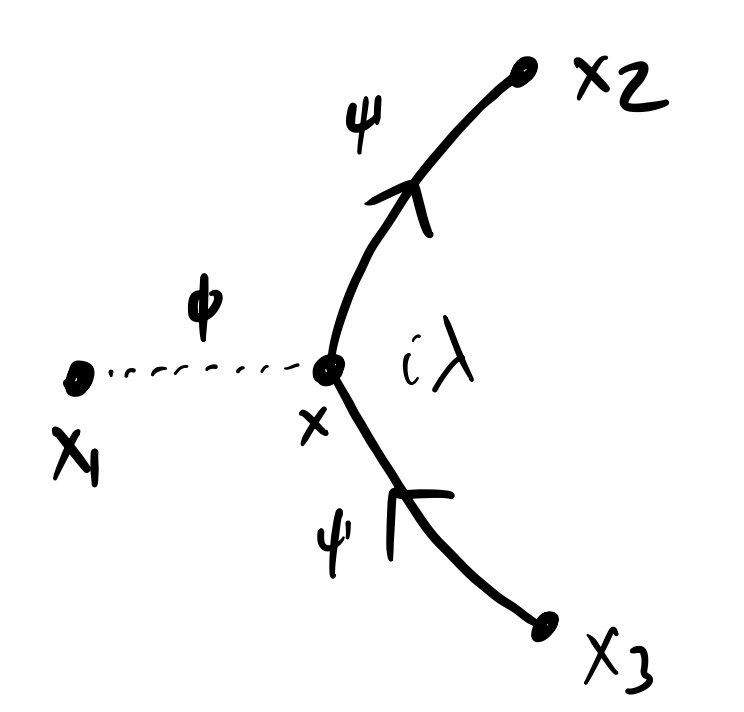
\includegraphics[scale=0.35]{Lectures/Images/lec6-xfeynman.png}
\end{center}

Or in momentum space:
\begin{equation}
    \avg{\phi_p\psi \bar{\psi}_{p'}} = i\lambda G_\phi(p)G_{\psi}(p + p')G_\psi(p') = i\lambda \frac{-i}{p^2 +M^2}\frac{-i}{\slashed{p} + \slashed{p}' + m}\frac{-i}{\slashed{p}' + m}
\end{equation}

\begin{center}
    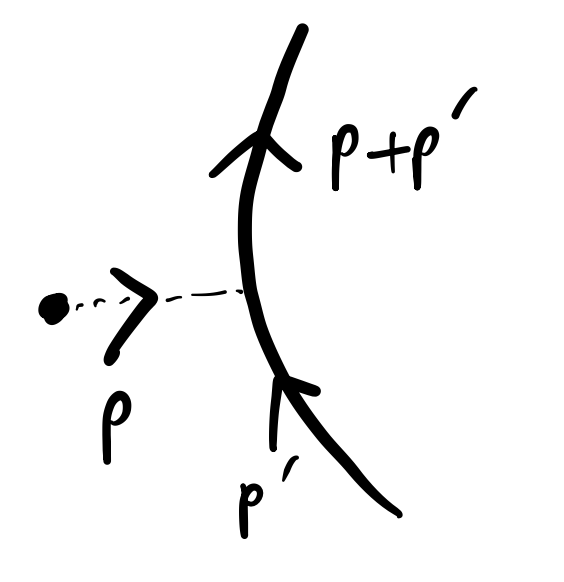
\includegraphics[scale=0.35]{Lectures/Images/lec6-pfeynman.png}
\end{center}


The amputated correlator $\avg{\phi_p\psi\bar{\psi}_{p'}}_{\text{amp}} = i\lambda\II$ will be related through LSZ to the 1$\to$2 S-matrix, namely the decay of a scalar particle into an electron/positron pair. When is the scalar particle unstable? If we imagine this in the rest frame of the scalar particle, this process requires $M > 2m$ (to produce the fermion and its antiparticle pair, plus giving the two kinetic energy) - when this condition is met $\phi$ is unstable, allowing for $\phi \to e^-e^+$, with decay rate $\Gamma \sim \lambda^2$ (which you will compute in PS4). 

\begin{center}
    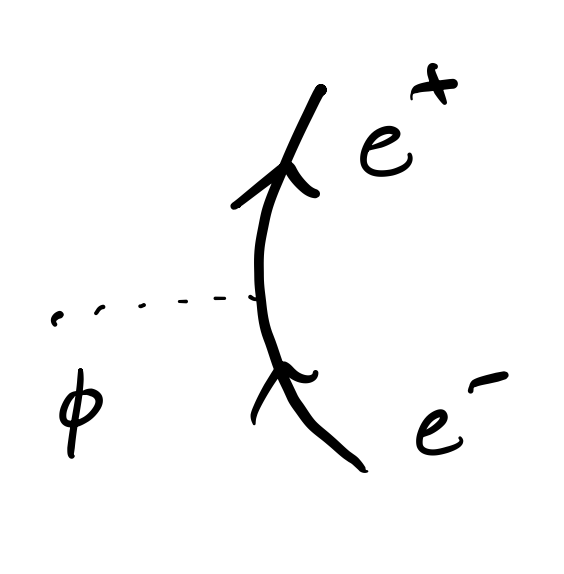
\includegraphics[scale=0.35]{Lectures/Images/lec6-scattering.png}
\end{center}

The decay rate also enters into the self-energy of the scalar, from which it is evident that $\Gamma \sim \lambda^2$.

\begin{center}
    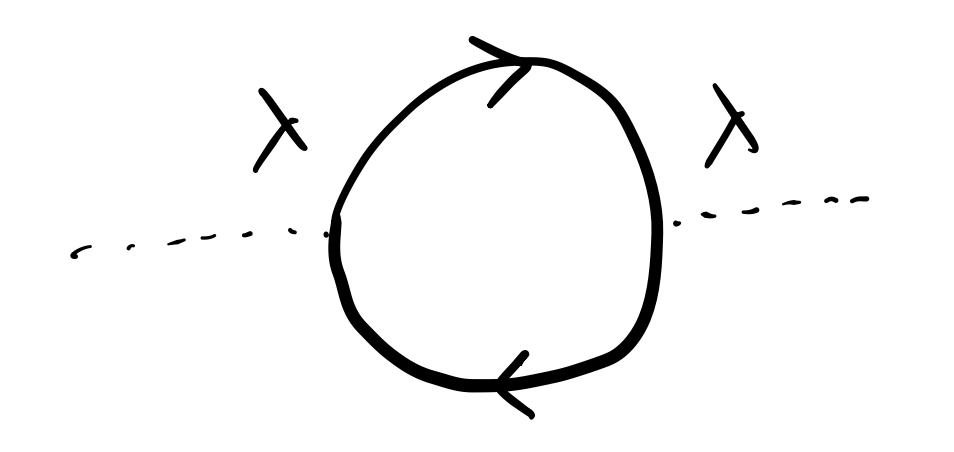
\includegraphics[scale=0.35]{Lectures/Images/lec6-selfenergy.png}
\end{center}

\subsection{Heavy Scalar Limit of Yukawa Theory - Fermi EFT}
Taking the limit where $M$ is huge (larger beyond all other energy scales), we can study its effects by integrating it out. Our full QFT has the generating functional:
\begin{equation}
    Z = \int \mathcal{D}\psi^\dag \mathcal{D}\psi \mathcal{D}\phi e^{i\int \bar{\psi}(i\slashed{p} - m)\psi + \lambda \phi \bar{\psi}\psi - \frac{1}{2}\phi(\p^2 + M^2)\phi}
\end{equation}
Note that if we just look at the $\phi$s (i.e. the $\phi$-sector), this is actually just a Gaussian theory! In our ultra-heavy limit, the mass energy is much greater than the kinetic term, so we neglect $\frac{1}{2}\phi(\p^2)\phi$. Thus, writing the $\phi$-part as:
\begin{equation}
    -\frac{1}{2}(\phi - \frac{\lambda}{M^2}\bar{\psi}\psi)M^2\left(\phi - \frac{\lambda}{M^2}\bar{\psi}\psi\right) + \frac{1}{2}\frac{\lambda}{M^2}\bar{\psi}\psi \bar{\psi}\psi
\end{equation}
Thus writing $\tilde{\phi} = (\phi - \frac{\lambda^2}{M^2}\bar{\psi}\psi)$, the above becomes:
\begin{equation}
    Z = \left(\int \mathcal{D}\tilde{\phi} e^{-\frac{1}{2}\tilde{\phi}M\tilde{\phi}}\right)\int \mathcal{D}\psi^\dag \mathcal{D}\psi e^{i\int \bar{\psi}(i\slashed{p} - m)\psi + \frac{1}{2}\frac{\lambda^2}{M^2}\bar{\psi}\psi\bar{\psi}\psi}
\end{equation}
So we can see that the $\phi$ generated an effective 4-fermion interaction! Free fermions do not scatter, but we have the emergence of an interaction vertex, mediated by the $\phi$ particle (which creates an effective interaction $ig_{\text{eff}} = i\frac{\lambda^2}{M^2}$); we can picture this as:

\begin{center}
    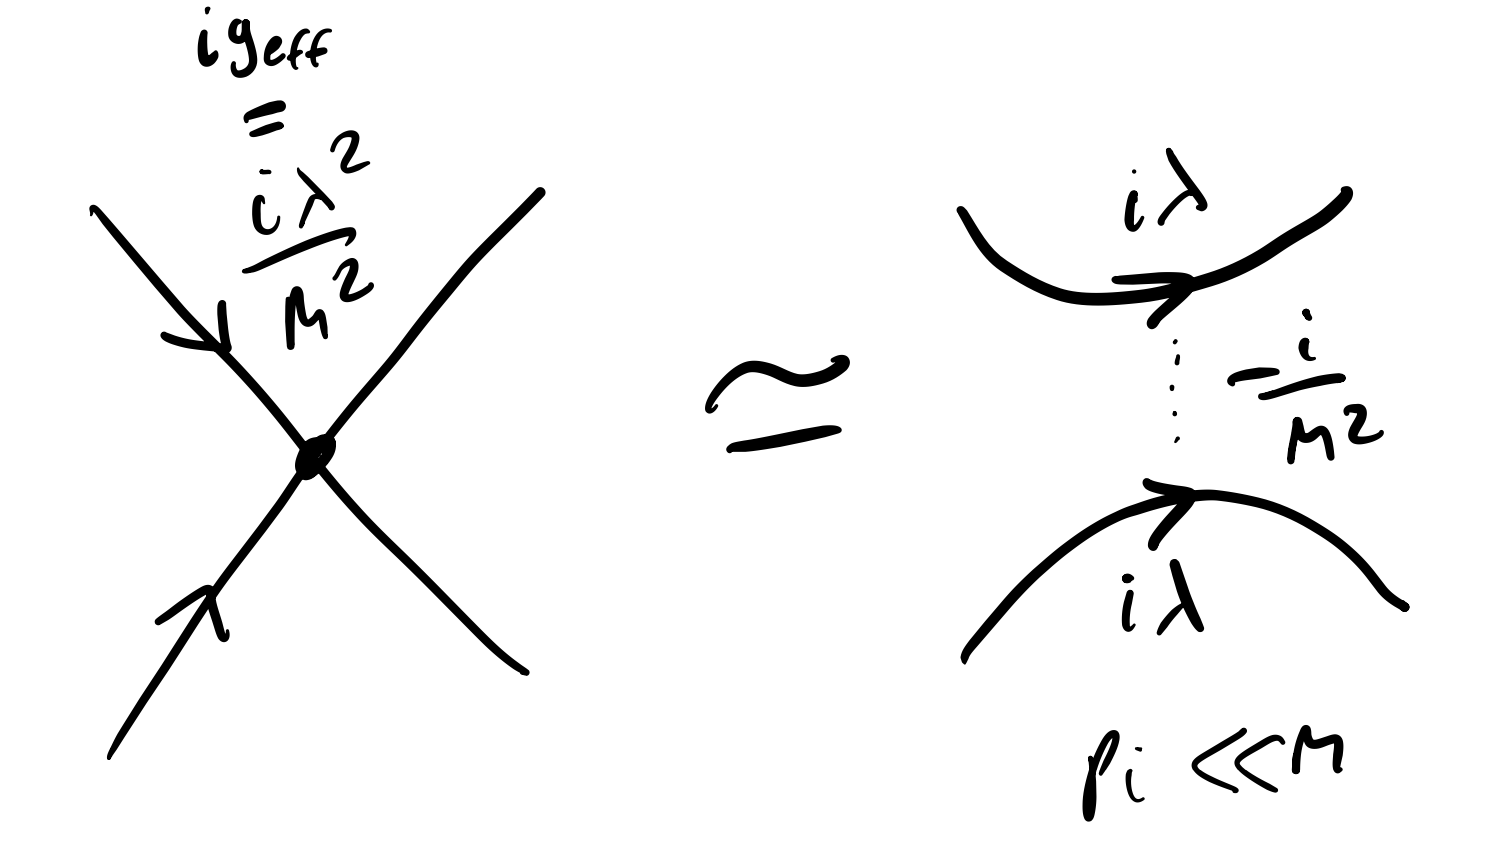
\includegraphics[scale=0.3]{Lectures/Images/lec6-effectiveinteraction.png}
\end{center}

This was the first effective theory considered - this is Fermi's effective field theory (EFT) of weak interactions, to explain $\beta$-decay. Radioactive materials emit electrons from time to time, with more specifically a neutron decaying into an electron, proton, and neutrino. This requires a 4-fermion interaction $g\bar{\psi}_1\psi_2\bar{\psi}_3\psi_4$. The microscopics of the theory came later, but the first try at explaining this phenomena was this EFT.

\begin{center}
    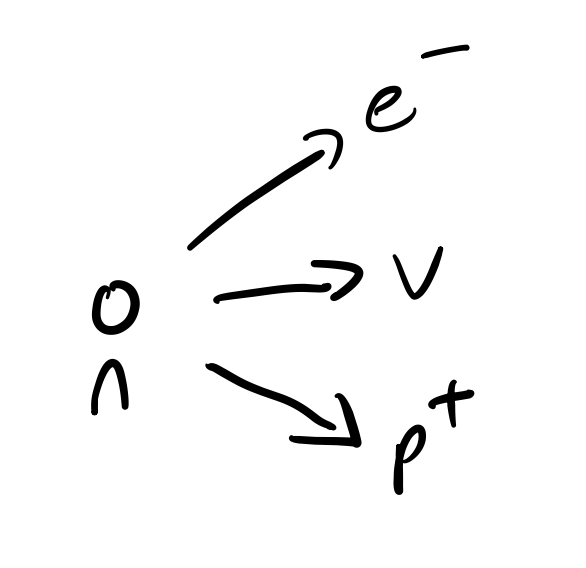
\includegraphics[scale=0.3]{Lectures/Images/lec6-neutrondecay.png}
\end{center}

This $\psi\bar{\psi}\psi\bar{\psi}$ interaction is irrelevant, or non-renormalizable. This is an energy that shrinks at small energies/IR and grows at high energies/UV. It is thus not UV complete, and cannot be the microscopic description of the theory. For us, the ``UV completion'' is the Yukawa theory (in Fermi's case it was a little more complicated, e.g. with Gauge fields). This effective interaction can be thought of as a force between particles (here the fermions $e^-, e^+$) that is mediated by the mysterious heavy particle. We can literally write this interaction as a potential:
\begin{equation}
    \begin{split}
        H_{\text{int}} &= -\frac{\lambda^2}{2M^2}\int d^4x \bar{\psi(x)}\psi(x)\bar{\psi}(x)\psi(x)
        \\ &=\int d^4xd^4y \bar{\psi(x)}\psi(x)V(x-y)\bar{\psi}(y)\psi(y)
    \end{split}
\end{equation}
where:
\begin{equation}
    V(x-y) = -\frac{\lambda^2}{2M^2}\delta^4(x-y)
\end{equation}
is a local interaction. In the problem set, you will find that this interaction is not a delta function (it is just sharply peaked), but in this extreme limit we currently consider, it is completely local. Given a particle at $x'$, because $V < 0$, it is energetically favourable to place another particle nearby. The Yukawa potential allows scalar particles to generate attractive interactions between fermions.

A final comment; if we spell out $\bar{\psi}\psi$, we find:
\begin{equation}
    \bar{\psi}\psi \sim b^\dag b + d^\dag d.
\end{equation}
Thus, all the particles - both fermions and anti-fermions attract each other. Phrased another way:
\begin{equation}
    H_{\text{int}} \sim \int_{xx'}(n_b + n_d)_xV(x - x')(n_b + n_d)_{x'}
\end{equation}
This is \emph{not} how we see electrons behave (which of course repulse), which indicates to us that the scalar particle is not what mediates the force between electrons. Instead, in QED we have that the force between electrons is mediated by the photon/gauge field\footnote{This wins out over the scalar mediation, as the photon is massles (and hence can mediate a long-range interaction), compared to the scalar mediated interaction which is short-ranged} $A_\mu$. This does not couple $\bar{\psi}, \psi$, but rather couples the current $j^\mu = \bar{\psi}\gamma^\mu \psi$, and in particular:
\begin{equation}
    \bar{\psi}\gamma^0 \psi = b^\dag b - d^\dag d
\end{equation}
So in QED:
\begin{equation}
    H_{\text{int}} \sim -\int_{xx'}(n_b - n_d)_xV(x - x')(n_b - n_d)_{x'}
\end{equation}
which means particles of the same charge repel, and particles of opposite charge attract. We will return to this soon!

Q (from me): Is it possible to look at the opposite limit where $2m \gg M$ (i.e. where the fermions are much heavier than the scalar), and integrate out the fermions, since the fermion subsector of the Yukawa Lagrangian is also Gaussian?

A (Luca): Yes; but note that this generates diagrams to all powers/orders of $\phi$, so is quite complicated. But, this is what people do, e.g., when they do quantum monte carlo simulations, because fermions are in general difficult to simulate (presumably due to sign problems).
\section{Vector Fields and QED I - Classical E\&M, Maxwell Equations, Gauge Invariance, Coupling to Matter}

We move to the next nontrivial representation of the Lorentz group! Namely the $(\frac{1}{2}, \frac{1}{2})$ representation with spin-1, which transforms like a 4-vector. You have already encountered this previously in the form of the photon in E\&M. Today we will start from classical electromagnetism, and derive the Maxwell equations from an action principle.

\subsection{The Maxwell Equations}
We can write Maxwell's equations compactly in a Lorentz covariant way:
\begin{equation}\label{eq:maxwell1}
    \p_\mu F^{\mu\nu} = j^\nu
\end{equation}
\begin{equation}\label{eq:maxwell2}
    \e^{\mu\nu\lambda\rho}\p_\nu F_{\lambda \rho} = 0
\end{equation}
with $F_{\mu\nu} = -F_{\nu\mu}$ the antisymmetric Maxwell stress tensor, with $\frac{4 \cdot 3}{2} = 6$ components; 3 for the electric and 3 for the magnetic field. In particular:
\begin{equation}
    \begin{split}
        F_{0i} &= E_i
        \\ F_{ij} &= -\e_{ijk}B^k
    \end{split}
\end{equation}
Indeed, let's see that this compact form of the Maxwell equations indeed reproduces the more familiar form. Looking at Eq. \eqref{eq:maxwell1} for $\nu = 0$:
\begin{equation}
    \rho = j^0 = \p_i F^{i0} = -\p_i F^{0i} = (-1)^2 \p_i F_{01} = \nabla \cdot \v{E}
\end{equation}
which is Gauss' Law. For $\nu = i$:
\begin{equation}
    j^i = \p_0 F^{0i} + p_j F^{ji} = -\p_0 E_i - \e_{ijk}\p_j B_k = -\dot{E}_i + \e_{ijk}\p_j B_k
\end{equation}
or if we look at all components:
\begin{equation}
    \v{j} = -\dot{\v{E}} + \nabla \times \v{E}
\end{equation}
which is Ampere's Law.

Now looking at Eq. \eqref{eq:maxwell2} for $\mu = 0$:
\begin{equation}
    0 = \e^{ijk}\p_i F_{jk} = -\e^{ijk}\e_{jkl}\p_i B^l = -\delta^{i}_l \p_i B^l \propto \nabla \cdot \v{B} \implies 0 = \nabla \cdot \v{B}
\end{equation}
which gives the Magnetic Gauss' law. Finally, for $\mu = i$:
\begin{equation}
    0 = \e^{i\nu \lambda \rho}\p_\nu F_{\lambda \rho} = \e^{i0jk}\p_0 F_{jk} + \e^{ij0k}\p_j F_{0k} = \e^{ijk}\e_{jkl}\p_0 B^l + 2\e^{ijk}\p_j E_k = 2\delta^{i}_l \p_0 B^l + 2\e^{ijk}\p_j E_k \implies \dot{\v{B}} + \nabla \times \v{E} = 0
\end{equation}
note in the second equality we have used the requirement that one of the indices be time (as the Levi-Civita tensor is only nonzero when all four indices are different.) The last equation is Faraday's Law, and so we have reproduced the four familiar versions of Maxwell's Law.

One can check that $F_{\mu\nu}$ transforms like a tensor under Lorentz transformations:
\begin{equation}
    F_{\mu\nu}(x) \to \Lambda_{\mu}^{\sp\alpha}\Lambda_{\nu}^{\sp\mu}F_{\alpha\beta}(\Lambda^{-1}x)
\end{equation}
Intuitively, under a boost charges become currents and so we transform between the tensor components. Writing things in terms of the electromagnetic tensor makes lorentz invariance manifest, provided $j^\mu$ is a Lorentz 4-vector. Another feature - observe that the current $j^\mu$ also has to be conserved:
\begin{equation}
    \p_\mu j^\mu = \p_\mu \p_\nu F^{\mu\nu} = 0
\end{equation}
where we conclude things are zero because the derivatives are symmetric while $F^{\mu\nu}$ is antisymmetric. This property is very reminiscent of Noether's theorem - it gives us the intuition that the electric/magnetic fields will want to couple to field theories with a $U(1)$ conservation law.

\subsection{Action Principle for Free Maxwell Theory}
Writing things in terms of $\v{E}, \v{B}$ is not great because they transform into each other under Lorentz boosts (the equations thus do not look Lorentz invariance). There is a further issue. The Magnetic Gauss' Law $\nabla \cdot \v{B} = 0$ implies that, locally, $\v{B}$ is a curl:
\begin{equation}
    \v{B} = \nabla \times \v{A}
\end{equation}
or equivalently:
\begin{equation}
    F_{ij} = \p_i A_j - \p_j A_i.
\end{equation}
Similarly, Faraday's Law says:
\begin{equation}
    0 = \nabla \times (\v{E} + \dot{\v{A}})
\end{equation}
which tells us that locally, $\v{E} + \dot{\v{A}}$ is a gradient:
\begin{equation}
    \v{E} + \dot{\v{A}} = \nabla A_0
\end{equation}
or:
\begin{equation}
    F_{i0} = \p_i A_0 - \p_0 A_i
\end{equation}
In summary:
\begin{equation}
    F_{\mu\nu} = \p_\mu A_\nu - \p_\nu A_\mu
\end{equation}
Writing the field strength in this way, Eq. \eqref{eq:maxwell2} is now automatic:
\begin{equation}
    \e^{\mu\nu\lambda\rho}\p_\nu F_{\lambda\rho} = 2\e^{\mu\nu\lambda\rho}\p_\nu\p_\lambda A_\rho = 0
\end{equation}
where we conclude that this vanishes as $\e^{\mu\nu\lambda\rho}$ is antisymmetric while $\p_\nu\p_\lambda$ is symmetric. Where does Eq. \eqref{eq:maxwell1} come from in this perspective? We view it as arising as the equation of motion of an action. So, let's try to find an action principle for Maxwell's equations. Let's start without charged matter; $\p_\mu F^{\mu\nu} = 0$. Schematically, it looks like:
\begin{equation}
    0 = \p_\mu F^{\mu\nu} \sim \p\p A \sim \text{Klein-Gordon} \implies \mathcal{L} = \frac{1}{2}A\p\p A
\end{equation}
Let's be a little more precise. There are only two possible index contractions:
\begin{enumerate}[(a)]
    \item $\p_\mu A_\nu \p^\mu A^\nu$
    \item $\p_\mu A^\mu \p_\nu A^\nu$
    \item There is an apparent final contender $\p_\mu A_\nu \p^\nu A^\mu$, but we can integrate by parts to swap derivatives, which makes this term equivalent to (b).
\end{enumerate}
Thus, we have:
\begin{equation}
    S = \frac{1}{2}a(\p_\mu A_\nu)^2 + b(\p_\mu A^\mu)^2
\end{equation}
so then the variation becomes:
\begin{equation}
    \delta S = -\int a \p_\mu A_\nu \p^\mu \delta A^\nu + b \p_\mu A^\mu \p_\nu \delta A^\nu
\end{equation}
now integrating by parts to isolate the variation:
\begin{equation}
    \delta S = \int \delta A_\nu [a\p_\mu \p^\mu A_\nu + b\p^\mu \p_\nu A_\mu]
\end{equation}
Hence $\delta S = 0$ for any variation $\delta A_\nu$ forces the term in brackets to be zero, i.e.:
\begin{equation}
    a\p_\mu(\p^\mu A^\nu) + b\p_\mu (\p^\nu A^\mu) = 0
\end{equation}
This indeed yields the equation of motion:
\begin{equation}
    0 = \p_\mu F^{\mu\nu} = \p_\mu (\p^\mu A^\nu - \p^\nu A^\mu)
\end{equation}
in the case that $b = -a$. Thus, the action that produces Eq. \eqref{eq:maxwell1} is:
\begin{equation}
    S = -\frac{1}{2}\int (\p_\mu A_\nu)^2 - (\p_\mu A^\mu)^2
\end{equation}
Integrating by parts the second term to swap the derivatives $\p_\mu A^\mu \p_\nu A^\nu = \p_\nu A^\mu \p_\mu A^\nu$, we obtain:
\begin{equation}
    S = -\frac{1}{2}\int \p^\mu A^\nu(\p_\mu A_\nu - \p_\nu A_\mu) = -\frac{1}{2}\int \p^\mu A^\nu F_{\mu\nu}
\end{equation}
Since $\p^\mu A^\nu$ is contracted with an antisymmetric tensor, we can replace it with its antisymmetric part, which is just the maxwell tensor again:
\begin{equation}
    \p^\mu A^\nu \stackrel{\text{antisymmetric}}{=} \frac{1}{2}(\p^\mu A^\nu - \p^\nu A^\mu) = \frac{1}{2}F^{\mu\nu}
\end{equation}
and thus:
\begin{equation}
    S = -\frac{1}{4}\int d^4x F_{\mu\nu}F^{\mu\nu}
\end{equation}
we have thus obtained an action principle for the Maxwell equations with no matter.

\subsection{Adding Charged Matter}
What we really want is not $\p_\mu F^{\mu\nu} = 0$, but rather $\p_\mu F^{\mu\nu} = j^\nu$, or equivalently:
\begin{equation}
    \p_\mu F^{\mu\nu} - j^\nu = 0
\end{equation}
We already have the first term from $\delta S$ that we constructed above, we just need another term in the action for which $\delta S'/\delta A_\nu$ gives the current. We need:
\begin{equation}
    \delta S' = -\int \delta A_\nu j^\nu \implies S' = -\int A_\nu j^\nu
\end{equation}
and thus the total action is:
\begin{equation}
    \boxed{S[A] = -\int d^4x \frac{1}{4}(F_{\mu\nu})^2 + A_\mu j^\mu}
\end{equation}
with the additional equation:
\begin{equation}
    \boxed{F_{\mu\nu} = \p_\mu A_\nu - \p_\nu A_\mu}
\end{equation}
from these we can reproduce everything from classical electromagnetism.

\subsection{Gauge Invariance}
In addition to Lorentz and translation symmetry, the above theory has a strange ``symmetry'' known as Gauge invariance (not a true symmetry, just an invariance of the action). This symmetry acts on the vector field as follows:
\begin{equation}
    A_\mu(x) \to A_\mu(x) + \p_\mu \lambda(x)
\end{equation}
where $\lambda(x)$ is an \emph{arbitrary} scalar function of spacetime. How do we see that this indeed leaves the action invariant? Indeed:
\begin{equation}
    F_{\mu\nu} = \p_\mu A_\nu - \p_\nu A_\mu \to \p_\mu A_\nu - \p_\mu A_\mu - (\p_\mu \p_\nu \lambda - \p_\nu \p_\mu \lambda) = \p_\mu A_\nu - \p_\mu A_\mu = F_{\mu\nu}
\end{equation}
where the term in brackets vanishes due to the symmetry of the derivatives. Writing the field strength as a curl hence picks up a kind of redundancy. Moreover, we can see that the second part of the action is also invariant:
\begin{equation}
    -\int A_\mu j^\mu \to -\int A_\mu j^\mu + \p_\mu \lambda j^\mu \stackrel{\text{IBP}}{=} -\int A_\mu j^\mu - \lambda \p_\mu j^\mu = -\int A_\mu j^\mu
\end{equation}
where in the last equality we use that $\p_\mu j^\mu = 0$, as we couple to conserved currents.

This is a bit different from a symmetry - it should be thought of as a redundancy of our description. Several different choices of $A_\mu$ can give rise to the same physics. Loosely, we can think of it as one ``component'' of $A_\mu$ does not appear in the action. One can fix this redundancy by choosing/fixing a gauge.
\begin{enumerate}[(a)]
    \item $A_0 = 0$ (Temporal gauge)
    \item $\nabla \cdot \v{A} = 0$ (Coloumb gauge)
    \item $\p_\mu A^\mu = 0$ (Lorenz gauge)
\end{enumerate}
To understand what is left of the dynamics of our system, let us pick one gauge and then study what is left. For now, we will choose the Coloumb gauge, which is one that you may have already played with in your E\&M class (it is a useful choice for working with electrostatics). Let's see the impact of this choice on the action.
\begin{equation}
    \begin{split}
        S = -\frac{1}{4}\int F^2 &= -\frac{1}{4}\int -2F_{0i}F^{0i} - F_{ij}F^{ij} 
        \\ &= \int \frac{1}{2}(\p_0 A_i - \p_i A_0)(\p_0 A_i - \p_i A_0) + \frac{1}{2}\p_i A_j(\p_i A_j - \p_j A_i)
        \\ &= \int \frac{1}{2}(\p_0 A_i)^2 + \frac{1}{2}(\p_i A_0)^2 - \frac{1}{2}(\p_i A_j)^2
        \\ &= \int \frac{1}{2}A_i(-\p_0^2 + \p_j^2)A_i - \frac{1}{2}A_0\nabla^2 A_0
    \end{split}
\end{equation}
where in the third line we note that the use of IBP gives $\p_i A_i = \nabla \cdot \v{A} = 0$ by our choice of gauge for some of the terms. We see here that the equation of motion for $A_0$ is:
\begin{equation}
    \nabla^2 A^0 = j^0
\end{equation}
i.e. $A^0$ in this gauge is not a propagating degree of freedom. It's fixed by the charge density profile.

To review; we started with $A_\mu$ which has 4 degrees of freedom. This was a bit redundant, because the action was invariant under a transformation $A_\mu \to A_\mu + \p_\mu \lambda$. We fixed a gauge (Coloumb) so that we had $A_\mu, \nabla \cdot \v{A} = 0$, i.e. we now have 3 degrees of freedom. This gave an additional constraint, namely $A^0$ being fixed by $j^0$. Hence by the end we were left with 2 degrees of freedom. This is what we expected; 2 is the DoFs for a massless field (the 2 helicities), as you saw on a former homework.

\subsection{Coupling Maxwell to Dirac}
So, we have our Maxwell theory:
\begin{equation}
    S = -\int d^4x \frac{1}{4e^2}(F_{\mu\nu})^2 + A_\mu j^\mu
\end{equation}
where we have renormalized $A \to eA$ implying $\p_\mu F^{\mu\nu} = ej^\nu$. It needs to be coupled to a conserved current $\p_\mu j^\mu = 0$. Dirac fermions have precisely such a current. Namely, with the action:
\begin{equation}
    S = \int \bar{\psi}(i\slashed{\p} - m)\psi
\end{equation}
we have the symmetry $\psi \to e^{i\lambda}\psi$ which the Noether procedure gives the current:
\begin{equation}
    j^\mu = \bar{\psi}\gamma^\mu \psi
\end{equation}
The full Maxwell + matter (Dirac) action is thus:
\begin{equation}
    S = \int \bar{\psi}(i\slashed{\p} - m)\psi - A_\mu \bar{\psi}\gamma^\mu \psi - \frac{1}{4e^2}(F_{\mu\nu})^2
\end{equation}
Something we can do in this theory (and something that one often does) is to package the interaction $A_\mu \bar{\psi}\gamma^\mu \psi$ into the derivative:
\begin{equation}
    \boxed{S = \int \bar{\psi}(i\slashed{D} - m)\psi- \frac{1}{4e^2}(F_{\mu\nu})^2}
\end{equation}
where we have defined a covariant derivative:
\begin{equation}
    D_\mu = \p_\mu + iA_\mu
\end{equation}
so then:
\begin{equation}
    \slashed{D} \psi = \gamma^\mu(\p_\mu + iA_\mu)\psi = \slashed{\p}\psi + iA_\mu \gamma^\mu \psi
\end{equation}

So, we have our action for QED! We have our Dirac theory, our Maxwell theory, and then our interaction, which leads to many interesting effects. The presence of this interaction makes the theory unsolvable, but quite interesting and subtle.

We can ask why did we package the derivative in this strange way. We do this because this coupled theory still retains the gauge invariance of Maxwell theory. Namely, the action is invariant under the transformations:
\begin{equation}
    \begin{split}
        A_\mu &\to A_\mu + \p_\mu \lambda(x)
        \\ \psi &\to e^{i\lambda(x)}\psi
    \end{split}
\end{equation}
Interestingly, this is still an invariance of the action when $\lambda(x)$ is a fully arbitrary (real) scalar function of spacetime. Let's check that this is true. The $F^2$ invariance carries over from the maxwell theory, and $m\bar{\psi}\psi$ is also easy to see (the $e^{\pm i\lambda}$s cancel). What about the kinetic term $\bar{\psi}i\slashed{D}\psi$? Well, looking at how the covariant derivative transforms:
\begin{equation}
    \begin{split}
        D_\mu \psi = \p_\mu \psi + iA_\mu \psi &\to \p_\mu (e^{i\lambda(x)}\psi) + iA_\mu e^{i\lambda(x)}\psi - i\p_\mu \lambda e^{i\lambda(x)}\psi
        \\ &= i\p_\mu \lambda e^{i\lambda}\psi - i\p_\mu \lambda e^{i\lambda}\psi + e^{i\lambda}\p_\mu \psi + e^{i\lambda}iA_\mu \psi = e^{i\lambda(x)}D_\mu \psi
    \end{split}
\end{equation}
Thus we see that $D_\mu \psi \to e^{i\lambda(x)}D_\mu\psi$, which is why we wanted to package things this way to get this easy transformation rule. Thus the kinetic term is easily seen to be invariant:
\begin{equation}
    \bar{\psi}\gamma^\mu D_\mu \psi \to \bar{\psi}e^{-i\lambda}e^{i\lambda}\gamma^\mu D_\mu \psi = \bar{\psi}\gamma^\mu D_\mu \psi
\end{equation}
Thus - as in the case with pure Maxwell theory, it is still true that the photon carries less degrees of freedom than as it first appears. The degrees of freedom available here will be the 2 helicities of the photon and the Dirac field.

Note; here we have chosen to couple Dirac with Maxwell, but we can choose any theory with a conserved current; for example the scalar theory:
\begin{equation}
    S = \int (\p\phi)^2 + (\p\phi)^4
\end{equation}
has the shift symmetry $\phi \to \phi + c$. In this model the covariant derivative will look different. We have the gauge transformations:
\begin{equation}
    \begin{split}
        \phi &\to \phi + \lambda(x)
        \\ A_\mu &\to A_\mu - \p_\mu \lambda(x)
    \end{split}
\end{equation}
So then the correct way to make a covariant derivative is:
\begin{equation}
    D_\mu \phi = \p_\mu \phi - A_\mu \to \p_\mu \phi - A_\mu
\end{equation}
So we have the action:
\begin{equation}
    S = -\int (D\phi)^2 + (D\phi)^4 + \frac{1}{4e^2}F^2
\end{equation}
which actually turns out to describe a superconductor! We won't discuss this in lecture in too much detail, but you may see it show up on a future homework.
\section{Electron Dipole Moment, Path Integral for Gauge Fields}
Last lecture, we found the QED action:
\begin{equation}
    S = \int d^4x \bar{\psi}(i\slashed{\p} - m)\psi + A_\mu \bar{\psi}\gamma^\mu \psi + \frac{1}{4e^2}(F_{\mu\nu})^2 = \int d^4x\bar{\psi}(i\slashed{D} - m)\psi - \frac{1}{4e^2}F^2
\end{equation}
where in the second equality we introduce the covariant derivative:
\begin{equation}
    D_\mu \psi = \p_\mu \psi + iA_\mu \psi
\end{equation}
which is useful because it makes the action manifestly gauge invariant (you can observe that under a $U(1)$ transformation, the covariant derivative only picks up a phase).

\subsection{Magnetic dipole of the electron}
We do not yet know how to treat the gauge fields at a quantum-mechanical level. But even before going there, we can already make some predictions, just via treating the gauge fields classically. Namely, the electron is not just a point charge, but it also couples to the magnetic field, and we will see the prediction for its magnetic moment come out of the QED action.

\begin{center}
    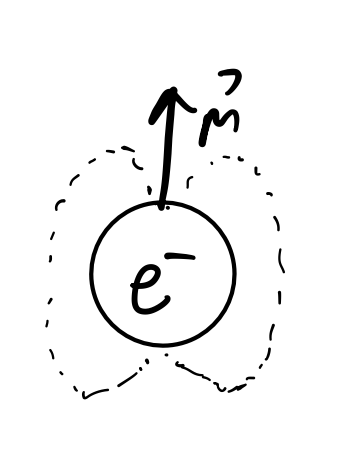
\includegraphics[scale=0.35]{Lectures/Images/lec8-emagmoment.png}
\end{center}

For a non-relativistic particle, we could consider a Zeeman coupling:
\begin{equation}
    H = \frac{(\v{p} + \v{A})^2}{2m} + \mu\v{B} \cdot \gv{\sigma}
\end{equation}
wherein the particle eigenstates $\ket{\v{p}, s = \pm}$ are based on the particle momenta $\v{p}$ and spin $s$. $\mu$ is the free parameter, which tells us the energy splitting between the two spin states (as a function of $B$):

\begin{center}
    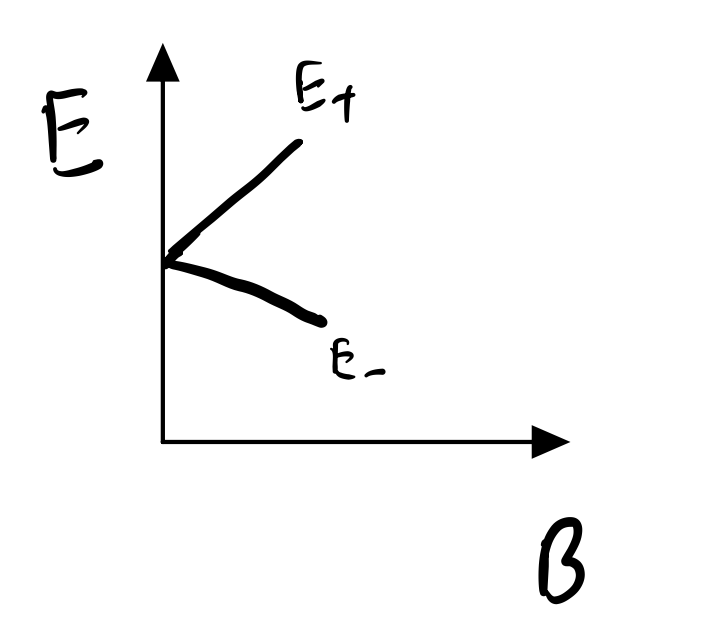
\includegraphics[scale=0.35]{Lectures/Images/lec8-energysplit.png}
\end{center}

Let's study the modified/gauged Dirac equation (the equation of motion in QED):
\begin{equation}
    0 = (i\slashed{D} + m)\psi
\end{equation}
and square it, in the way we derived Klein-Gordon equation from the regular dirac equation (This is how we derived the spectrum of free dirac fermions to be $E = \sqrt{p^2 + m^2}$):
\begin{equation}
    \begin{split}
        0 &= (i\slashed{D} + m)(-i\slashed{D} + m)\psi 
        \\ &= (\slashed{D}\slashed{D} + m^2)\psi
        \\ &= (\gamma^\mu\gamma^\nu D_\mu D_\nu + m^2)\psi
    \end{split}
\end{equation}
Now we write:
\begin{equation}
    \gamma^\mu\gamma^\nu = \frac{1}{2}\set{\gamma^\mu, \gamma^\nu} + \frac{1}{2}[\gamma^\mu, \gamma^\nu] = -\eta^{\mu\nu} - 2iS^{\mu\nu}
\end{equation}
with:
\begin{equation}
    S^{\mu\nu} = \frac{i}{4}[\gamma^\mu, \gamma^\nu]
\end{equation}
Thus:
\begin{equation}
    0 = (-D^2 - iS^{\mu\nu}2D_\mu D_\nu + m^2)\psi
\end{equation}
If we had no background ($A \to 0$), then the derivatives of $D_\mu D_\nu$ commute (hence symmetric), and its multiplied by an antisymmetric $S^{\mu\nu}$ and so the entire term vanishes. We are just left with the Klein-Gordon equation, as we expect. Since $2D_\mu D_\nu$ is contracted with $S^{\mu\nu}$, let us write it as:
\begin{equation}
    2D_{\mu}D_\nu \psi = (D_\mu D_\nu - D_\nu D_\mu)\psi
\end{equation}
where:
\begin{equation}
    D_\mu D_\nu \psi =  (\p_\mu + iA_\mu)(\p_\nu \psi + iA_\nu \psi) = \p_\mu \p_\nu \psi + i A_\nu \p_\mu \psi + i \p_\mu A_\nu \psi + i A_\mu \p_\nu \psi - A_\mu A_\nu \psi
\end{equation}
So the difference becomes (notice that most of the terms here are symmetric and cancel, with the exception of the $i\p_\mu A_\nu \psi$):
\begin{equation}
    [D_\mu, D_\nu]\psi = i(\p_\mu A_\nu - \p_\nu A_\mu)\psi = iF_{\mu\nu}\psi
\end{equation}
This is nice! Covariant derivatives are gauge invariant, and the thing we get out here is indeed a gauge invariant quantity.

Thus, returning to our equation of motion:
\begin{equation}
    0 = (-D^2 + S^{\mu\nu}F_{\mu\nu} + m^2)\psi
\end{equation}

Now, we want to study the energies of solutions to this equation when there is a magnetic field. We set $A_0 = 0$ and $\v{B} = \nabla \times \v{A}$. Only $F_{ij}$ are activated. What are the $S^{ij}$?:
\begin{equation}
    S^{ij} = \frac{i}{4}[\gamma^i, \gamma^j] = \frac{i}{4}\m{0 & \sigma^i \\ \bar{\sigma}^i & 0}\m{0 & \sigma^j \\ \bar{\sigma}^j & 0} - (i\leftrightarrow j) = \frac{i}{4}\m{[\sigma^i, \bar{\sigma}^j] & 0 \\ 0 & [\bar{\sigma}^i, \sigma^j]}
\end{equation}
Then looking at the relations that the Paulis satisfy:
\begin{equation}
    [\sigma^i, \sigma^j] = 2i\e^{ijk}\sigma_k
\end{equation}
we conclude:
\begin{equation}
    S^{ij} = \frac{1}{2}\e^{ijk}\m{\sigma^k & 0 \\ 0 & \sigma^k}
\end{equation}
Thus:
\begin{equation}
    S^{ij}F_{ij} = \frac{1}{2}\e^{ijk}\m{\sigma^k & 0 \\ 0 & \sigma^k} (\p_i A_j - \p_j A_i) = \m{\sigma^kB_k & 0 \\ 0 & \sigma^k B_k}
\end{equation}
So we have the full differential equation - to get the energies now all we need to do is fourier transform:
\begin{equation}
    E^2 = (\v{p} + \v{A})^2 + m^2 + \m{\gv{\sigma} \cdot \v{B} & 0 \\ 0 & \gv{\sigma} \cdot \v{B}}
\end{equation}
So the energy in the non-relativistic limit (wherein $m^2 \gg (\v{p} + \v{A})^2$) becomes:
\begin{equation}
    E = m\sqrt{1 + \frac{(\v{p} + \v{A})^2}{m^2} + \frac{1}{m^2} \m{\gv{\sigma} \cdot \v{B} & 0 \\ 0 & \gv{\sigma} \cdot \v{B}}} \approx m + \frac{(\v{p} + \v{A})^2}{2m} + \frac{1}{2m}\m{\gv{\sigma} \cdot \v{B} & 0 \\ 0 & \gv{\sigma} \cdot \v{B}}
\end{equation}
With the normalization of $A \to eA$ (the more familiar normalization from E\&M):
\begin{equation}
    E - m = \frac{(\v{p} + e\v{A})^2}{2m} + \frac{e}{2m}\gv{\sigma} \cdot \v{B}
\end{equation}
and thus:
\begin{equation}
    \boxed{\mu = \frac{e}{2m}}
\end{equation}
This is a nice and simple prediction, and one can compare it to experiments; we find:
\begin{equation}
    \mu = \frac{e}{2m}\cdot 1.0011597\ldots
\end{equation}
which is very close, but off! Why is it off? We treat the photon classically here, and there are quantum corrections. Pictorially, we can imagine that these corrections may look like (with the leftmost diagram the classical prediction):

\begin{center}
    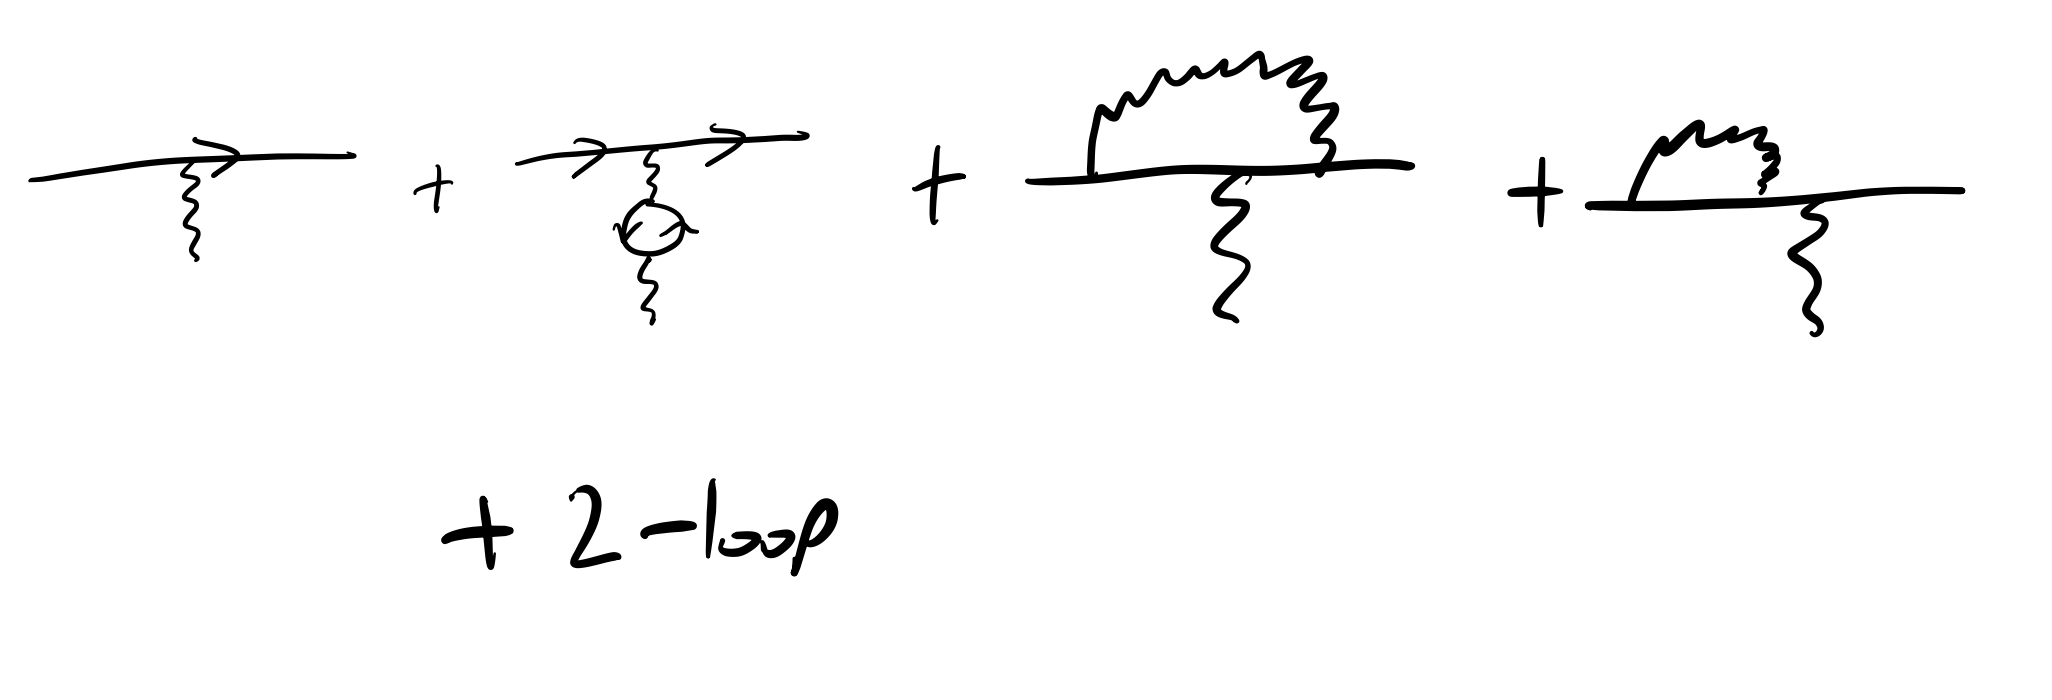
\includegraphics[scale=0.35]{Lectures/Images/lec8-mufeynmans.png}
\end{center}

The 1-loop corrections give the $0.00115$, and if you are braver and have a lot more time you can keep going, and the current agreement of theory and experiment is $10^{-13}$ (wow!) The dimensionless coupling in QED turns out to be small, which is why the perturbative expansion is useful here.

\subsection{Path Integral for Gauge Fields - First attempt}
Quantizing gauge fields is important not just for a more accurate prediction of the electron dipole, but in various aspects of particle and condensed matter physics. To do this, we jump straight to the path integral formulation. A good reference for this is Peskin 9.4, as well as Fradkin 9.5. We follow the approach by Fadeev and Popov approach. There are several advantages:
\begin{itemize}
    \item Path integrals! Much easier to calculate things
    \item Lorentz invariance is manifest
    \item Generalizes easily to quantization of non-abelian gauge fields
\end{itemize}
There are however alternatives you can read about, e.g. Gupta-Bleuler.

The naive guess for the path integral would be:
\begin{equation}
    Z = \int \mathcal{D}A_0 \mathcal{D}A_1 \mathcal{D}A_2 \mathcal{D}A_3 e^{iS_M[A]}
\end{equation}
with:
\begin{equation}
    S_M[A] = -\frac{1}{4}\int d^4x F^2
\end{equation}
and indeed this is not too far off. But it has some issues - namely due to gauge invariance. Loosely, gauge invariance tells us that there is a component of the gauge fields that does not enter into the action. So, one of the four integrals is over nothing. If this was it, it wouldn't be a huge problem, but there is a related larger problem; namely the kinetic term $\sim A\p\p A \sim AD A$ is not invertible (which is what we usually do to get the propagator). How do we see this? Well, looking at the Maxwell action:
\begin{equation}
    S_M[A] = -\frac{1}{4}\int_x F^2 = -\frac{1}{2}\int_x \p_\mu A_\nu (\p^\mu A^\nu - \p^\nu A_\mu) = \int_x A_\nu (\p^2 \eta^{\mu\nu} - \p^\nu \p^\mu)A_\mu
\end{equation}
and in momentum space this becomes:
\begin{equation}
    S_M[A] = -\int\frac{d^4p}{(2\pi)^4}A_\mu(-p)(p^2\eta^{\mu\nu} - p^\mu p^\nu) A_\nu(p)
\end{equation}
with $``D'' = (p^2\eta^{\mu\nu} - p^\mu p^\nu)$. Usually, we solve theories in the path integral formalism by coupling the theory to sources (say, $A_\mu J^\mu$) and complete the square to get something of the form $JD^{-1}J$. But here, $D$ is not invertible; indeed, we see this by acting $D$ on $p^\mu$:
\begin{equation}
    (p^2\eta^{\mu\nu} - p^\mu p^\nu)p^\mu = p^2p^\mu - p^2 p^\mu = 0
\end{equation}
i.e. $p^\mu$ is in the kernel of this matrix, and hence the matrix is not invertible. The underlying reason for this is due to the gauge invariance - ``Pure gauge configurations'' $A_\mu(x) = \p_\mu \lambda(x)$ have zero action and we should remove them/not be integrating over them.

A visual intuition; the space of gauge fields $A_\mu$ is large, but many of these fields are related via gauge transformations, and we integrate over these as well. The resolution is to choose a slice satisfying gauge fixing.

\begin{center}
    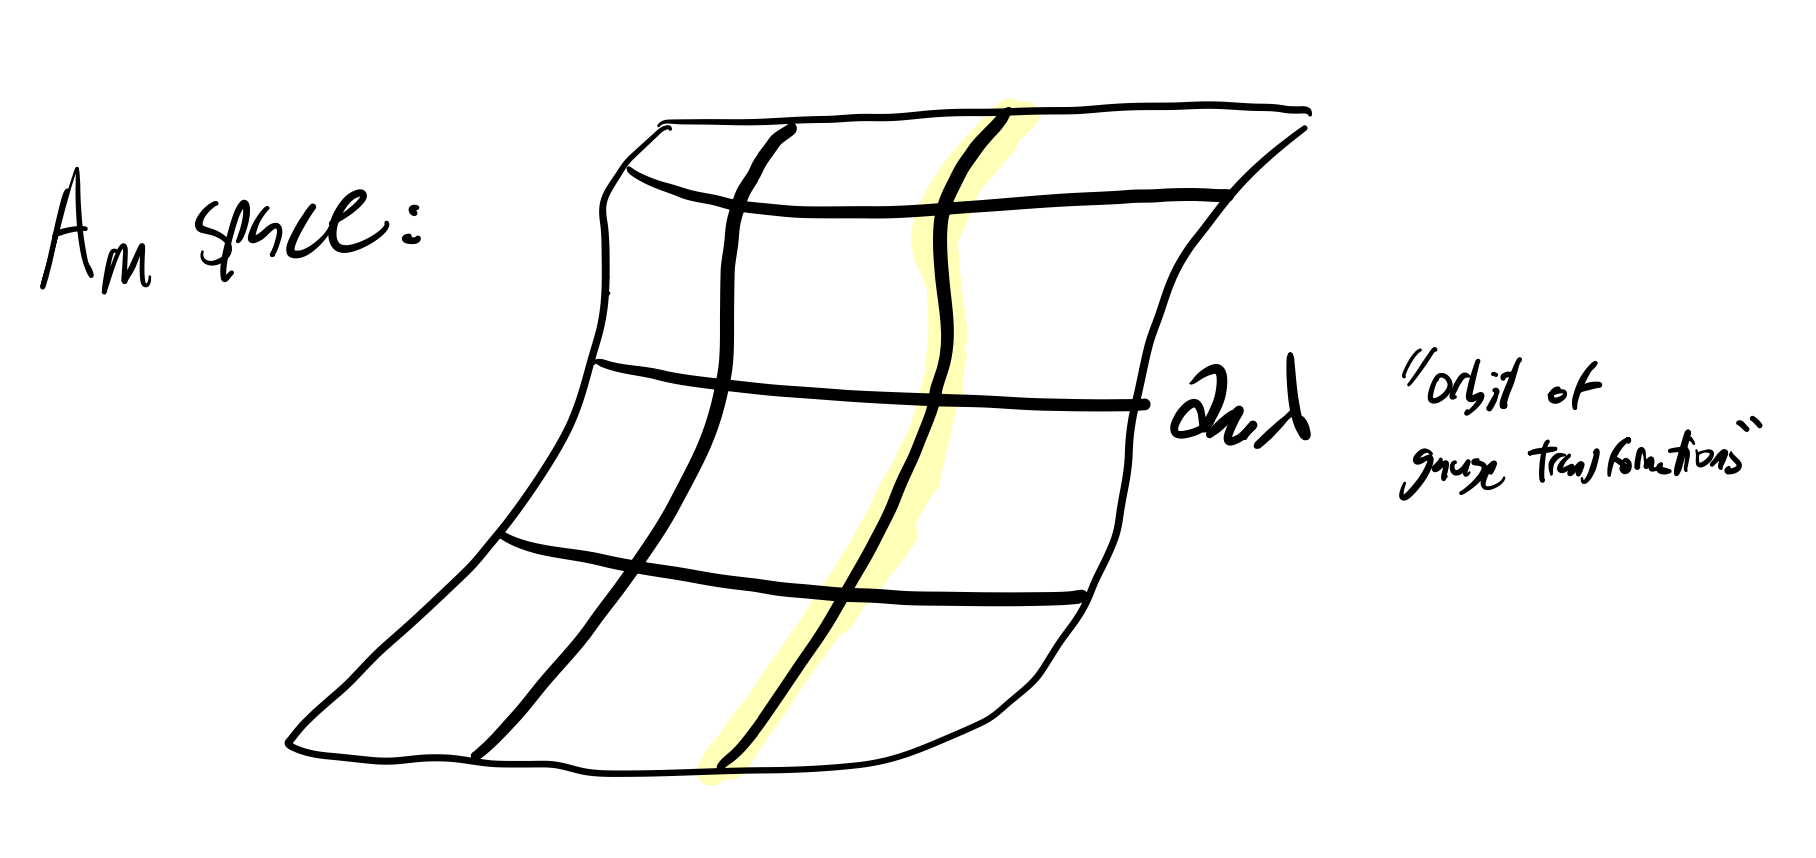
\includegraphics[scale=0.35]{Lectures/Images/lec8-gaugefields.png}
\end{center}

\subsection{Gauge Fixing in the Path Integral}
Consider a gauge-fixing condition:
\begin{equation}
    g(A_\mu) = \nabla \cdot \v{A} \;(\text{Coloumb}),\quad g(A_\mu) = \p_\mu A^\mu \;(\text{Lorenz}), \ldots
\end{equation}
After we fix a gauge, we can no longer relate different fields via gauge transformations, and we only integrate over ``true'' degrees of freedom. To this end would like to introduce something like $\delta(g(A))$ in the path integral. This will enforce that only configurations along a slice would enter the path integral.

To not mess things up, we will insert:
\begin{equation}
    1 = \int \mathcal{D}\lambda \delta(g(A_\lambda))\det \frac{\delta g(A_\lambda)}{\delta \lambda}
\end{equation}
where given $A_\mu$, $A^\lambda_\mu = A_\mu + \p_\mu \lambda$. The above expression is in analog to the single-variable function case, where $1 = \int dx \delta(f(x))\abs{f'(x)}$. So, our path integral then becomes:
\begin{equation}
    Z = \int \mathcal{D}\lambda \mathcal{D}A \delta(g(A^\lambda))\det \frac{\delta g(A_\lambda)}{\delta \lambda}e^{iS_M[A]}
\end{equation}
A comments; the path integral we started with is independent of any $g$, but since we insert 1, we don't introduce $g$ dependence (as should be the case, since we shouldn't expect fixing a gauge to change any of the physics). The introduction of this gauge fixing path integral will allow us to isolate the infinity/redundancy from the original path integral. Carrying on, note that the Maxwell equation is gauge invariant, so we can replace $A \to A_\lambda$. Therein only $A_\lambda$ appears in the integrand, so we can instead replace all variables with $A$, leaving the integrand $\lambda$-independent (note that the derivative term is also $\lambda$ independent, as we evaluate it at $A$ after taking the functional derivative):
\begin{equation}
    Z = \left(\int \mathcal{D}\lambda\right)\int \mathcal{D}A \delta(g(A))\left.\frac{\delta g(A^\lambda)}{\delta \lambda}\right|_A e^{iS_M[A]}
\end{equation}
Thus we have isolated the integral $\int \mathcal{D}\lambda$ over gauge orbits (that gives a factor of infinity) in a way that we can manifestly see it does nothing. Now we have an integral over $A$ with a delta function, which picks out a ``slice'' in gauge field space.

Now, this doesn't quite look like our regular Gaussian path integral, so we may have cause for worry. We will deal with this $\delta(g(A))$ by averaging over carefully chosen gauges. We consider:
\begin{equation}
    g_\omega(A) = \p_\mu A^\mu - \omega(x)
\end{equation}
the Lorenz gauge plus a function of spacetime. We average over these gauges with Gaussian weight:
\begin{equation}
    e^{i \int d^4x \frac{\omega^2(x)}{2\xi}}
\end{equation}
This trick will produce a Gaussian path integral!
\begin{equation}
    Z = \int \mathcal{D}A\mathcal{D}\omega e^{-i\int \frac{\omega^2(x)}{2\xi}}\delta(\p_\mu A^\mu - \omega)\det(\p^2)e^{-\frac{i}{4}\int_x F^2}
\end{equation}
An aside; the $\det(\p^2)$ term becomes much more interesting in the context of Non-Abelian gauge theories, as it then retains some dependence on $A$. Now, the $\omega$ integral is easy to evaluate, because we have a $\delta$ function fixing it:
\begin{equation}
    Z = \int \mathcal{D}Ae^{-i\int_x \frac{1}{4}F^2 + \frac{1}{2\xi}(\p_\mu A^\mu)^2}
\end{equation}
So what was the effect of all of this? We get an updated action:
\begin{equation}
    S = -\int d^4x \frac{1}{4}F^2 + \frac{1}{2\xi}(\p_\mu A^\mu)^2
\end{equation}
What's the point of doing this? Now, the kinetic term turns out to be invertible! Fourier transforming:
\begin{equation}
    S = -\int \frac{d^4p}{(2\pi)^4}A_\mu(-p)(\eta^{\mu\nu}p^2 - p^\mu p^\nu(1 - \frac{1}{\xi}))A_\nu(p)
\end{equation}
Let's find an inverse of:
\begin{equation}
    D^{\mu\nu} = \eta^{\mu\nu}p^2 - p^\mu p^\nu(1 - \frac{1}{\xi})
\end{equation}
via guessing; we want units of inverse $p^2$ and we want it to be Lorentz covariant with two indices, so our general guess is:
\begin{equation}
    (D^{-1})_{\mu\nu} = \frac{1}{p^2}(\eta_{\mu\nu} + \alpha\frac{p_\mu p_\nu}{p^2})
\end{equation}
Multiplying this out:
\begin{equation}
    (D^{-1})^{\mu\nu}D_{\nu\lambda} = (\eta^{\mu\nu} + \alpha\frac{p^{\mu}p^\nu}{p^2})(\eta_{\nu\lambda} - \frac{p_\nu p_\lambda}{p^2}(1 - \frac{1}{xi})) = \delta^{\mu}_\lambda \left(\alpha - \left(1 - \frac{1}{\xi}\right)\right)\frac{p^\mu p_\lambda}{p^2} - \alpha(1 - \frac{1}{\xi})\frac{p^\mu p_\lambda}{p^2}
\end{equation}
and we want the last terms to cancel which yields $\alpha = \xi - 1$. This gives a propagator we can invert, we can get the two-point function of the photon from this, and so on. We shall continue the discussion next week.
\section{Path Integral for Gauge Fields II, Radiative Corrections I}

\subsection{Review: The Photon propagator}
We revisit our path integral for the photon. We have action:
\begin{equation}
    S = -\frac{1}{4}\int d^4x F^2
\end{equation}
Then:
\begin{equation}
    \begin{split}
        Z &= \int \mathcal{D}A e^{iS[A]}
        \\ &= \int \mathcal{D}A\mathcal{D}\lambda \delta(g(A^\lambda))\det \frac{\delta g(A^\lambda)}{\delta \lambda}e^{iS[A]} \quad g(A) \equiv \p_\mu A^\mu - \omega(x)
        \\ &= \left(\int \mathcal{D}\lambda\right)\int \mathcal{D}A\delta(\p_\mu A^\mu - \omega)\det(-\p^2)e^{iS[A]}
        \\ &= \int d\omega \int \mathcal{D}Ae^{-\int \frac{\omega^2}{2\xi}}\delta(\p_\mu A^\mu - \omega)e^{iS[A]}
        \\ &= \int \mathcal{D}A e^{iS'}
    \end{split}
\end{equation}
with the new (Gaussian) action:
\begin{equation}
    \begin{split}
        S' &= -\int d^4x\frac{1}{4}F^2 + \frac{1}{2\xi}(\p_\mu A^\mu)^2
        \\ &= -\int \frac{d^4p}{(2\pi)^4}\frac{1}{2}A_\mu(-p)\left[\eta^{\mu\nu}p^2 - p^\mu p^\nu\left(1 - \frac{1}{\xi}\right)\right]A_\mu(p)
        \\ &= -\int \frac{d^4p}{(2\pi)^4}\frac{1}{2}A_\mu(-p)M^{\mu\nu}(p)A_\mu(p)
    \end{split}
\end{equation}
with $\xi \in \RR$. The gauges we have chosen here are called the $R_\xi$ gauges. The matrix $M^{\mu\nu}$ appearing above has an inverse (this was not true when we had $p^2 \eta^{\mu\nu} - p^\mu p^\nu$ !)
\begin{equation}
    M^{-1}_{\mu\nu}(p) = \frac{1}{p^2}\left(\eta_{\mu\nu} - (1-\xi)\frac{p_\mu p_\nu}{p^2}\right)
\end{equation}
The Feynman's Green's function for the photon is then:
\begin{equation}
    G^F_{A_\mu A_\nu}(p) = \int d^4x e^{-ipx}\bra{0}\mathcal{T}\set{A_\mu(x) A_\nu(0)}\ket{0} = -\frac{i}{p^2}(\eta_{\mu\nu} + (\xi - 1)\frac{p_\mu p_\nu}{p^2})
\end{equation}
Note that this is \emph{not} gauge invariant, as we can see the gauge-dependent $\xi$ term appearing in the expression for the Feynman propagator. But whenever we calculate true (gauge-invariant) observables, this should drop out (as a quick exercise, you can verify that the 2-point function of $F$ is gauge invaeraint, where the antisymmetrization of $F$ makes the gauge-dependent term drop out). The presence of $\xi$ is useful not just as a consistency check, but also because we have the freedom to fix it when doing a calculation, e.g. $\xi = 0, 1$ depending on the calculation we do may simplify things appreciably.

\subsection{Photon-Mediated Interactions between Fermions}
We have the following path integral for QED:
\begin{equation}
    Z = \int \mathcal{D}A\mathcal{D}\psi\mathcal{D}\bar{\psi} e^{i\int \bar{\psi}(i\slashed{D} - m)\psi - \frac{1}{4}F^2 - \frac{1}{2\xi}(\p_\mu A^\mu)^2}
\end{equation}
Note that there is an interaction/non-Gaussian term in the above $\bar{\psi}i\slashed{D}\psi$, so this is not solvable exactly. But we can take a similar approach as in Yukawa theory; the boson (now $A_\mu$) mediates a force between the fermions. The gauge field part of the action is:
\begin{equation}
    S \subset -\int_p \frac{1}{2}A_\mu(-p)M^{\mu\nu}(p)A_\nu(p) + eA_\mu(-p)j^\mu(p) = \text{square} + \frac{1}{2}e^2j^\mu(-p)M^{-1}_{\mu\nu}(p)j^\mu(p)
\end{equation}
so then writing out the action after integrating out the gauge field terms as:
\begin{equation}
    Z = \int \mathcal{D}\psi \mathcal{D}\bar{\psi} e^{i\int \bar{\psi}(i\slashed{\p} - m)\psi - i\int_x \frac{e^2}{2}j^\mu \frac{\eta_{\mu\nu} + (\xi - 1)\frac{\p_\mu \p_\nu}{\p^2}}{\p^2}j^\nu}
\end{equation}
note the $\xi$ term drops out as we have coupled to a current (by Noether's theorem), thus:
\begin{equation}
    Z = \int \mathcal{D}\psi \mathcal{D}\bar{\psi}e^{i\int \bar{\psi}(i\slashed{\p} - m)\psi - \frac{e^2}{2}j^\mu \frac{\eta_{\mu\nu}}{2}j^\nu}
\end{equation}
This is in principle difficult to work with because it is nonlocal and counterterms are nonlocal... but it can still tell us something about how the electron-electron interaction is mediated. We look at the non-relativistic limit of this action, like we did for Yukawa theory. In this limit $\frac{p_0}{c} \ll p_i$, and we get the interaction Hamiltonian:
\begin{equation}
    H_{\text{int}} = \frac{e^2}{2}\int d^3x j^\mu\frac{1}{\p^2}j_\mu \cong -\frac{e^2}{2}\int d^3x j^0 \frac{1}{\nabla^2}j^0
\end{equation}
We can recycle our result from Yukawa:
\begin{equation}
    \frac{\lambda^2}{2}\int d^3x f(x)\frac{1}{\nabla^2 - M^2}f(x) = \lambda^2\int d^3x d^3yf(x)V(x - y)f(y)
\end{equation}
with:
\begin{equation}
    V_{\text{Yukawa}}(\v{r}) = -\frac{1}{4\pi\abs{\v{r}}}e^{-M\abs{\v{r}}}
\end{equation}
we basically have the same expression with $M = 0$ in this case, wherein we get the Coloumb potential:
\begin{equation}
    V_{\text{Coloumb}}(\v{r}) = -\lim_{M \to 0}V_{\text{Yukawa}}(x - y) = -\frac{1}{4\pi\abs{\v{r}}}
\end{equation}
Note that we have an overall negative sign on teh Coloumb potential as well, and this (in comparison to the attractive Yukawa) results in a repulsive interaction between electrons, and an attractive interaction between electrons and positrons.

\subsection{Radiative corrections in QED - the electron dipole moment}
A nice reference for this section is Schwartz 17.

Consider the following correlator:
\begin{equation}
    \avg{j^\mu(x)\psi(y)\bar{\psi}(0)}
\end{equation}
with:
\begin{equation}
    j^\mu = \bar{\psi}\gamma^\mu \psi
\end{equation}
Note that this has a lot of information - it has a spacetime index $\mu$ and we have two sets of spinor indices (which we supress). We call this the vertex function, because it probes the vertex coupling the photon $A_\mu$ to the electron. Pictorially, we have:

\begin{center}
    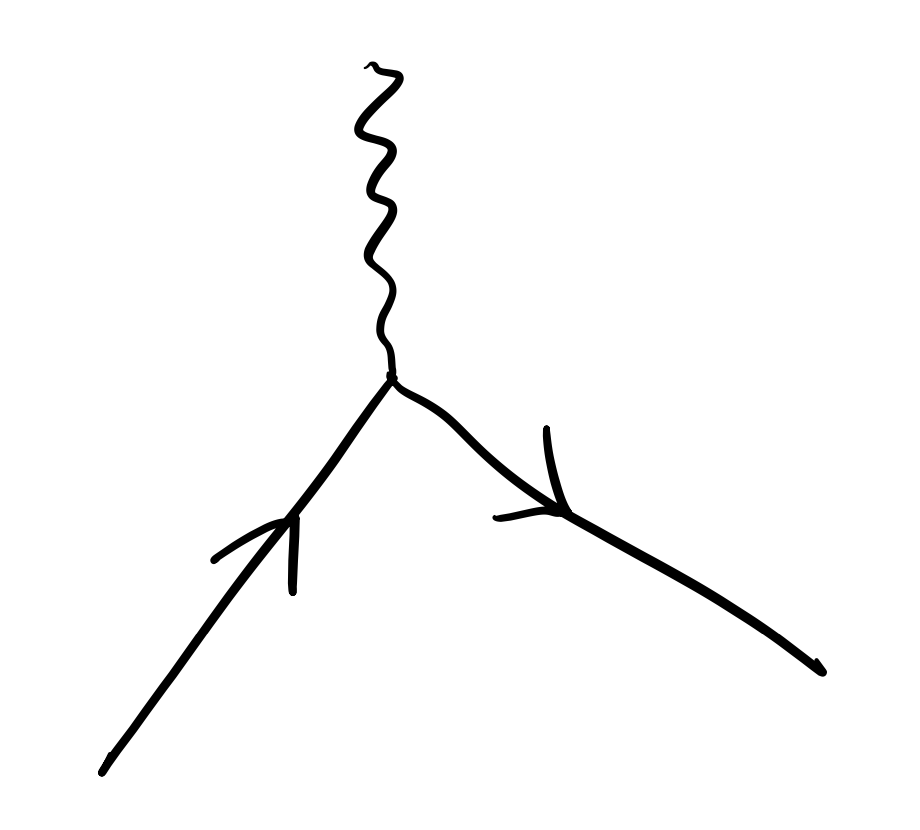
\includegraphics[scale=0.35]{Lectures/Images/lec9-diagram.png}
\end{center}

Let us first compute it in the free theory, using Wick contractions:
\begin{equation}
    \avg{j^\mu(x) \psi(y)\bar{\psi}(0)} = \avg{\bar{\psi}(x)\gamma^\mu \psi(x)\psi(y)\bar{\psi}(0)}
\end{equation}
The only connected correlators come from pairing $\psi(y)$ with $\bar{\psi}(x)$ (moving this fermion observable to pair them requires two moves, so no overall negative sign) and $\psi(x)$ with $\bar{\psi}(0)$ and thus we obtain:
\begin{equation}
    \avg{j^\mu(x) \psi(y)\bar{\psi}(0)} = G(y-x)\gamma^\mu G(x)
\end{equation}
Let us Fourier transform this (as this is where the Green's functions look simple):
\begin{equation}
    \avg{j^\mu_p \psi_{p'}\bar{\psi}} = \int d^4x d^4y e^{-ipx}e^{-ip'y}G(y - x)\gamma^\mu G(x) \stackrel{y \to z = y-x}{\to} \int_{zx} e^{-ipx}e^{-ip'(z + x)}G(z)\gamma^\mu G(x) = G(p')\gamma^\mu G(p + p')
\end{equation}
So in the free theory our vertex function looks like:

\begin{center}
    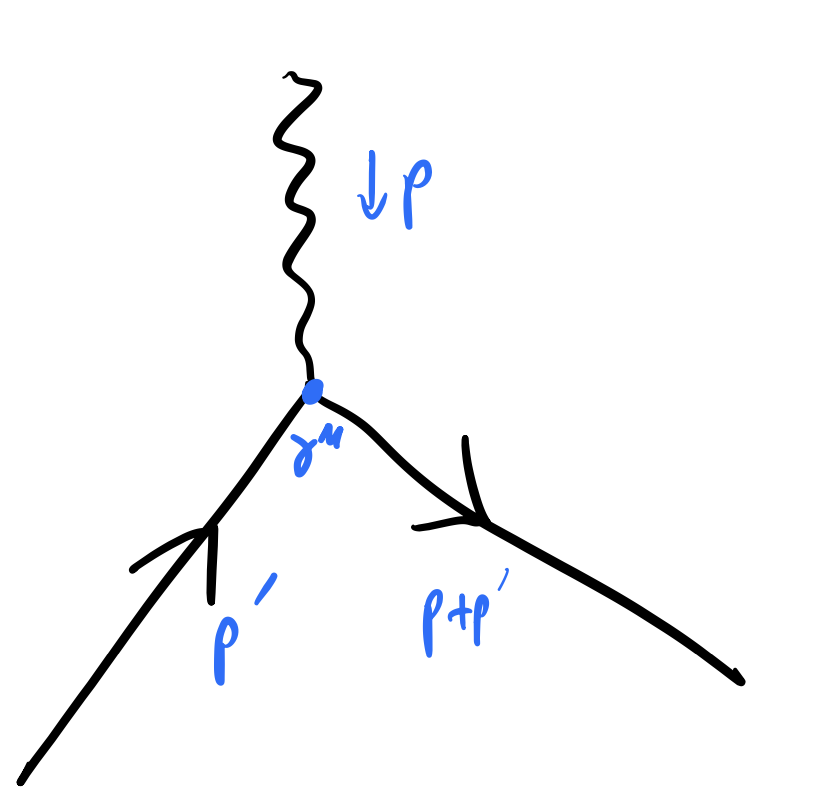
\includegraphics[scale=0.35]{Lectures/Images/lec9-free.png}
\end{center}

We can look at the ``amputated'' vertex, which will simply be obtained by multiplying the above by $G(p')^{-1} G(p+p')^{-1}$, which yields:
\begin{equation}
    \avg{j^\mu_p \psi_{p'}\bar{\psi}}_{\text{amp}} = \gamma^\mu
\end{equation}

So, we have the tree-level result. We are now interested in corrections to this answer. What kind of diagrams will give corrections to this vertex? At one loop we have three diagrams:

\begin{center}
    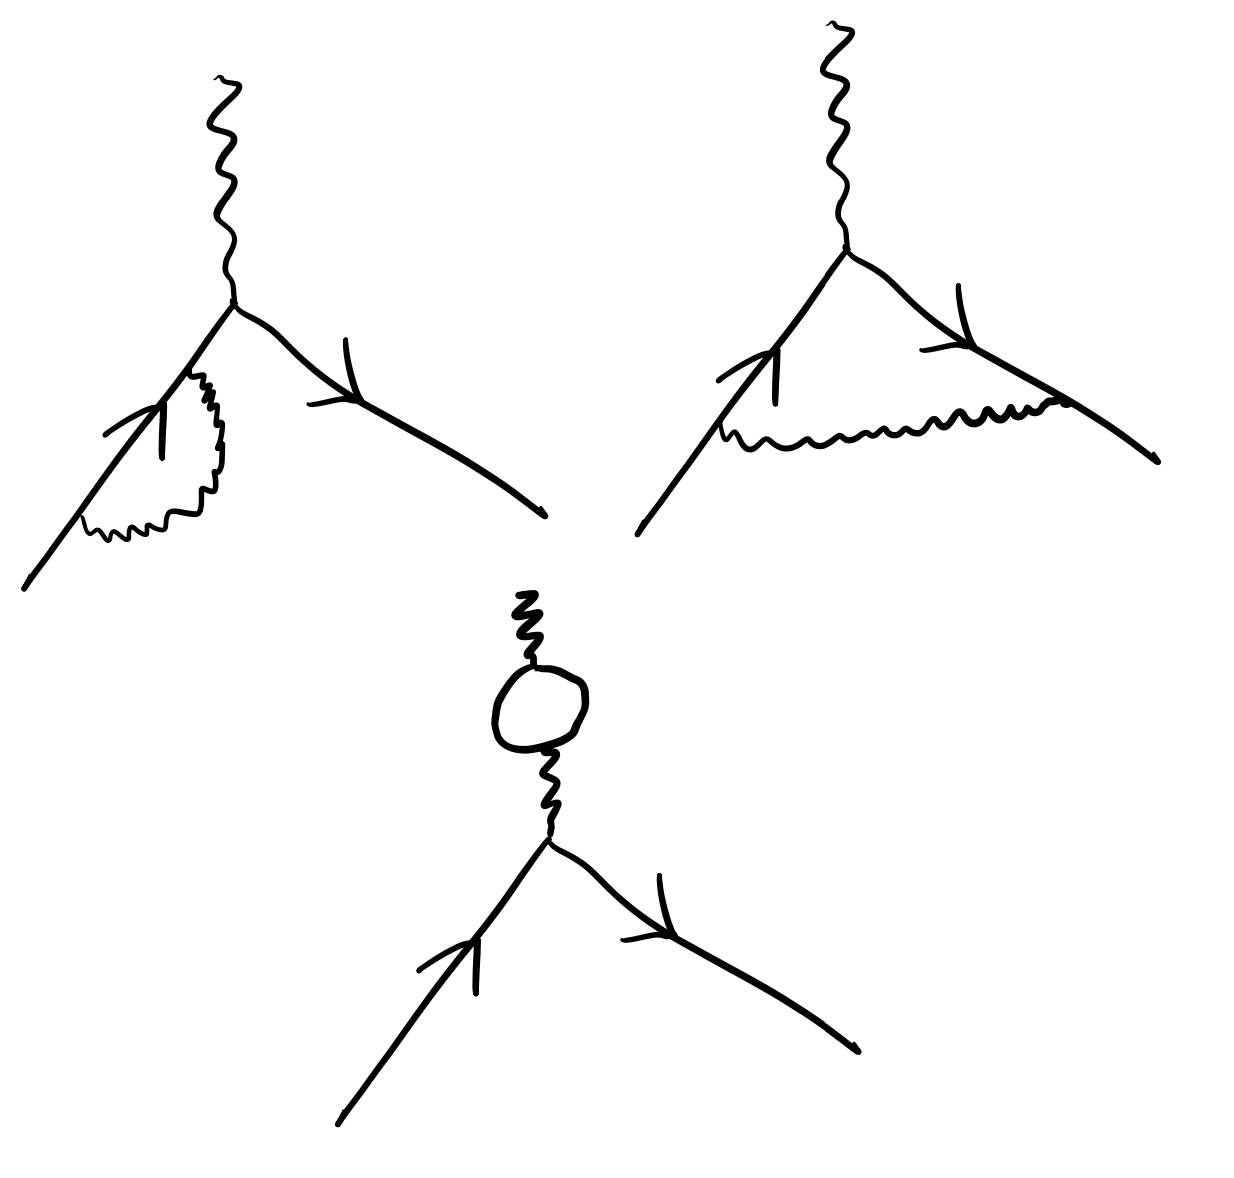
\includegraphics[scale=0.35]{Lectures/Images/lec9-oneloop.png}
\end{center}

In the interacting theory, the vertex function will take on a different form than the free theory. One can show that the most general form that it can take is:
\begin{equation}
    \avg{j^\mu_p \psi_{p'}\bar{\psi}}_{\text{amp}} = \gamma^\mu F_1(\frac{p^2}{m^2}) + iS^{\mu\nu}\frac{p_\nu}{m}F_2(\frac{p^2}{m^2}) 
\end{equation}
with:
\begin{equation}
    S^{\mu\nu} = \frac{i}{4}[\gamma^\mu, \gamma^\nu]
\end{equation}
In the free theory we had $F_1(\frac{p^2}{m^2}) = 1$ and $F_2(\frac{p^2}{m^2})  = 0$, but as we add corrections these functions will come alive. The $F_i$ are called ``form factors''. You can think about the above correlation function as probing the structure of the electron through:
\begin{equation}
    \avg{j^\mu_p\psi_{p'}\bar{\psi}} \sim \bra{p + p'}j^\mu \ket{p'}.
\end{equation}
Intuitively, the first term measures the renormalization of the charge $e$. The second term produces an ``anomalous'' electron dipole moment (which corrects for the classical prediction). How do we see this? One would get an $F_2$ contribution at tree level from a vertex:
\begin{equation}
    S_{\text{eff}} = \int \frac{a}{2m}F_{\mu\nu}\bar{\psi}S^{\mu\nu}\psi = -\int \frac{a}{m}\p_\nu A_\mu \bar{\psi}S^{\mu\nu}\psi
\end{equation}
with $\p_\nu A_\mu$ giving $ip_\nu$ and $a \sim F_2(0)$. Compare this with $A_\mu \bar{\psi}\gamma^\mu\psi$ which was our original vertex. Let's see how this term produces a dipole moment via studying the equation of motion:
\begin{equation}
    0 = \frac{\delta S}{\delta \bar{\psi}} = (i\slashed{D} - m + \frac{a}{2m}F_{\mu\nu}S^{\mu\nu})\psi
\end{equation} 
If we multiply this by the EOM with flipped sign:
\begin{equation}
    \begin{split}
        0 &= (i\slashed{D} + m - \frac{a}{2m}F_{\mu\nu}S^{\mu\nu})(i\slashed{D} - m + \frac{a}{2m}F_{\mu\nu}S^{\mu\nu})\psi 
        \\ &= (-\slashed{D}^2 - (m - \frac{a}{2m}F_{\mu\nu}S^{\mu\nu})^2)\psi
        \\ &\approx (-\slashed{D}^2 - m^2 + aF_{\mu\nu}S^{\mu\nu})\psi
        \\ &= (-D^2 - m^2 + (1 + a)F_{\mu\nu}S^{\mu\nu})\psi
    \end{split}
\end{equation}
Recall that $\slashed{D}^2 = D^2 - F_{\mu\nu}S^{\mu\nu}$, and this second term gave rise to the leading order electron dipole moment. So, the $a$ simply adds to this dipole moment, yielding:
\begin{equation}
    \mu = \frac{e}{2m}(1 + F_2(0))
\end{equation}
All of this to show that the new feature gives rise to the anomalous dipole moment.

Note that some qualities of the electron do not change via corrections (e.g. the number is protected) but others do (e.g. the dipole moment, for which we obtain small corrections in perturbation theory).

\subsection{Ward Identities for QED}
The vertex function is constrained by the Ward identity:
\begin{equation}
    \p_\mu \avg{j^\mu(x)\psi(y)\bar{\psi}(0)} = (\delta^4(x) - \delta^4(x-y))\avg{\psi(y)\bar{\psi}(0)}
\end{equation}
this is very useful as it relates the 4-point function to a 2-point function, and moreover, it holds non-perturbatively. Writing it in momentum space:
\begin{equation}
    -p_\mu \avg{j^\mu_p \psi_{p'}\bar{\psi}} = i[G(p') - G(p + p')]
\end{equation}
Thus, $p_\mu$ dotted with the four-point function just gives us the difference of two propagators (in the interacting theory, of course both sides of this equation become more complicated, but the identity still holds). Let's check this in the free theory as a consistency check. We consider the amputated versions here. On the LHS, we get $-\slashed{p}$, and on the RHS we have:
\begin{equation}
    \frac{1}{G(p')}i[G(p') - G(p + p')]\frac{1}{G(p+p')} = i\left(\frac{1}{G(p+p')} - \frac{1}{G(p')}\right) = i\left(\frac{\slashed{p} + \slashed{p}'}{-i} - \frac{\slashed{p}'}{-i}\right) = -\slashed{p}
\end{equation}
so the ward identity checks out.

\subsection{Proof of the form of the vertex function}
Let us call the fermion momenta $q_1$ and $q_2$. Using lorentz invariance we set $q_2 = -p - q_1$, and then we write down a general form:
\begin{equation}
    \avg{j^\mu_p \psi_{q_1}\bar{\psi}_{q_2}}_{\text{amp}} = q_1^\mu f_1 + q_2^\mu f_2 + f_3 \gamma^\mu f_4
\end{equation}
where the $f_i$ are matrices that depend only on lorentz covariant quantities:
\begin{equation}
    f_i(q_1^2, q_2^2, q_1\cdot q_2, \slashed{q}_1, \slashed{q}_2)
\end{equation}
This is a bit of a mess, it depends on too many parameters. To start, we put the fermions on shell $q_1^2 = q_2^2 = -m^2$. We will further sandwich it with spinors for which $(\slashed{p} + m)u(p) = 0$, these are precisely the spinors that we obtained when solving the Dirac equation, so sandwiching the above with $\bar{u}(q_1)\ldots u(q_2)$:
\begin{equation}
    \bar{u}(q_1)\avg{j^\mu_p \psi_{q_1}\bar{\psi}_{q_2}}u(q_2)
\end{equation}
this has a simple general form. Namely, we can move the $\slashed{q}_2$s to act them on the $u(q_2)$, giving $\slashed{q}_2u(q_2) = -mu(q_2)$ (and vise versa for $q_1$), which gives:
\begin{equation}
    \bar{u}(q_1)\avg{j^\mu_p \psi_{q_1}\bar{\psi}_{q_2}}u(q_2) = \bar{u}(q_1)(q_1^\mu f_1 + q_2^\mu f_2 + f_3\gamma^\mu)u(q_2)
\end{equation}
so we are down to three functions, and the $f_i$ are now just truly scalar functions rather than matrices, with $f_i = f_i(q_1 \cdot q_2)$. We are almost there, but we have three functions rather than the desired 2. Finally, we will use the fact that the vertex function must satisfy Ward identities, namely if we act on the above with $-p_\mu$ we get:
\begin{equation}
    \bar{u}(q_1)\left(\frac{1}{G(q_2)} - \frac{1}{G(q_1)}\right)u(q_2) = 0
\end{equation}
Which tells us that if we act on the vertex function with $p_\mu$ it must vanish, hence:
\begin{equation}
    0 = (p \cdot q_1 f_1 + p \cdot q_2 f_2)\bar{u}(q_1)u(q_2) + f_3\bar{u}(q_1)\slashed{p}u(q_2)
\end{equation}
The last term satisfies the Ward identity on its own; $\slashed{p} = -\slashed{q}_1 - \slashed{q}_2$, acting the two parts on the opposite sides, we find it vanishes:
\begin{equation}
    \bar{u}(q_1)(-\slashed{q}_1 - \slashed{q}_2)u(q_2) = \bar{u}(q_1)(-m + m)u(q_2) = 0
\end{equation}
Thus:
\begin{equation}
    0 = (q_1 + q_2)\cdot q_1f_1 + (q_1 + q_2)\cdot q_2 f_2 = (-2m^2+ 2q_1 \cdot q_2)(f_1 + f_2) \implies f_2 = -f_1
\end{equation}
where we have used $p^2 = (q_1 + q_2)^2 = -2m^2 + 2q_1 \cdot q_2$. And thus we only have two independent functions:
\begin{equation}
    \bar{u}(q_1)\avg{j^\mu_p \psi_{q_1}\bar{\psi}_{q_2}}u(q_2) = \bar{u}(q_1)\left(\gamma^\mu F_1(\frac{p^2}{m^2}) + (q_1^\mu - q_2^\mu)F_2(\frac{p^2}{m^2})\right)u(q_2)
\end{equation}
This is a very powerful statement because it is true non-perturbatively; it is always true!

On Thursday we continue the calculations by computing the corrections to the electron dipole moment at one loop.
\section{Radiative Corrections II}

\subsection{The Goal: One-Loop Correction to the Electron Dipole Moment}
Today we do the calculation to determine the correction to the electron dipole moment:
\begin{equation}
    \mu = \frac{e}{2m}(1 + \frac{\alpha}{2\pi} + O(\alpha^2))
\end{equation}
with:
\begin{equation}
    \frac{\alpha}{2\pi} = \frac{1}{2\pi}\frac{e^2}{2\pi} = \frac{1}{2\pi}\frac{e^2}{4\pi \e_0\hbar c} = 0.00116\ldots
\end{equation}
These are the promised 5 extra digits of precision that we obtain by going to one loop.

To find this, we will evaluate the correction to the vertex function:
\begin{equation}
    \delta \avg{j^\mu_p \psi \bar{\psi}_{p'}}_{\text{amp}} = \frac{1}{G(p + p')}\delta\avg{j^\mu_p \psi \bar{\psi}_{p'}} \frac{1}{G(p')}
\end{equation}
When the electron is on-shell, i.e. $p'^2 = -m^2 = (-\v{p} - \v{p}')^2$ and we sandwich the expression with $\bar{u}(\v{p} + \v{p}') \ldots u(\v{p}')$,  this has the general form:
\begin{equation}
    \delta \avg{j^\mu_p \psi \bar{\psi}_{p'}}_{\text{amp}} = \gamma^\mu F_1(\frac{p^2}{m^2}) + iS^{\mu\nu}\frac{p_\nu}{m}F_2(\frac{p^2}{m^2}) \stackrel{\text{free}}{\to} \gamma^\mu
\end{equation}
We will be particularly interested in:
\begin{equation}
    \mu = \frac{e}{2m}\left(1 + F_2(0)\right)
\end{equation}

\subsection{Which diagrams contribute?}
The diagram that produces $F_2$ is the one that is not a self-energy correction:
\begin{center}
    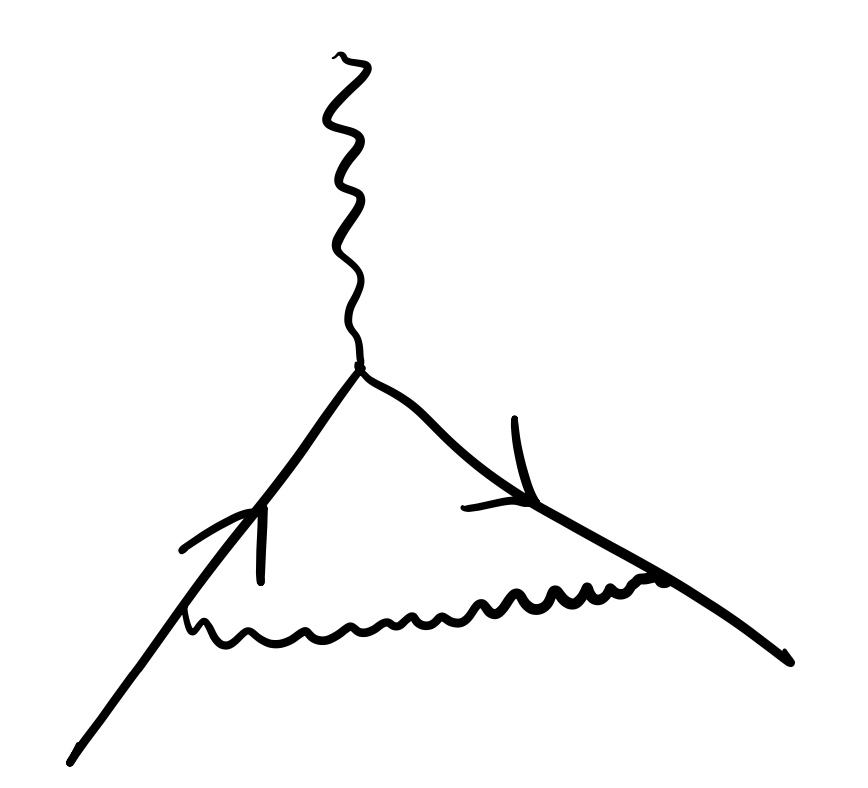
\includegraphics[scale=0.35]{Lectures/Images/lec10-relevantdiagram.png}
\end{center}

The self-energy correction to the dirac propagator only gives $\gamma^\mu$, as it renormalizes $G(p') = \slashed{p}'(\ldots) + \II(\ldots)$. The identity term gives the $\gamma^\mu$ and the first term (when sandwiching with the $u$s, which are solutions to the dirac equation and thus $(\slashed{q} + m)u(\v{q}) = 0 = \bar{u}(\v{q})(\slashed{q} + m)$) gives $-m$.
\begin{center}
    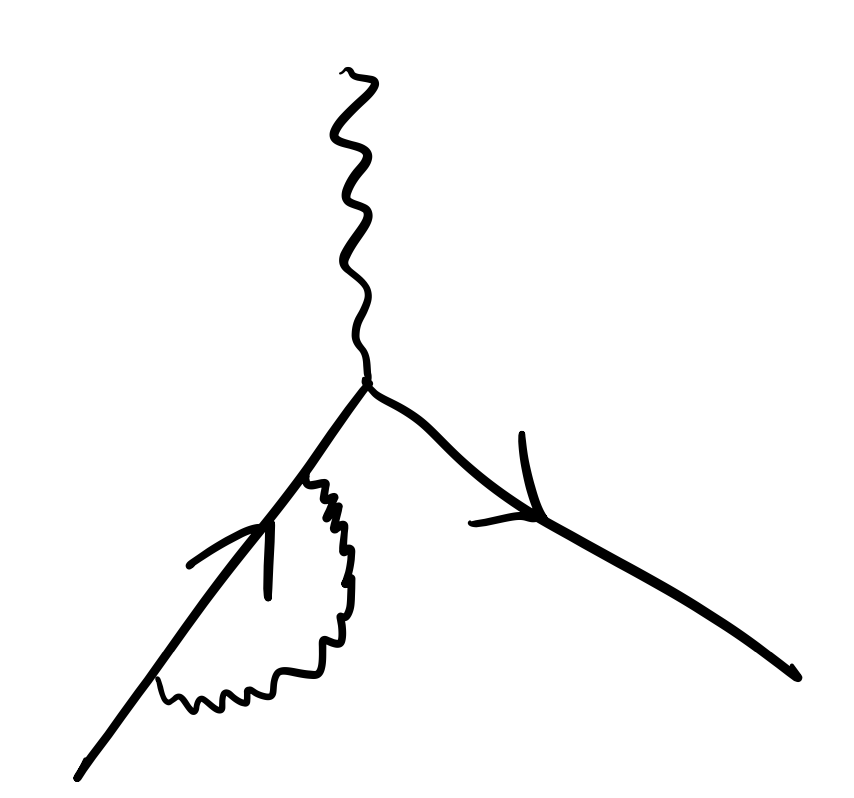
\includegraphics[scale=0.35]{Lectures/Images/lec10-diracselfE.png}
\end{center}
The self-energy correction to the photon also only gives $\gamma^\mu$. It renormalizes $G_{\mu\nu}(p) = \eta_{\mu\nu}(\ldots) + p_\mu p_\nu (\ldots)$, the $\eta_{\mu\nu}$ piece giving us $\gamma^\mu$, the $p_\mu p_\nu$ piece giving zero (why? $\bar{u}(\v{p} + \v{p}')\slashed{p})u(\v{p}') = 0$, because we can write $\slashed{p} = \slashed{p} + \slashed{p}' - \slashed{p}'$ and then acting on the left/right we get $\pm m$ which cancel. 
\begin{center}
    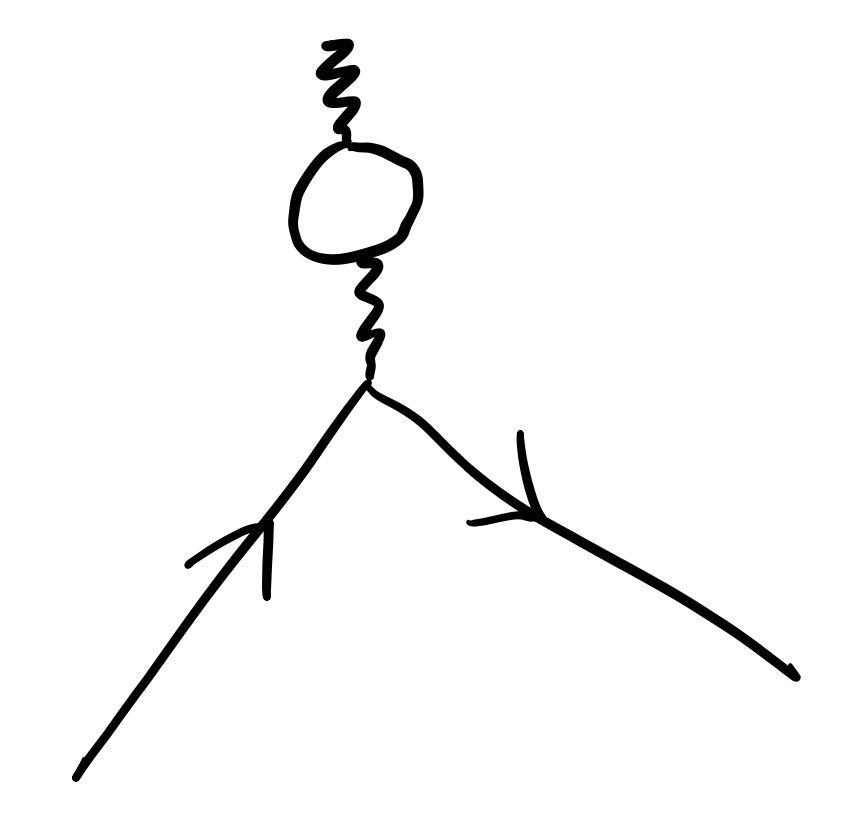
\includegraphics[scale=0.35]{Lectures/Images/lec10-photonselfE.png}
\end{center}
These diagrams will matter for other things - when we look at the renormalization and $\beta$ function of QED they are important (and you will look at the second diagram in the homework). But, for the $e^{-}$ dipole moment we only need consider the one diagram. Unfortunately, it is the most complicated, namely because we have a loop with three propagators. 

\subsection{Evaluating the 1-loop correction}
Graphically, the diagram (in momentum space) looks like:
\begin{center}
    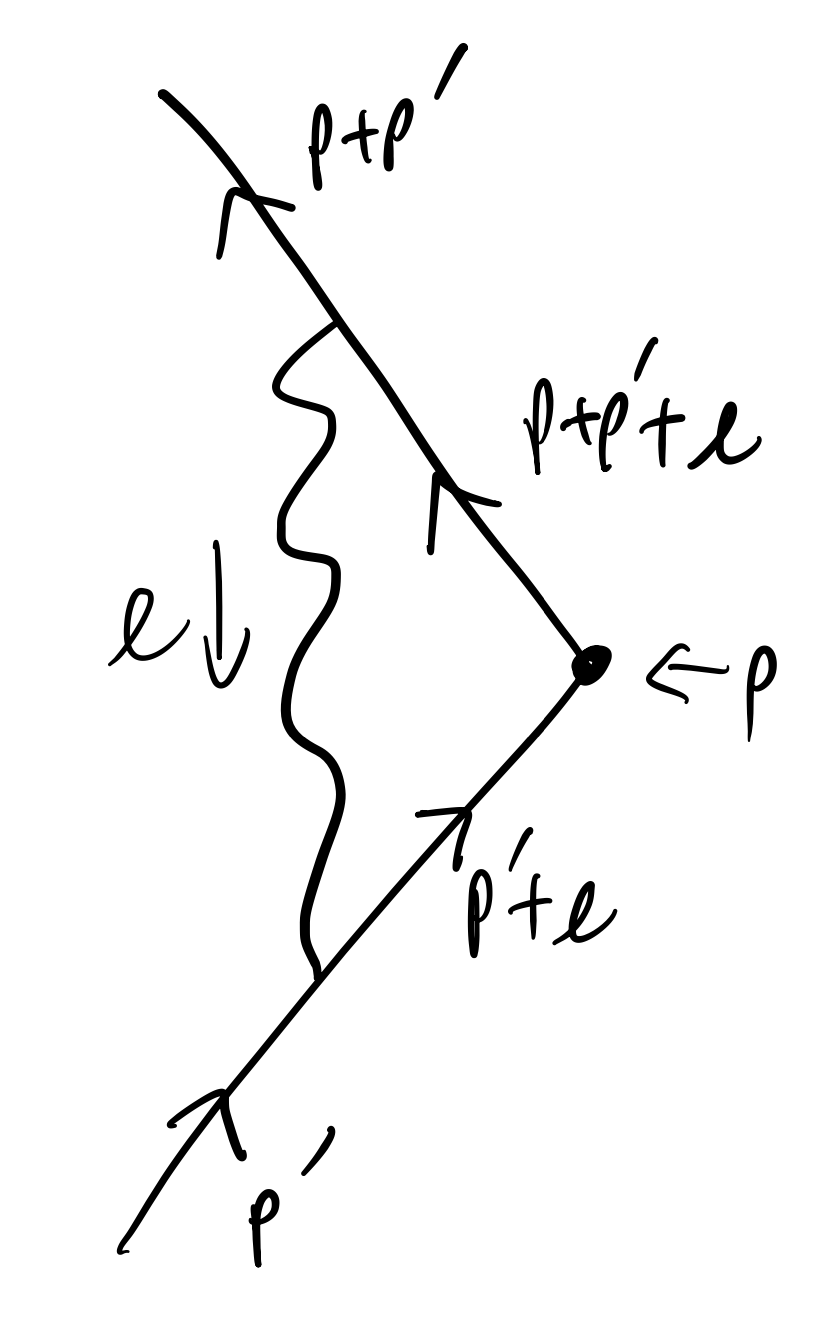
\includegraphics[scale=0.35]{Lectures/Images/lec10-momenta.png}
\end{center}

So our correction is of the form:
\begin{equation}
    \delta \avg{j^\mu_p \psi \bar{\psi}_{p'}} = \frac{i^2}{2}\avg{j^\mu_p \psi \bar{\psi}_{p'}(S_{\text{int}})^2} = -\frac{e^2}{2}\avg{(\bar{\psi}\gamma^\mu \psi)_p \left(\int_{x_1}A_\alpha \bar{\psi}\gamma^\alpha \psi \right)\left(\int_{x_2}A_\beta \bar{\psi}\gamma^\beta \psi \right)\psi \bar{\psi}_{p'}}
\end{equation}
We contract the $\psi$ in the current with $\bar{\psi}$ in the $x_1$ integral (2 possible choices, so factor of 2), and then $\bar{\psi}$ in the current with $\psi$ in the $x_2$ integral (we get a $-$ sign), then remaining $\bar{\psi}$ in $x_2$ with the $\psi$ on the right (another $-1$ sign) and $\psi$ in the $x_1$ with $\bar{\psi}$ on the right. When the smoke clears, we have:
\begin{equation}
    \delta \avg{j^\mu_p \psi \bar{\psi}_{p'}} = -e^2\int \frac{d^4l}{(2\pi)^4}G(p + p')\gamma^\beta G(p + p' + l)\gamma^\mu G(p' + l)\gamma^\alpha G(p') G_{\alpha\beta}(l)
\end{equation}
with the last term being the photon propagator (we have 4 dirac propagators and 1 photon propagator). We amputate this to make our lives simpler, which removes the $G(p + p')$ and $G(p')$:
\begin{equation}
    \delta \avg{j^\mu_p \psi \bar{\psi}_{p'}}_{\text{amp}} = -e^2\int \frac{d^4l}{(2\pi)^4}\gamma^\beta G(p + p' + l)\gamma^\mu G(p' + l)\gamma^\alpha G_{\alpha\beta}(l)
\end{equation}
Inserting our known expressions for the propagators (allowing ourselves to gauge fix with $\xi = 1$ such that we just have $G_{\alpha\beta}(l) = \frac{-i}{l^2}\eta_{\alpha\beta}$)
\begin{equation}
    \delta \avg{j^\mu_p \psi \bar{\psi}_{p'}}_{\text{amp}} = -e^2\int_l \gamma^\beta \frac{-i(\slashed{p} + \slashed{p}' + \slashed{l} - m)}{(p + p' + l)^2 + m^2}\gamma^\mu \frac{-i(\slashed{p}' + \slashed{l} - m)}{(p' + l)^2 + m^2}\gamma^\alpha \frac{-i}{l^2}\eta_{\alpha\beta}
\end{equation}
we will treat this in the usual way using Feynman parameters - with two propagators we used 1 Feynman parameter, with three propagators we shall use 2. We will use the identity (see Srednicki for the $n$-propagator version):
\begin{equation}
    \frac{1}{ABC} = 2\int_0^1 dx \int_0^{1-x}dy \frac{1}{[xA + yB + (1-x-y)C]^3}
\end{equation}
where we integrate over a triangle in the $xy$ plane. 
\begin{center}
    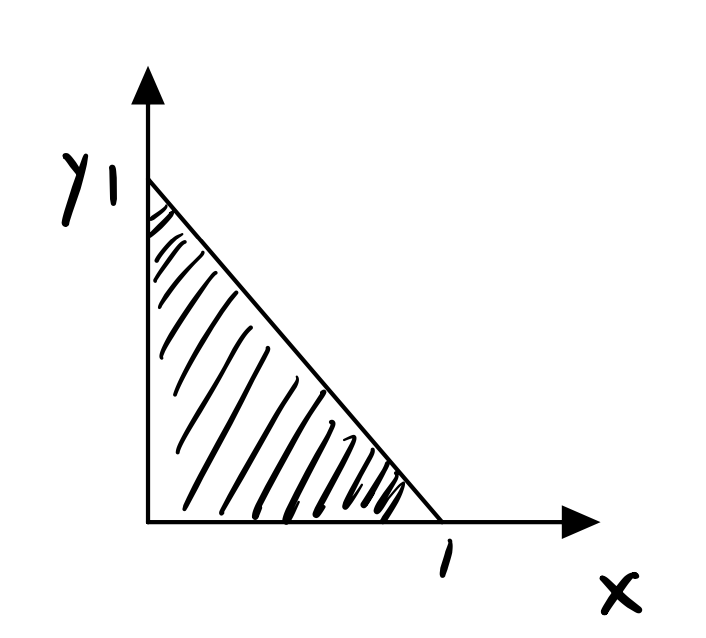
\includegraphics[scale=0.35]{Lectures/Images/lec10-triangle.png}
\end{center}
Applying this identity:
\begin{equation}
    \delta \avg{j^\mu_p \psi \bar{\psi}_{p'}}_{\text{amp}} = -2e^2\int_{xy}\int_l  \frac{-i(\slashed{p} + \slashed{p}' + \slashed{l} - m)\gamma^\mu \cdot -i(\slashed{p}' + \slashed{l} - m)\gamma^\alpha \cdot -i\eta_{\alpha\beta}}{l^2 + m^2(x+y) + p'^2x + (p + p')^2y + 2lp'x + 2l(p + p')y}
\end{equation}
Now writing the denominator as:
\begin{equation}
    \left([l + p'y + (p + p')x]^2 + m^2(x + y) + p'^2y + (p + p')^2x - [p'y + (p+p')x]^2\right)^3
\end{equation}
Renaming $[l + p'y + (p + p')x] = q$ and $\Delta(x, y) = m^2(x + y) + p'^2y + (p + p')^2x - [p'y + (p+p')x]^2$, we have:
\begin{equation}
    \delta \avg{j^\mu_p \psi \bar{\psi}_{p'}}_{\text{amp}} = -2ie^2\int_q \int_{xy}\frac{\gamma^\alpha((1-x)(\slashed{p} + \slashed{p}') - y\slashed{p}' + \slashed{q} -m)\gamma^\mu((1-y)\slashed{p}' - x(\slashed{p}+\slashed{p}') + \slashed{q} - m)\gamma_\alpha}{[q^2 + \Delta]^3}
\end{equation}
we have made the numerator terrible at expense of making the denominator simple, but the odd-in-q parts will integrate to zero via parity symmetry.

\subsection{UV divergent part}
Does this integral have a UV divergence? Indeed, it goes as $\sim \int d^4q \frac{q^2}{q^6}$ which is a logarithmic divergence. In more detail, the UV divergent part looks like:
\begin{equation}
    \delta \avg{j^\mu_p \psi \bar{\psi}_{p'}}_{\text{amp}} = -2ie^2\int_{xy}\int_q\frac{\gamma^\alpha \slashed{q}\gamma^\mu \slashed{q}\gamma_\alpha}{[q^2 + \Delta]^3}
\end{equation}
and now using the identity:
\begin{equation}
    \gamma^\alpha \slashed{p}\slashed{k}\slashed{q}\gamma_\alpha = 2\slashed{q}\slashed{k}\slashed{p}
\end{equation}
we have (taking the derivative w.r.t. $k_\mu$) and the case where $p = q$:
\begin{equation}
    \gamma^\alpha \slashed{q}\gamma^\mu \slashed{q}\gamma_\alpha = 2\slashed{q}\gamma^\mu \slashed{q} = 2\slashed{q}(-\slashed{q}\gamma^\mu - 2q^\mu) = 2q^2\gamma^\mu - 4\slashed{q}q^\mu
\end{equation}
Thus:
\begin{equation}
    \delta \avg{j^\mu_p \psi \bar{\psi}_{p'}}_{\text{amp}} = -4ie^2\int_{xy}\int_q\frac{q^2\gamma^\mu - 2q^\mu q^\nu \gamma_\nu}{[q^2 + \Delta]^3} = -4ie^2\gamma_\nu \int_{xy}\int_q\frac{q^2\eta^{\mu\nu} - 2q^\mu q^\nu}{[q^2 + \Delta]^3}
\end{equation}
Since the integral is isotropic, we can replace the second term:
\begin{equation}
    q^\mu q^\nu = \eta^{\mu\nu}q^2\frac{1}{4}
\end{equation}
and so:
\begin{equation}
    \delta \avg{j^\mu_p \psi \bar{\psi}_{p'}}_{\text{amp}} = -2ie^2\gamma_\mu \int_{xy}\in_{q}\frac{q^2}{[q^2 + \Delta]^3}
\end{equation}
so, we notice that the entire UV divergent term is $\propto \gamma^\mu$ and as such does not enter the correction to the electron dipole moment. It will be relevant for renormalizing the electron charge. But, let's still compute this because we will still care about this when we study RG for QED. We recover the $-i\e$ in the denominator:
\begin{equation}
    \delta \avg{j^\mu_p \psi \bar{\psi}_{p'}}_{\text{amp}} = -2ie^2\gamma_\mu \int_{xy}\in_{q}\frac{q^2}{[q^2 + \Delta-i\e]^3}
\end{equation}
which shifts the poles of $q_0$ off the real axis, and we can choose an appropriate contour (see below)
\begin{center}
    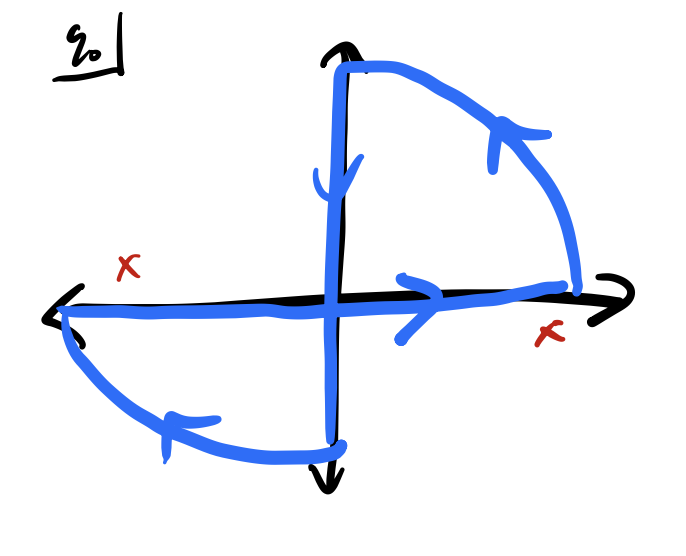
\includegraphics[scale=0.35]{Lectures/Images/lec10-contour.png}
\end{center}
which gives us the Wick rotation $q_0 \to iq_0^E$, allowing us to compute the (real) integral:
\begin{equation}
    \delta \avg{j^\mu_p \psi \bar{\psi}_{p'}}_{\text{amp}} = 2e^2\gamma^\mu \int_{xy}\int_{q_E}\frac{q^2}{[q^2 + \Delta]^3} = 2e^2\gamma^\mu \int_{xy}\frac{2\pi^2}{(2\pi)^4}\int_0^\infty dq \frac{q^5}{[q^2 + \Delta]^3} = \frac{e^2\gamma^\mu}{4\pi^2}
\end{equation}
In Wilsonian RG, we integrate $b\Lambda < q < \Lambda$ with $\Lambda \gg m, p, p', \Delta^{1/2}$, so we obtain:
\begin{equation}
    \delta \avg{j^\mu_p \psi \bar{\psi}_{p'}}_{\text{amp}} = -\frac{e^2\gamma^\mu}{4\pi^2}\int_{xy}\int_{b\Lambda}^\Lambda \frac{dq}{q} = \frac{e^2}{8\pi^2}\log(\frac{1}{b})\gamma^\mu
\end{equation}
where he $xy$ integral is now trivial and gives 1/2. This thus gives the renormalization of charge:
\begin{equation}
    \gamma^\mu(1 + \frac{e^2}{8\pi}\log(\frac{1}{b}))
\end{equation}
note there are other diagrams that contribute here, which we will need when we do RG. We did this with a cutoff here, but it is not a good idea to do here as it breaks gauge invariance. In the HW you will look at dimensional regularization. The $\log(\frac{1}{b})$ gets replaced with $-\frac{1}{\e}$ where $\e$ is the regulated dimension.

\subsection{Back to the electron dipole moment}
So, we found that the $O(q^2)$ term only matters when we do RG and not for the dipole moment. Further, the $O(q)$ terms go to 0 by $q \leftrightarrow -q$ symmetry. So, we can just set $q = 0$ and see what remains; after Wick rotation:
\begin{equation}
    \delta \avg{j^\mu_p \psi \bar{\psi}_{p'}}_{\text{amp}} = 2e^2\int_{xy}\int_q \frac{\gamma^\alpha((1-x)(\slashed{p} + \slashed{p}') - y\slashed{p}' - m)\gamma^\mu(\slashed{p}'(1-y) - x(\slashed{p} + \slashed{p}') - m)\gamma_\alpha}{[q^2 + \Delta]^3}
\end{equation}
Now the $q$-integral is easy because only the denominator has $q$ dependence:
\begin{equation}
    \int_q \frac{1}{[q^2 + \Delta]^3} = \frac{2\pi^2}{(2\pi)^4}\int_0^\infty \frac{dq q^3}{[q^2 + \Delta]^3} = \frac{1}{8\pi^2}\frac{1}{\Delta}\int_0^\infty \frac{ds s^3}{(s^2 + 1)^3} = \frac{1}{32\pi^2}\frac{1}{\Delta}
\end{equation}
So then:
\begin{equation}
    \delta \avg{j^\mu_p \psi \bar{\psi}_{p'}}_{\text{amp}} = \frac{e^2}{16\pi^2}\int_{xy}\frac{1}{\Delta}(\gamma^\alpha((1-x)(\slashed{p} + \slashed{p}') - y\slashed{p}' - m)\gamma^\mu(\slashed{p}'(1-y) - x(\slashed{p} + \slashed{p}') - m)\gamma_\alpha)
\end{equation}
Let's look at the numerator. We showed that it has to take the form:
\begin{equation}
    \bar{u}(\v{p}+ \v{p}') \ldots u(\v{p}') =  \bar{u}(\v{p}+ \v{p}')\gamma^\mu F_1(\frac{p^2}{m^2}) + iS^{\mu\nu}\frac{p_\nu}{m}F_2(\frac{p^2}{m^2})u(\v{p}')
\end{equation}
So, lets take this numerator and simplify this when we sandwich it via $u$s. Let's invoke the $\gamma$ matrix technology:
\begin{equation}
    \gamma^\alpha \slashed{p}\slashed{q}\gamma_\alpha = 4p\cdot q
\end{equation}
\begin{equation}
    \gamma^\alpha \slashed{p}\gamma_\alpha = 2\slashed{p}
\end{equation}
so then with $a = (1-x)(p + p') - yp'$, $b = (1-y)p' - y(p + p')$.
\begin{equation}\label{eq:lec10temp}
    \gamma^\alpha (\slashed{a} - m)\gamma^\mu (\slashed{b} - m)\gamma_\alpha = 2\slashed{b}\gamma^\mu \slashed{a} - 4(a^\mu + b^\mu)m + 2m^2\gamma^\mu
\end{equation}
we can drop the $\gamma^\mu$ terms (again these do not contribute to the $F_2$ term). Now using the EOM of the spinors:
\begin{equation}
    (\slashed{p}' + m)u(\v{p}') = 0 = \bar{u}(\v{p} + \v{p}')(\slashed{p} + \slashed{p}' + m)
\end{equation}
The first term of Eq. \eqref{eq:lec10temp} becomes:
\begin{equation}
    \begin{split}
        2\slashed{b}\gamma^\mu \slashed{a} &= 2((1-y)\slashed{p}' + xm)\gamma^\mu ((1 - x)(\slashed{p} + \slashed{p}') + ym) 
        \\ &= 2xy m^2\gamma^\mu + 2y(1-y)\slashed{p}\gamma^\mu + 2\gamma^\mu  (\slashed{p} + \slashed{p}')x(1-x)m + 2(1-y)(1-x)\slashed{p}'\gamma^\mu (\slashed{p} + \slashed{p}')
    \end{split}
\end{equation}
We can drop the $\propto \gamma^\mu$ term. Using more Dirac algebra, we can write this as:
\begin{equation}
    2\slashed{b}\gamma^\mu \slashed{a} = (\text{number}) \gamma^\mu - 4im(1-x-y)(x + y)S^{\mu\nu}p_\nu
\end{equation}
So our final integral is:
\begin{equation}
    \delta \avg{j^\mu_p \psi \bar{\psi}_{p'}}_{\text{amp}} = \frac{ie^2m}{4\pi^2}S^{\mu\nu}p_\nu \int_{xy}\frac{(1-x-y)(x+y)}{\Delta(x, y, p, p')}
\end{equation}
We are interested in the low energy limit where $\v{p} \to 0$ so $p'^2 \to -m^2$, $(p + p')^2 = -m^2$ (finite $\v{p}$ would tell you about the shape beyond the dipole) then $\Delta = m^2(x^2 + y^2)$ and so:
\begin{equation}
    \delta \avg{j^\mu_p \psi \bar{\psi}_{p'}}_{\text{amp}} \approx \frac{ie^2}{4\pi^2}\frac{S^{\mu\nu}p_\nu}{m}\int_{xy}\frac{(1-x-y)}{x+y} = \frac{ie^2}{8\pi^2}\frac{S^{\mu\nu}p_\nu}{m} = \frac{e^2}{8\pi^2}\frac{iS^{\mu\nu}p_\nu}{m}
\end{equation}
So we find:
\begin{equation}
    F_2(0) = \frac{e^2}{8\pi^2} = \frac{1}{2\pi}\alpha
\end{equation}
and so:
\begin{equation}
    \boxed{\mu = \frac{e}{2m}\left(1 + \frac{\alpha}{2\pi} + \ldots\right)}
\end{equation}
which is what we set out to show!
\section{QED $\beta$-function}
QED is an interacting quantum field theory, which has a dimensionless coupling between the photons and fermions. This means that interesting things can happen. Classically, the effect seems marginal, but we know that these statements do not survive quantum corrections. So, we study how these couplings flow under the renormalization group, which tells us the regime in which perturbation theory is valid.

Recall the QED path integral in the $R_\xi$ gauge:
\begin{equation}
    Z = \int \mathcal{D}A\mathcal{D}\psi \exp(i\int \bar{\psi}(i\slashed{D} - m)\psi - \frac{1}{4}F^2 - \frac{1}{2\xi}(\p_\mu A^\mu)) = \int \mathcal{D}A\mathcal{D}\psi e^{iS_0 + iS_{\text{int}}}
\end{equation}
with:
\begin{equation}
    D_\mu = \p_\mu + iA_\mu.
\end{equation}
The only non-Gaussian (and hence interaction) term in the action is:
\begin{equation}
    S_{\text{int}} = -e\int A_\mu \bar{\psi}\gamma^\mu \psi
\end{equation}

\subsection{Review of the Renormalization Group}
Last quarter, we saw how to do renormalization in the Wilsonian style, where we assume that some modes above some momentum $\Lambda$ have been already integrated out (removing any UV divergences), and then we perform an additional step of integrating out modes $b\Lambda < p < \Lambda$ (with $0 < 1 - b \ll 1$) and see how the couplings evolve under the process. This will tell us whether terms in the action will become more important or not.

\begin{center}
    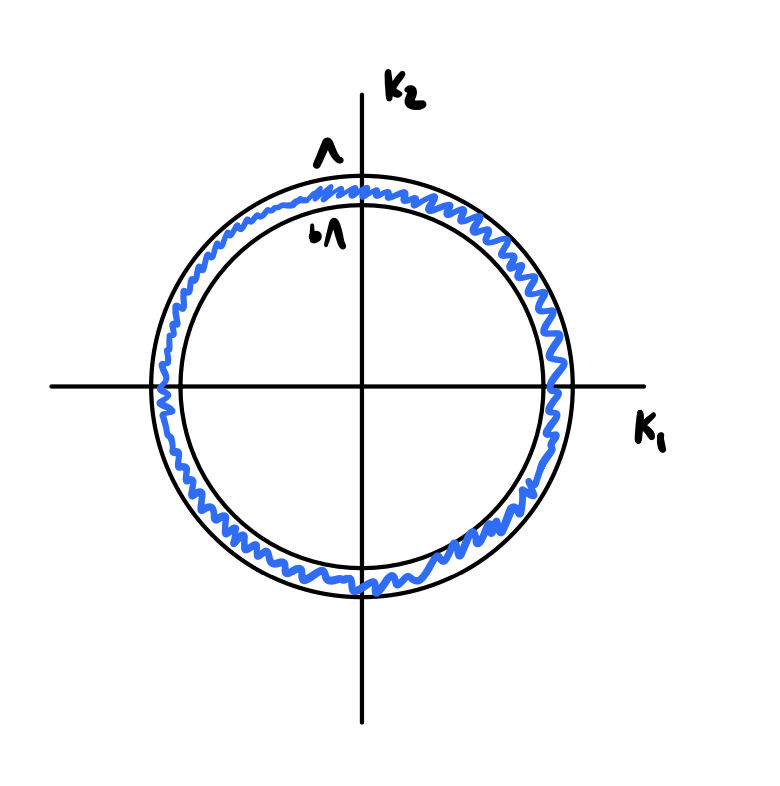
\includegraphics[scale=0.35]{Lectures/Images/lec11-energyshell.png}
\end{center}

Recall that in the scalar field case, we had:
\begin{equation}
    \phi(x) = \int_{p < \Lambda}e^{-ipx}\phi_p = \int_{p < b\Lambda}e^{-ipx}\phi_p + \int_{b\Lambda < p < \Lambda}e^{ipx}\phi_p = \phi_{b\Lambda} + \tilde{\phi}
\end{equation}
We then consider splitting the functional integral:
\begin{equation}
    \begin{split}
        Z &= \int \mathcal{D}\phi_\Lambda e^{iS[\phi]} 
        \\ &= \int \mathcal{D}\phi_{b\Lambda} e^{iS_0[\phi]}\int \mathcal{D}\tilde{\phi}e^{iS_0[\tilde{\phi}]}e^{iS_{\text{int}}[\phi, \tilde{\phi}]}
        \\ &= \int \mathcal{D}\phi_{b\Lambda} e^{iS_0[\phi]}\left(e^{i\delta S_{\text{eff}}[\phi]}\right)
        \\ &= \int \mathcal{D}\phi_{b\Lambda}e^{iS_{\text{eff}}[\phi]}
    \end{split}
\end{equation}
In the final step, we rescale coordinates such that:
\begin{equation}
    S_{\text{eff}} = \int d^4x \ldots = \int d^4\tilde{x} \ldots
\end{equation}
where:
\begin{equation}
    \tilde{x} = xb \implies \tilde{p} = \frac{p}{b} < \Lambda
\end{equation}
and canonically normalize.

\subsection{Applying RG to QED}
Before this final step, we expect the effective QED action will look like:
\begin{equation}
    S_{\text{eff}} = \int_x (1 + \delta_2)\bar{\psi}i\slashed{\p}\psi - (m + \delta m)\bar{\psi}\psi - (1 + \delta_1)eA_\mu \bar{\psi}\gamma^\mu \psi - \frac{1 + \delta_3}F^2 + \ldots
\end{equation}
where the $\ldots$ denotes irrelevant terms. We now rescale $x = \tilde{x}/b$ (and drop the $\tilde{}$s):
\begin{equation}
    S_{\text{eff}} = \int_x \frac{Z_2}{b^3}\bar{\psi}i\slashed{\p}\psi - \frac{m + \delta m}{b^4}\psi\bar{\psi} - \frac{Z_1e}{b^4}A_\mu \bar{\psi}\gamma^\mu \psi -\frac{Z_3}{4b^2}F^2 + \ldots
\end{equation}
We then canonically normalize:
\begin{equation}
    \psi \to \frac{b^{3/2}}{\sqrt{Z_2}}\psi, \quad A \to \frac{b}{\sqrt{Z_3}}A
\end{equation}
in order to normalize the kinetic terms. We then obtain:
\begin{equation}
    S_{\text{eff}} = \int_x \bar{\psi} i\slashed{\p}\psi  - \frac{m + \delta m}{bZ_2}\bar{\psi}\psi - \frac{Z_1 e}{Z_2\sqrt{Z_3}}A_\mu \bar{\psi}\gamma^\mu \psi - \frac{1}{4}F^2 + \ldots
\end{equation}
so we then have the new mass and coupling:
\begin{equation}
    \begin{split}
        m(b) &= \frac{m + \delta m}{bZ_2}
        \\ e(b) &= \frac{Z_1e}{Z_2\sqrt{Z_3}}
    \end{split}
\end{equation}
We can thus obtain the scale dependence of the couplings. Starting with $m$, which already has scale dependence at tree level ($Z \to 1, \delta m \to 0$):
\begin{equation}
    \beta_m \equiv \dod{m(b)}{\log b} = b\dod{m(b)}{b} = -m(b) < 0
\end{equation}
so $m$ is relevant (this was already clear from dimensional analysis). At lower and lower energies, mass matters more and more. The much more interesting thing to figure out is the scale dependence of $e$ - we already knew it was dimensionless from dimensional analysis, and this manifests in the $e(b)$ expression where there are no explicit factors of $b$ present. At tree level, $\beta_e = 0$ (marginal). Beyond tree level:
\begin{equation}
    \beta_e = \dod{}{\log b}\left(\frac{Z_1}{Z_2\sqrt{Z_3}}\right)e = e\dod{}{\log b}\frac{1 + \delta_1}{(1 + \delta_2)(1 + \delta_3)^{1/2}} \approx e\dod{}{\log b}\left(1 + \delta_1 - \delta_2 - \frac{1}{2}\delta_3\right)
\end{equation}

\subsection{Dimensional Regularization}
It is possible to study this with sharp cutoffs, but this breaks gauge invariance. So, it's not the best choice. A more convenient regulator in QED is is dimensional regularization - because dimension enters analytically in all of our formulas and loop integrals, we can analytically continue into $d = 4 - \e$. As you saw in your homework, $\log\Lambda$ divergences that come from dimensionless couplings with sharp cutoffs get replaced by $\frac{1}{\e}$ divergences ($\e \to 0$ to get back to 4 dimensions, so $\e^{-1}$ holds the UV divergences). More precisely, in RG, something like $\int \frac{d^4p}{p^4}$ becomes (with a sharp cutoff):
\begin{equation}
    \int_{b\Lambda}^\Lambda \frac{dp}{p} = \log\frac{\Lambda}{b\Lambda} = \log\frac{1}{b}
\end{equation}
vs. with dimensional regularization:
\begin{equation}
    \int_0^\infty \frac{dp}{p}p^{-\e} = \left.-\frac{1}{\e}p^{-\e}\right|_\mu^\infty = \frac{1}{\e}\mu^{-\e} = \frac{1}{\e}e^{-\e\log \mu} \approx \frac{1}{\e}(1 - \e\log\mu + \ldots) = \frac{1}{\e} - \log \mu
\end{equation}
so in the RG setting $\log\frac{1}{b}$s get replaced with $\frac{1}{\e}$s. As an example, we perform the following Feynman integral via the sharp cutoff method:
\begin{equation}
    \int_{b\Lambda}^\Lambda \frac{pdp}{p^2 + \Delta} = \left.\frac{1}{2}\log(p^2 + \Delta)\right|_{b\Lambda}^\Lambda = \frac{1}{2}\log\frac{\Lambda^2 + \Delta}{(b\Lambda)^2 + \Delta} \approx \log(\frac{1}{b}) + C\log\Delta + \ldots
\end{equation}
and via the dim reg method:
\begin{equation}
    \int_0^\infty \frac{p^{1-\e}dp}{p^2 + \Delta} = \frac{\pi}{2}\frac{1}{\sin(\frac{\e\pi}{2})}\Delta^{-\frac{\e}{2}} \approx \frac{1}{\e + O(\e^3)}\left(1 - \frac{\e}{2}\log\Delta + \ldots\right) = \frac{1}{\e} - \frac{1}{2}\log \Delta + \ldots
\end{equation}
The dim reg method provides the same results, but does allow us to compute things without breaking gauge invariance.

\subsection{Renormalizing the QED Coupling}
We start by computing $Z_3$, which corresponds to the renormalization of the photon propagator. You already did this in your homework, and we will see that $Z_1 = Z_2$ via a Ward identity, so this actually is the most important part. The diagram of interest is the one loop ($\avg{j^\mu j^\nu}$) diagram:

\begin{center}
    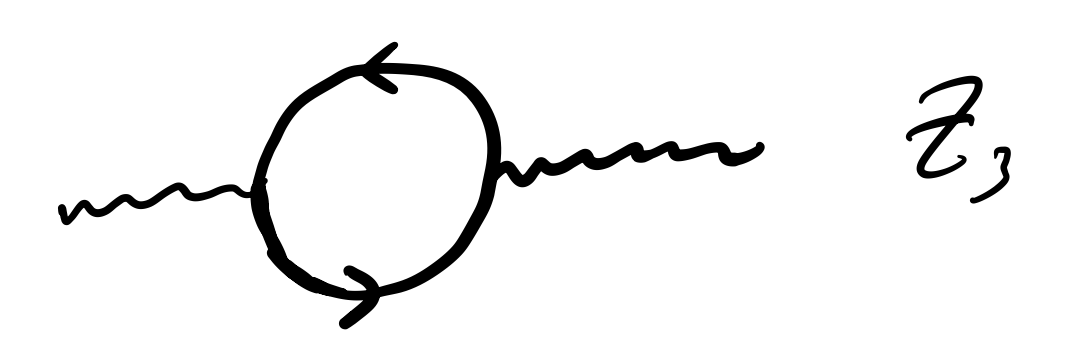
\includegraphics[scale=0.35]{Lectures/Images/lec11-Z3.png}
\end{center}

We have:
\begin{equation}
    S_{\text{int}}[\tilde{\phi}, \phi] \supset -e A_\mu \tilde{\bar{\psi}}\gamma^\mu \tilde{\psi}
\end{equation}
as the fermions get integrated out, so:
\begin{equation}
    Z = \int \mathcal{D}\phi e^{iS_0[\phi]}\int \mathcal{D}\tilde{\phi}e^{iS_{\text{int}}[\phi, \tilde{\phi}]}e^{iS_0[\tilde{\phi}]}
\end{equation}
expanding out the interacting action as a power series, the first contributing term is:
\begin{equation}
    \frac{i^2}{2}S_{\text{int}}^2 = -\frac{e^2}{2}\int_{x_1}A_\mu \tilde{\bar{\psi}}\gamma^\mu \tilde{\psi}\int_{x_2}A_\nu \tilde{\bar{\psi}}\gamma^\nu \tilde{\psi}
\end{equation}
So:
\begin{equation}
    \begin{split}
        \int \mathcal{D}\tilde{\phi}\frac{i^2}{2}S_{\text{int}}^2e^{iS_0[\tilde{\phi}]} &= -\frac{1}{2}e^2\int_1\int_2 A_\mu(x_1)A_\nu(x_2)\avg{j^\mu(x_1)j^\nu(x_2)}
        \\ &= -\frac{e^2}{2}\int \frac{d^4p}{(2\pi)^4}A_\mu(p)A_\nu(-p)\avg{j^\mu j^\nu}(p)
        \\ &= i\delta S_{\text{eff}}[\psi, A]
    \end{split}
\end{equation}
In your homework, you found that the current two point function was:
\begin{equation}
    \avg{j^\mu j^\nu}(p) = (p^2\eta^{\mu\nu} - p^\mu p^\nu)\frac{i}{6\pi^2}\frac{1}{\e}
\end{equation}
Therefore:
\begin{equation}
    S_{\text{eff}} = -\frac{e^2}{6\pi^2}\frac{1}{\e}\frac{1}{2}\int\frac{d^4p}{(2\pi)^4}A_\mu(-p)A_\nu(p)(p^2\eta^{\mu\nu} - p^\mu p^\nu)
\end{equation}
This looks identical to the Maxwell term:
\begin{equation}
    S_0 \supset -\frac{1}{2}\int_p A^\mu_p A^\nu_p(p^2 \eta^{\mu\nu} - p^\mu p^\nu)
\end{equation}
which is perhaps not surprising; we have a gauge invariant regulator, so we should get a gauge invariant result. We could have generated other gauge invariant terms, but these would contain higher derivatives; we focus on the terms that have a chance of being relevant. From this, we can identify the renormalization term $Z_3$:
\begin{equation}
    S_{\text{eff}} -\frac{1}{4}\left(1 + \frac{e^2}{6\pi^2}\frac{1}{\e}\right)\int_x F^2
\end{equation}
\begin{equation}
    Z_3 = 1 + \frac{e^2}{6\pi^2}\frac{1}{\e} \to 1 - \frac{e^2}{6\pi^2}\log(b)
\end{equation}
So we have the key ingredient in:
\begin{equation}
    \beta_e = \dod{}{\log b}\frac{Z_1}{Z_2\sqrt{Z_3}}e.
\end{equation}
We still need to calculate $Z_1, Z_2$. 

\begin{center}
    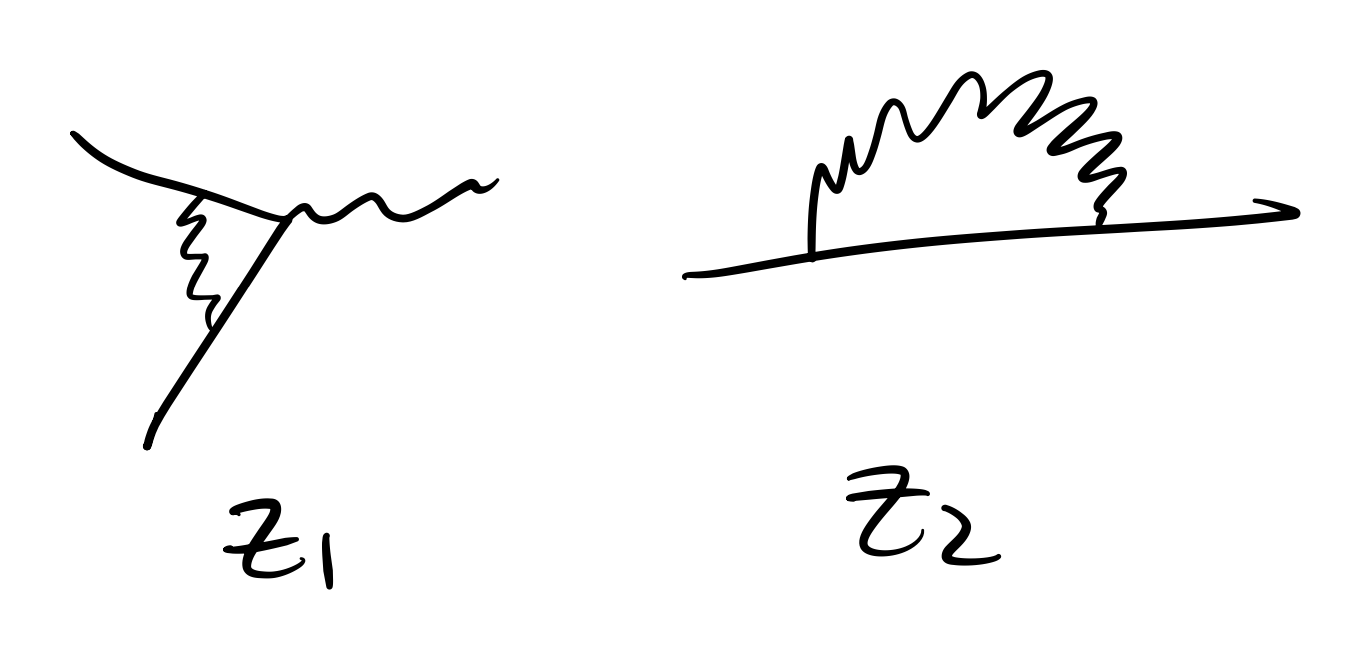
\includegraphics[scale=0.35]{Lectures/Images/lec11-Z1Z2.png}
\end{center}

But the ward identity implies they are equal (this will be the last thing we do this lecture). Thus the ratio drops out, and we end up with:
\begin{equation}
    \beta_e = \dod{}{\log b}\frac{e}{\sqrt{Z_3}} = e\dod{}{\log b}(1 - \frac{1}{2}\delta_3) = -\frac{e}{2}\dod{\delta_3}{\log b} = \frac{e^3}{12\pi^2} > 0
\end{equation}
Thus! $\beta_e > 0$ and so the coupling is \emph{irrelevant} under RG. Therefore, the interactions shrink at lower and lower energies. This also makes sense that it was one of the first QFTs to be discovered; we have access to low energies, and this is a regime where perturbation theory is controlled.

Conversely, interactions grow at higher energies, which tells us that QED is \emph{not} UV complete. In nature, this is UV-completed by the theory of non-abelian gauge fields.

\subsection{Last Step - Ward Identity}
We go through the argument of the Ward identity implying $Z_1 = Z_2$. We had shown that a consequence of the Ward identity was:
\begin{equation}
    i\p_\mu \avg{j^\mu_p \psi \bar{\psi}_{p'}} = G(p') - G(p+p')
\end{equation}
and in the amputated case:
\begin{equation}
    i\p_\mu \avg{j^\mu_p \psi \bar{\psi}_{p'}}_{\text{amp}} = \frac{1}{G(p + p')} - \frac{1}{G(p')}
\end{equation}
Where in the free theory:
\begin{equation}
    ip_\mu \gamma^\mu = i\slashed{p} \stackrel{?}{=} \frac{\slashed{p} + \slashed{p}' + m}{-i} - \frac{\slashed{p}' + m}{-i} = i\slashed{p}
\end{equation}
In the interacting theory, the vertex gets renormalized,so the LHS becomes:
\begin{equation}
    \gamma^\mu Z_1 = \avg{j^\mu \psi\bar{\psi}}_{\text{amp}}
\end{equation}
and the fermion propagator gets normalized:
\begin{equation}
    S_{\text{eff}} \supset \int Z_2\bar{\psi}i\slashed{\p}\psi \implies G(p) = \frac{-i}{Z_2\slashed{p} + (m + \delta m)}
\end{equation}
so the RHS becomes:
\begin{equation}
    Z_2i\slashed{p}
\end{equation}
This implies:
\begin{equation}
    i\slashed{p} Z_2 = i\slashed{p}Z_2 \implies Z_1 = Z_2.
\end{equation}
This is not at all obvious from looking at the Feynman diagrams leading to these two terms; they look different and the 1-loop calculations are tedious. Such is the power of symmetry!

Thus, we've deduced the fate of QED. Next, we will slightly switch gears, and study scattering in QED (where the setting is richer, e.g. due to particles having spin). Further, there is a subtlety when looking at scattering of massless particles - the existence of a mass gap was crucial for well-separating the single-particle excitations from the two-particle continuum. We don't have this in QED due to the photons being gapless. So the S-matrix of QED does not formally exist. So what have people been doing for the last century? It is possible to work out these subtleties, which we will go through. The fundamental problem is we can't distinguish whether we have a particle or $n$ super low energy photons. Naively we get IR divergences (large wavelength phenomena) which gets out of control. We'll see how to control it, next.
\section{Scattering in QED}
\subsection{LSZ for Fermions}
Today we move to the last big topic in QFT II! We'll derive the LSZ formula for Dirac fermion and photons. We will go back to our Hamiltonian expressions to derive it, and then after deriving, compute the S-matrix amplitudes via path integrals.

We recall the solutions to the Dirac equation found via mode expansion:
\begin{equation}
    \psi(x) = \sum_{s=\pm}\int \frac{d^3p}{(2\pi)^32\e_{\v{p}}}[b_{s, \v{p}}u_s(\v{p})e^{ipx} + d^\dag_{s, \v{p}}v_s(\v{p})e^{-ipx}]
\end{equation}
with:
\begin{equation}
    u_s(\v{0}) = \sqrt{m}\m{1\\0\\1\\0}, \quad
\end{equation}
and:
\begin{equation}
    \set{b_{s\v{p}}, b_{s'\v{p}'}} = 2\e_{\v{p}}(2\pi)^3\delta^3(\v{p} - \v{p}')\delta_{ss'}
\end{equation}
We also inverted these equations to get $b/d$ in terms of the quantum field $\psi$:
\begin{equation}\label{eq:bdagddag}
    \begin{split}
        b^\dag_{s, \v{p}} &= \int d^3xe^{ipx}\bar{\psi}(x)\gamma^0 u_s(\v{p})
        \\ d^\dag_{s, \v{p}} &= \int d^3x e^{ipx}\bar{v}_s(\v{p})\gamma^0 \psi(x)
    \end{split}
\end{equation}
Note the time dependence present in the exponential (with $p^0 = \e_p = \sqrt{\v{p}^2 + m^2}$) gets cancelled with the time dependent part of $\psi$ to make the overall expressions time-independent.

In the free theory, these operators are time-independent, and these operators create single-particle states:
\begin{equation}
    \begin{split}
        b^\dag_{s, \v{p}} &= \ket{\v{p}, s, e}
        \\ d^\dag_{s, \v{p}} &= \ket{\v{p}, s, -e}
    \end{split}
\end{equation}
In the free theory, these states are boring - the states are time-independent and nothing happens to them. In the interacting theory, we would like to build scattering states. The $b^\dag_{s, \v{p}}(t)$ and $d^\dag_{s, \v{p}}(t)$ defined via Eq. \eqref{eq:bdagddag} will have time-dependence in the interacting theory (because we don't know how $e^{iHt}$ acts in the interacting theory). Put another way:
\begin{equation}
    b^\dag_{s, \v{p}}(t) \ket{0} \neq b^\dag_{s, \v{p}}(t') \ket{0}
\end{equation}
for $t \neq t'$. We want to construct single-particle states for early and late times. The intuition is that at a specific time, $b^\dag_{s, \v{p}}(t) \ket{0}$ ``looks'' like a single-particle state, even though it may time evolve nontrivially.

So - our states that are simple at asymptotically early times (the ``in'-states here for two fermions) are:
\begin{equation}
    \ket{i} = b^\dag_{s_1, \v{p}_1}(-\infty)b^\dag_{s_2, \v{p}_2}(-\infty)\ket{0}
\end{equation}
And the states that are simple at late times (the ``out''-states) are:
\begin{equation}
    \ket{f} = b^\dag_{s_3, \v{p}_3}(\infty)b^\dag_{s_4, \v{p}_4}(\infty)\ket{0}
\end{equation}
The reason this works is that even though we have not identified the true multi-particle states, our guess has some overlap with the true multi-particle states.
\begin{equation}
    \bra{\v{p}, s, e}b^\dag_{s, \v{p}}\ket{0} \neq 0
\end{equation}
so we may appropriately normalize and use our ansatz as the in/out states. The intuition is that well-separated wavepackets are non-interacting.

We also require that overlap with multiparticle states vanishes:
\begin{equation}
    \bra{\v{p}, s, \v{p}', s'}b^\dag_{s, \v{p}}(-\infty)\ket{0} = 0
\end{equation}
this crucially hinges on the existence of a finite mass gap between the single particle states and the multi-particle continuum. Indeed this will cause trouble in QED, as though the electrons have mass, the photons are massless.

\begin{center}
    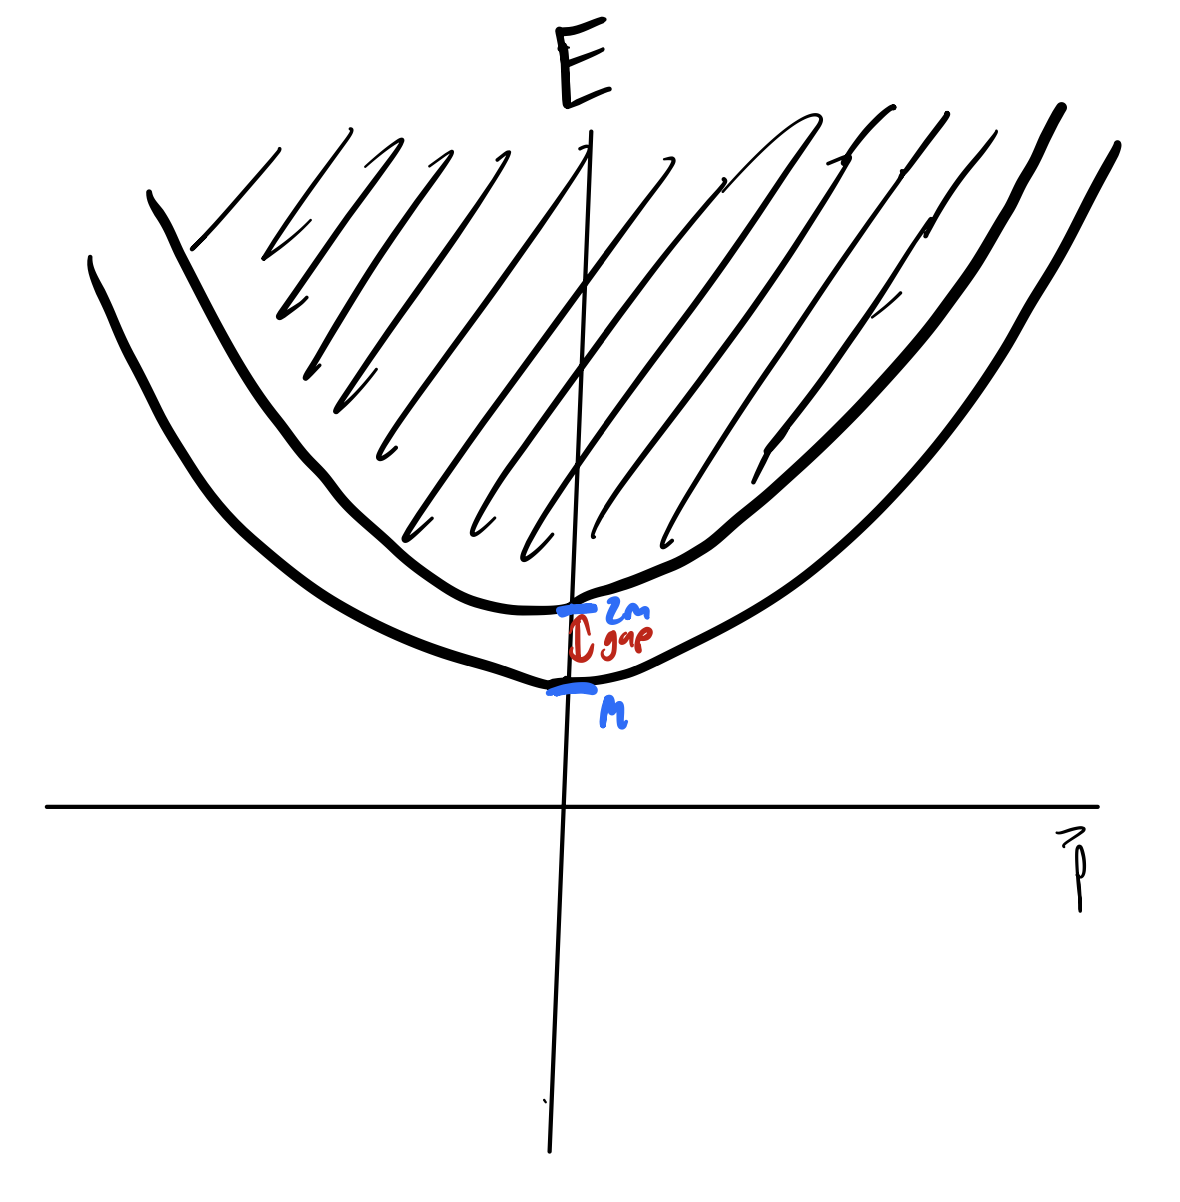
\includegraphics[scale=0.35]{Lectures/Images/lec12-massgap.png}
\end{center}

So, let's find a formula for the probability that a given in state goes to a given out state, $p(i\to f)$, given by the (square of) the matrix elements $S_{fi} = \bra{f}{i}$. As for the scalar field, we work out the difference between two creation operators:
\begin{equation}
    \begin{split}
        b^\dag_{s, \v{p}}(\infty) - b^\dag_{s, \v{p}}(-\infty) &= \int_{-\infty}^\infty dt \p_t b_{s, p}
        \\ &= \int d^4x \p_t(e^{ipx}\bar{\psi}(x)\gamma^0u_s(\v{p}))
        \\ &= \int d^4x e^{ipx}(ip_0 + \p_0)\bar{\psi}(x)\gamma^0u_s(\v{p})
    \end{split}
\end{equation}
the above equation reminds us of $(\slashed{p} + m)u_s(\v{p}) = 0$, so then:
\begin{equation}
    b^\dag_{s, \v{p}}(\infty) - b^\dag_{s, \v{p}}(-\infty) = \int d^4x\bar{\psi}(\overleftarrow{\p_0} \gamma^0 - ip_i \gamma^i - im)u_s(\v{p})e^{ipx}
\end{equation}
If we now integrate by parts (in space); we can replace $ip_i = \overrightarrow{\p_i}$ with $-\overleftarrow{\p_i}$ and so:
\begin{equation}
    \begin{split}
        b^\dag_{s, \v{p}}(\infty) - b^\dag_{s, \v{p}}(-\infty) &= \int d^4x \bar{\psi}(\overleftarrow{\slashed{p}} - im)u_s(\v{p})e^{ipx}
        \\ &= -i\int d^4x \bar{\psi}(i\overleftarrow{\slashed{p}} + m)u_s(\v{p})e^{ipx}
    \end{split}
\end{equation}
Taking the conjugate of this expression, we similarly find:
\begin{equation}
    b_{s, \v{p}}(\infty) - b_{s, \v{p}}(-\infty) = i\int d^4x e^{-ipx}\bar{u}_s(\v{p})(-i\slashed{\p} + m)\psi
\end{equation}
So now we did the same thing we did for our scalar field theory. We plug these expressions into the expression for the $S$-matrix elements:
\begin{equation}
    \braket{f}{i} = \bra{0}\mathcal{T}b_{s_3, \v{p}_3}(\infty)b_{s_4, \v{p}_4}(\infty)b^\dag_{s_1, \v{p}_1}(-\infty)b^\dag_{s_2, \v{p}_2}(-\infty)\ket{0}
\end{equation}
where we have introduced a time-ordering operator for free - we can now replace the $b^\dag, b$s with the differences that we computed above, which are equivalent due to the time ordering (time ordering kills the other terms by virtue of $b\ket{0} = \bra{0}b^\dag = 0$ - the mass gap assumption guarantees that the annihilation operators still annihilate the vacuum of the theory). We are left with:
\begin{equation}
    \begin{split}
        \braket{f}{i} = i^4\int_{x_1x_2x_3x_4}&e^{-ip_3x_3 - ip_4x_4}[\bar{u}_{s_3p_3}(-i\slashed{\p}_{x_3} + m)]_{\alpha}[\bar{u}_{s_4p_4}(-i\slashed{p}_{x_4} + m)]_{\beta}\bra{0}\mathcal{T}\psi_{\alpha}(x_3)\psi_{\beta}(x_4)\bar{\psi}_{\gamma}(x_1)\bar{\psi}_{\delta}(x_2)\ket{0}
        \\ &\cdot [(i\overleftarrow{\slashed{\p}}_{x_1} + m)u_{s_1}(\v{p}_1)]_\gamma[(i\overleftarrow{\slashed{\p}}_{x_2} + m)u_{s_2}(\v{p}_2)]_\delta e^{ip_1x_1 + ip_2x_2}
    \end{split}
\end{equation}
This looks complicated, but the extra factors actually end up being useful - they amputate the external propagators and put the particle on-shell. This condition drastically reduces the dependencies on the variables - for the scalar case we reduced things to Mandelstam variables $s, t, u$ (only of which 2 were independent), and although things are more complicated here due to the presence of spin indices, again things will simplify.

\begin{center}
    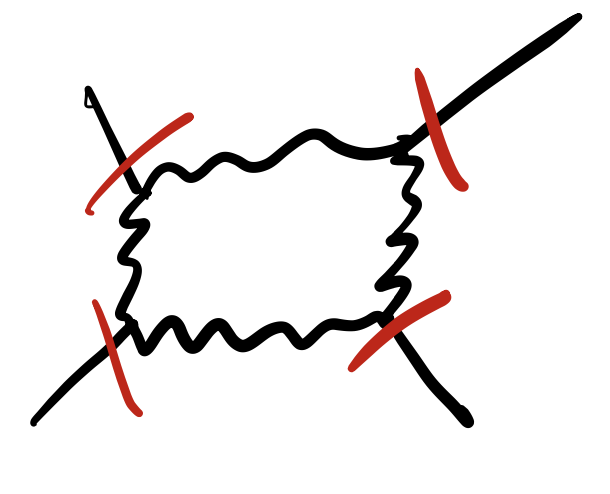
\includegraphics[scale=0.35]{Lectures/Images/lec12-amputatedlegs.png}
\end{center}

The expression actually looks much simpler in momentum space. Like for scalars $\braket{f}{i} = \delta_{if} + T_{if}$, we can use momentum conservation to write:
\begin{equation}
    iT_{if} = (2\pi)^4\delta^4(p_1 + p_2 - p_3 - p_4)i\mathcal{M}(p_1p_2 \to p_3p_4)
\end{equation}
which leaves us with:
\begin{equation}
    \begin{split}
        &i\mathcal{M}(p_1p_2 \to p_3p_4) = 
        \\ &[\bar{u}_{s_3}(\v{p}_3)(\slashed{p}_3 + m)]_\alpha [\bar{u}_{s_4}(\v{p}_4)(\slashed{p}_4 + m)]_\beta \avg{\mathcal{T}\psi_{\alpha}(\v{p}_3)\psi_{\beta}(\v{p}_4)\bar{\psi}_\gamma(\v{p}_1)\bar{\psi}_\gamma}_c [(\slashed{p}_1 + m)u_{s_1}(\v{p_1})]_\gamma[(\slashed{p}_2 + m)u_{s_2}(\v{p_2})]_\delta
    \end{split}
\end{equation}
where we see that the expressions in brackets $[\cdot]$ are just the inverse propagators, which amputate the external legs.

\subsection{LSZ for photons}
We saw that photons have two propagating degrees of freedom, which we labelled with helicity $\pm 1$. We expect naively:
\begin{equation}
    \braket{\ldots}{\v{p}, h} = \e^h_\mu (p^2\eta^{\mu\nu} + (\xi - 1)p^\mu p^\nu)\avg{\mathcal{T}A_\nu\ldots}
\end{equation}
Naively, it looks like we could choose 4 polarizations, $\e_\mu = \delta_\mu^0, \delta^x_\mu, \delta^y_\mu, \delta^z_\mu$. We will see that due to Gauge invariance, only two polarizations are physical.

Let's set $p^\mu = (p, 0, 0, p)$, with $p^z = p^0$, and $(p^\mu)^2 = 0$ as required. Helicity is an eigenvalue under $J_3$ with this choice. Now consider $\e^{(x)}_\mu = \delta^x_\mu$ and $\e^{(y)}_\mu = \delta^y_\mu$. These vectors get exchanged under $J_2$ rotation:
\begin{equation}
    \m{\e^{(x)} \\ \e^{(y)}} \to \m{\cos\theta & \sin\theta \\ -\sin\theta & \cos\theta}\m{\e^{(x)} \\ \e^{(y)}}
\end{equation}
So we have the eigenvectors $\e^\mp_\mu = \e^{(x)}_\mu \mp i\e^{(y)}_\mu$; to see this:
\begin{equation}
    \e^{(x)}_\mu \mp i\e^{(y)}_\mu \mapsto \cos\theta \e^{(x)} + \sin\theta \e^{(y)} \mp i(\cos\theta \e^{(y)}  - \sin\theta \e^{(x)}) = (\cos\theta \pm i\sin\theta)(\e^{(x)} \mp i\e^{(y)}) = e^{\pm i\theta}\e^{\mp}
\end{equation}
These are the states we expect to be physical. They have an important property that they are orthogonal to the wavevector:
\begin{equation}
    \e^{\pm}_\mu p^\mu = 0
\end{equation}
which tells us that this is gauge invariant. One way to be orthogonal to $p^\mu$ is to take $p_\mu$, but $\e^\pm_\mu$ are \emph{not} the null vector; they are vectors orthogonal in the Minkowski metric that are orthogonal to momentum without being the momentum itself.

Our guess for the LSZ formula thus simplifies (as the gauge dependent part gets killed):
\begin{equation}
    \braket{\ldots}{\v{p}, h} = \e^h_\mu p^2\avg{\mathcal{T}A^\mu\ldots}
\end{equation}
What happens to the other polarizations? They do produce physical states, but correspond to the pure gauge component $A_\mu \sim \p_\mu \lambda$ and the constrained variable.
\begin{equation}
    \e^\mu_1 = (1, 0, 0, 1) \propto p^\mu
\end{equation}
\begin{equation}
    \e^\mu_2 = (1, 0, 0, -1)
\end{equation}
$\e^\mu_1$ vanishes, since it gives $p^\mu p^2\avg{A_\mu \ldots }$ which vanishes via the Ward identity. $\e^\mu_2$ probes the pure gauge piece, since $\e^\mu_2(\xi - 1)p_\mu p_\nu \neq 0$, and hence is not gauge invariant (and hence unphysical).

\begin{center}
    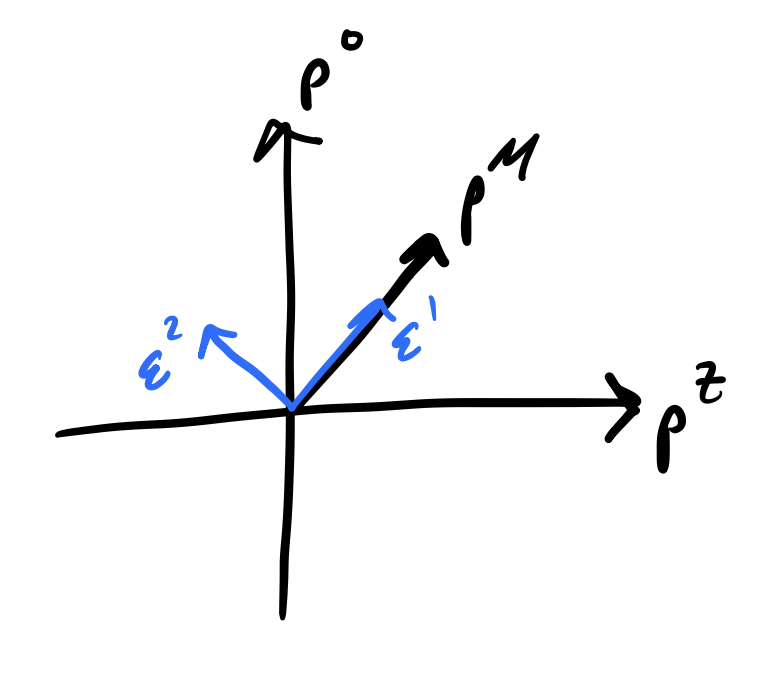
\includegraphics[scale=0.35]{Lectures/Images/lec12-unphysicalpolarizations.png}
\end{center}


So, the LSZ formula for $\gamma\gamma \to \gamma\gamma$ scattering is:
\begin{equation}
    \braket{f}{i} = i^4\int_{x_1x_2x_3x_4}e^{i(p_1x_2 + p_2x_2 - p_3x_3 - p_4x_4)}(\p_{x_1}^2\p_{x_2}^2\p_{x_3}^2\p_{x_4}^2)\e^{\mu_1}_{h_1}\e^{\mu_2}_{h_2}\e^{\mu_3}_{h_3}\e^{\mu_4}_{h_4}\avg{\mathcal{T}A_{\mu_1}(x_1)A_{\mu_2}(x_2)A_{\mu_3}(x_3)A_{\mu_4}(x_4)}
\end{equation}
Again this has a cleaner form when we Fourier transform:
\begin{equation}
    i\mathcal{M} = p_1^2p_2^2p_3^2p_4^2\e^{\mu_1}_{h_1}\e^{\mu_2}_{h_2}\e^{\mu_3}_{h_3}\e^{\mu_4}_{h_4}\avg{0}\mathcal{T}A_{\mu_1}(p_1)A_{\mu_2}(p_2)A_{\mu_3}(p_3)A_{\mu_4}(p_4)\ket{0}_c
\end{equation}
Much like in the scalar and fermion case, we have that the external legs are amputated.

\subsection{Do Photons Scatter?}
The simplest diagram that contributes to $\mathcal{M}$ looks like:

\begin{center}
    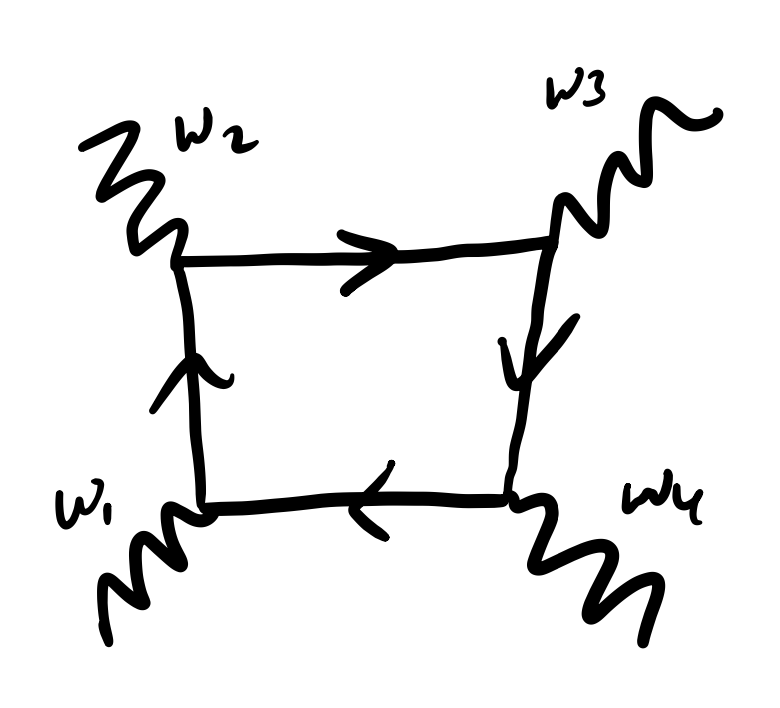
\includegraphics[scale=0.35]{Lectures/Images/lec12-photonscatterdiagram.png}
\end{center}


QED tells us that the superposition principle is incorrect; we have nonlinear effects that cause photons to scatter. But, this diagram is very small, so the superposition principle is approximately correct. Let's estimate how small this is. We have:
\begin{equation}
    \frac{m_ec^2}{\hbar} \sim 10^{21}\si{Hz}
\end{equation}
while visible light has:
\begin{equation}
    \omega \sim 10^{14}\si{Hz}
\end{equation}
the diagram goes as $\sim \frac{\omega^4}{m_e^4}\alpha^2 \sim 10^{-32}$.

In deriving the photon LSZ formula, we made a leap of faith, postulating the form of it assuming that there was a mass gap. But of course there is not. The approach we will take is to ignore it until we cannot ignore it - things will eventually go wrong. At tree level, scattering in QED looks fine. But once we start studying loops, things will not make sense. When we have loops, we have higher powers of the coupling, so we start including terms with more external photons, wherein we will have to return to this problem.
\section{Scattering in QED II}
Recall the LSZ formula we found for $e^-e^-\to e^-e^-$
\begin{equation}
    i\mathcal{M}(p_1p_2\to p_3p_4) = i^4[\bar{u}_4(\slashed{p}_4 + m)]_\delta [\bar{u}_3(\slashed{p}_3 + m)]_\gamma \avg{\mathcal{T}\psi_\delta(p_4)\psi_\gamma(p_3)\bar{\psi}_\beta(p_2)\bar{\psi}_\alpha(p_1)}_C[(\slashed{p}_2 + m)u_2]_\beta[(\slashed{p}_1 + m)u_1]_\alpha
\end{equation}
One can similarly show that for $e^+e^+ \to e^+e^+$ (you will show this on the pset - though we can guess the solution. $\psi \sim b + d^\dag$, so):
\begin{equation}
    i\mathcal{M}(p_1p_2\to p_3p_4) = i^4[(-\slashed{p}_4 + m)v_4]_\delta [(-\slashed{p}_3 + m)v_3]_\gamma \avg{\mathcal{T}\bar{\psi}_\delta(p_4)\bar{\psi}_\gamma(p_3)\psi_\beta(p_2)\psi_\alpha(p_1)}_C[(\slashed{p}_2 + m)u_2]_\beta[(\slashed{p}_1 + m)u_1]_\alpha
\end{equation}

\subsection{$e^+e^-\to\mu^-\mu^+$ scattering}

The first scattering observable we will study is $e^+e^- \to \mu^-\mu^+$. The muon $\mu^-$ is also a Dirac fermion with charge $1$, so it couples to photons in a very similar way to electrons. However it is heavier, with $m_e \sim 0.5\si{MeV}$ and $m_\mu \sim 100\si{MeV}$. We will also look at electron-positron to electron-positron scattering, but this turns out to be easier since electrons and muons are distinguishable.

\begin{center}
    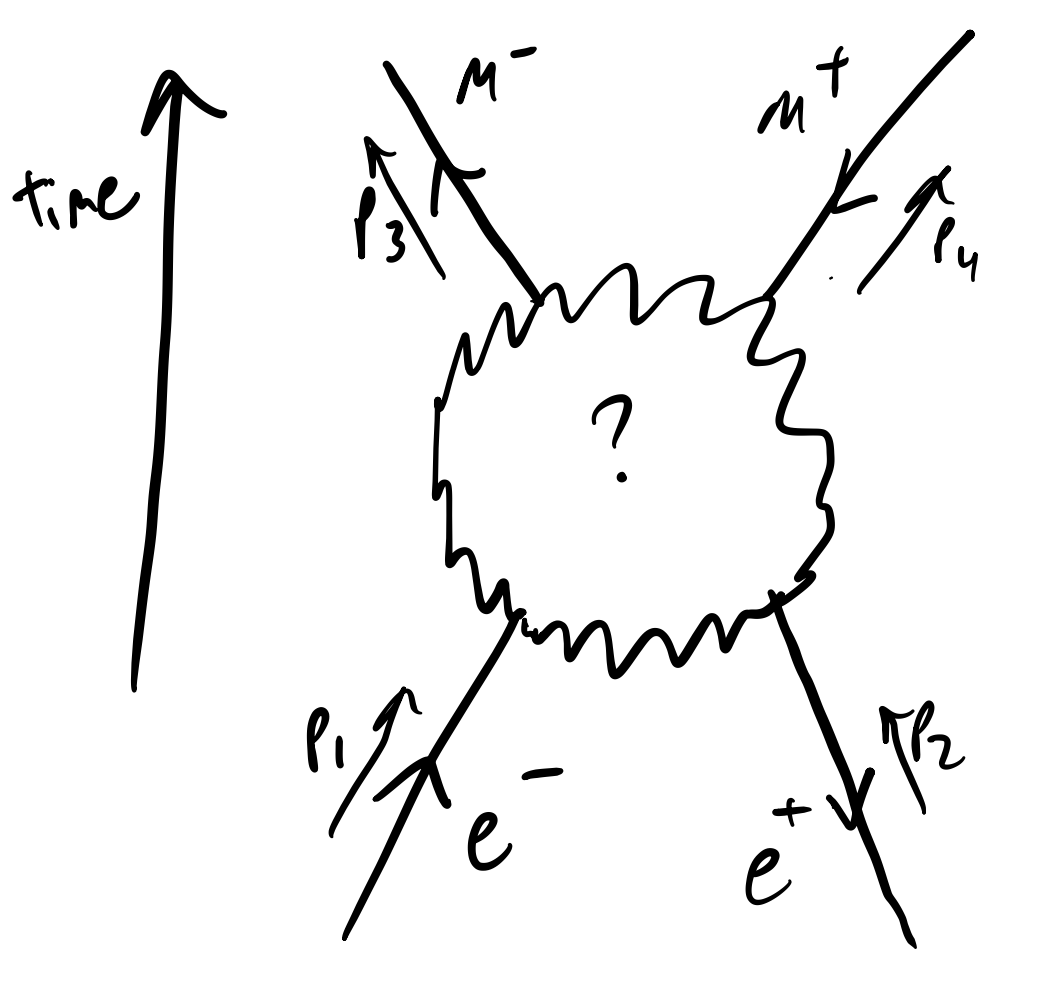
\includegraphics[scale=0.35]{Lectures/Images/lec13-mumuee.png}
\end{center}

The action of our system is:
\begin{equation}
    S = \int \bar{\psi}_e(i\slashed{D} - m_e)\psi_e + \bar{\psi}_\mu(i\slashed{D} - m_\mu)\psi_\mu - \frac{1}{4}F^2
\end{equation}
with:
\begin{equation}
    D_\mu \psi \p_\mu \psi + i e A_\mu \psi
\end{equation}
The LSZ formula tells us how to relate $\mathcal{M}$ to a connected 4-point function:
\begin{equation}
    i\mathcal{M} = i^4[(-\slashed{p}_4 + m)v_4]_\delta[\bar{u}_3(\slashed{p}_3 + m_\mu)]_\gamma\avg{\mathcal{T}\bar{\psi}^\mu_\delta(p_4)\psi^\mu_\gamma(p_3)\psi^e_\beta(p_2)\bar{\psi}^e_\alpha(p_1)}_c[\bar{v}_2(-\slashed{p}_2 + m)]_\beta[(\slashed{p}_1 + m)u_1]_\alpha
\end{equation}
Now, we calculate the correlation function using our knowledge of QED. The electrons and muons are connected via the photon field, which they are both coupled to. We will use the vertex:
\begin{equation}
    S_{\text{int}} = -e\int A_\nu(\bar{\psi}_e\gamma^\nu \psi_e + \bar{\psi}_\mu \gamma^\mu \psi_\mu)
\end{equation}
We will go to second order (intuitively - we need two powers in order to connect the $\psi_e$ and $\psi_\mu$ fields), and study the cross-terms:
\begin{equation}
    \frac{i^2}{2}S_{\text{int}}^2 = -\frac{e^2}{2}\int A \cdot (j_e + j_\mu)\int A\cdot (j_e + j_\mu) \supset -e^2\int A\cdot j_e\int A\cdot j_\mu
\end{equation}
We can drop the $(Aj_e)^2, (Aj_\mu)^2$ terms as they do not contribute to our observable of interest.

\begin{center}
    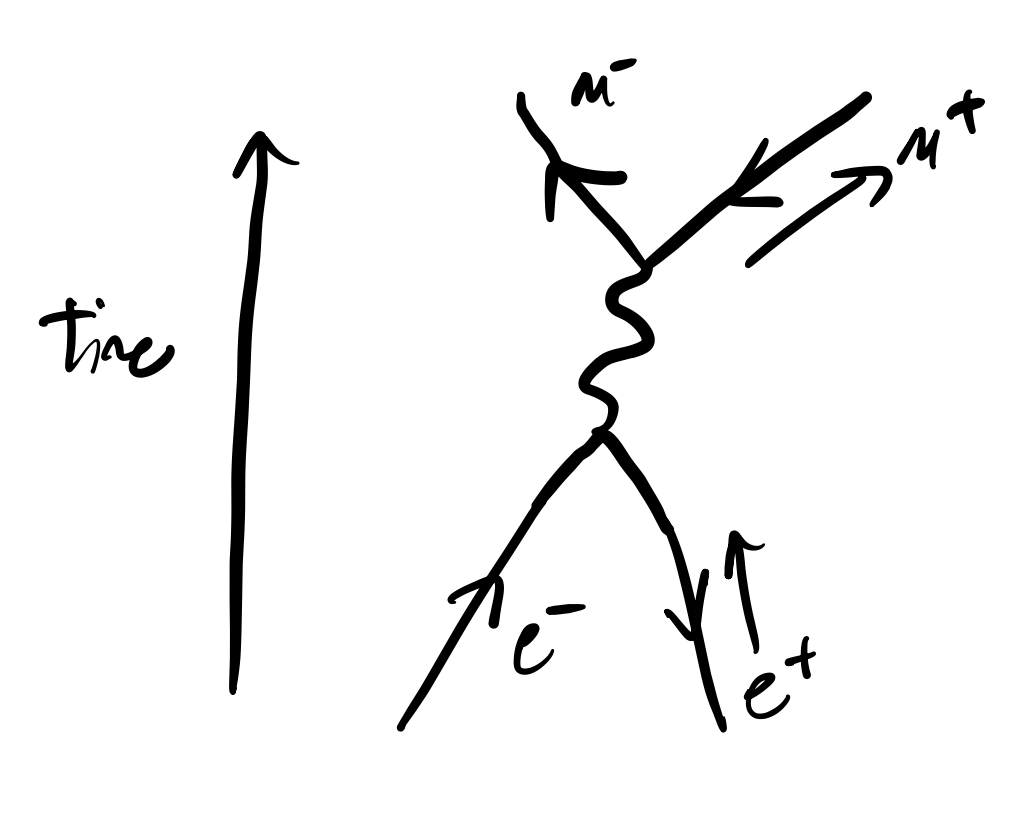
\includegraphics[scale=0.35]{Lectures/Images/lec13-mumueeschannel.png}
\end{center}

The leading contribution is thus:
\begin{equation}
    \avg{\bar{\psi}^\mu_\delta \psi^\mu_\gamma \psi^e_\beta \bar{\psi}^e_\alpha} = -e^2\avg{(\int A_\rho \bar{\psi}_\mu \gamma^\rho \psi_\mu)\bar{\psi}^\mu_\delta(p_4)\psi_\gamma^\mu(p_3)\psi_\beta^e(p_2)\bar{\psi}^e_\alpha(p_1)(\int A_\lambda \bar{\psi}^e \gamma^\lambda \psi^e)}_{\text{free}}
\end{equation}
and now we evaluate this via Wick contractions in the free theory; electrons must contract with electrons and muons must contract with muons. We contract $\psi^e$ with $\bar{\psi}_\alpha^e(p_1)$  (two exchanges so no minus) and $\psi^e_\beta(p_2)$ with $\bar{\psi}^e$, which yields:
\begin{equation}
    [G(-p_2)\gamma^\lambda G(p_1)]_{\beta\alpha}
\end{equation}
Doing the same story on the left with the muons (note there is now a minus sign to fermion exchanges), we get:
\begin{equation}
    -[G(-p_3)\gamma^\rho G(p_4)]_{\gamma\delta}
\end{equation}
Finally we contract the photons, and so at the end of the day we end up with (note that this was the unique possible choice of contractions):
\begin{equation}
    \avg{\bar{\psi}^\mu_\delta \psi^\mu_\gamma \psi^e_\beta \bar{\psi}^e_\alpha} = +e^2[G(-p_3)\gamma^\rho G(p_4)]_{\gamma\delta}G_{\rho\lambda}(p_1 + p_2)[G(-p_2)\gamma^\lambda G(p_1)]_{\beta\alpha}
\end{equation}
This is the expression for the 4-point function. Dotting it with the $(\slashed{p} + m)$ factors will simplify things because the Green's function is precisely the inverse!
\begin{equation}\label{eq:eemumu}
    \begin{split}
        i\mathcal{M} &= e^2(\bar{u}_3\gamma^\rho v_4)G_{\rho\lambda}(p_1 + p_2)(\bar{v}_2\gamma^\lambda u_1)
        \\ &= e^2(\bar{u}_3\gamma^\rho v_4)\frac{-i}{(p_1 + p_2)^2}(\eta_{\rho\lambda} + (\xi - 1)\frac{(p_1 + p_2)_{\rho}(p_1 + p_2)_\lambda}{(p_1 + p_2)^2})(\bar{v}_2\gamma^\lambda u_1)
        \\ &= \frac{ie^2}{s}(\bar{u}_3\gamma^\rho v_4)(\bar{v}_2\gamma_\rho u_1)
    \end{split}
\end{equation}
where $u_i = u_{s_i}(p_i)$, and in the third equality we use the fact that $\bar{v}_2(\slashed{p}_1 + \slashed{p}_2)u_1 = \bar{v}_2(-m + m)u_1 = 0$ to kill the $\xi$-dependent term. In the last equality we have recalled the definition of the Mandelstam variable $(p_1 + p_2)^2 = -s$.

\subsection{Comparing to the scalar, $e^-e^+ \to e^-e^+$ scattering}

Compare this to the scattering we found for the scalar:

\begin{center}
    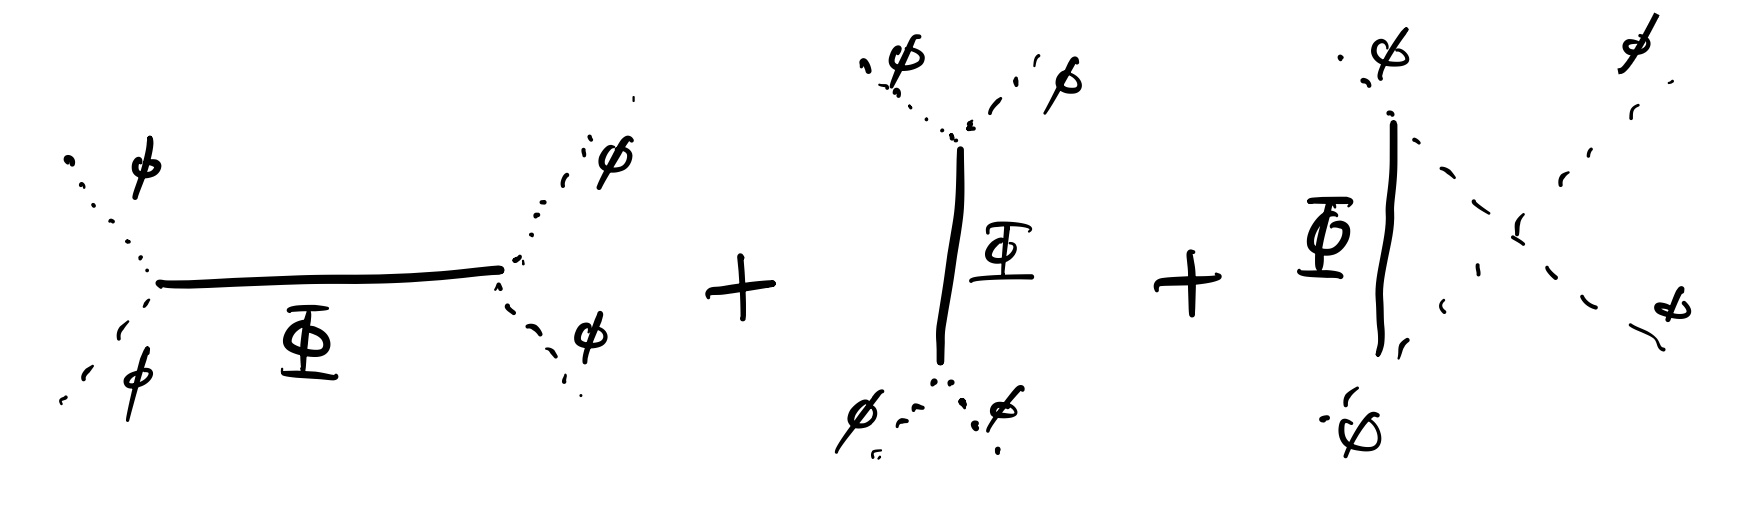
\includegraphics[scale=0.35]{Lectures/Images/lec13-scalarscatter.png}
\end{center}

where:
\begin{equation}
    \mathcal{M} \sim g^2\left(\frac{1}{s + M^2} + \frac{1}{t + M^2} + \frac{1}{u + M^2}\right)
\end{equation}
we note that with our QED scattering, the only contribution is from the $s$-channel, and since the photon is massless we do not have $M^2$ terms as we did for the massive ($\Phi$)-scalar mediated scattering. The third difference is that we have the $u/v$s which depend on the external spin and momenta.

\begin{center}
    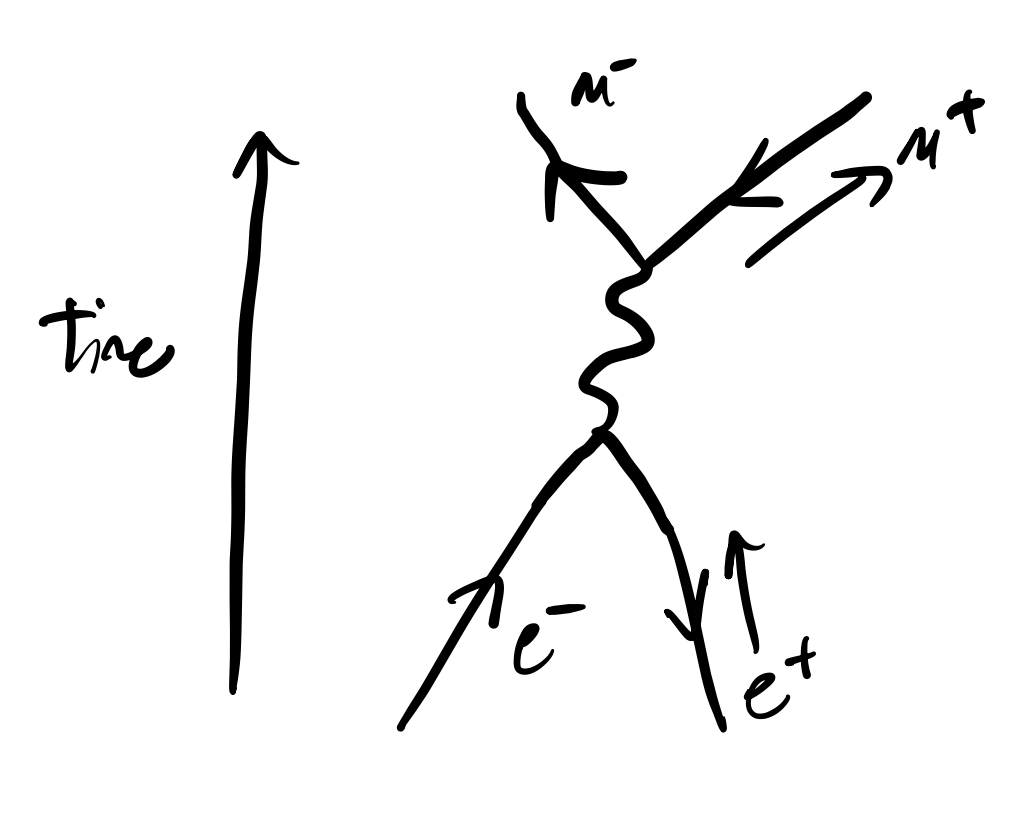
\includegraphics[scale=0.35]{Lectures/Images/lec13-mumueeschannel.png}
\end{center}

What about $e^-e^+ \to e^-e^+$ scattering? The same diagram is allowed, but there is another allowed diagram now coming from the fact that the we have two electron vertices (we get a $t$-channel  $t = -(p_1 - p_3)^2$ in addition to the $s$ channel $s = -(p_1 + p_2)^2$). This comes out of the Wick contractions, but pictorially we imagine that this second diagram corresponds to the electron staying as an electron, but radiating a photon which hits an incoming positron (as opposed to the $s$-channel diagram, which corresponds to an electron/positron pair ``becoming'' a muon/antimuon pair)

\begin{center}
    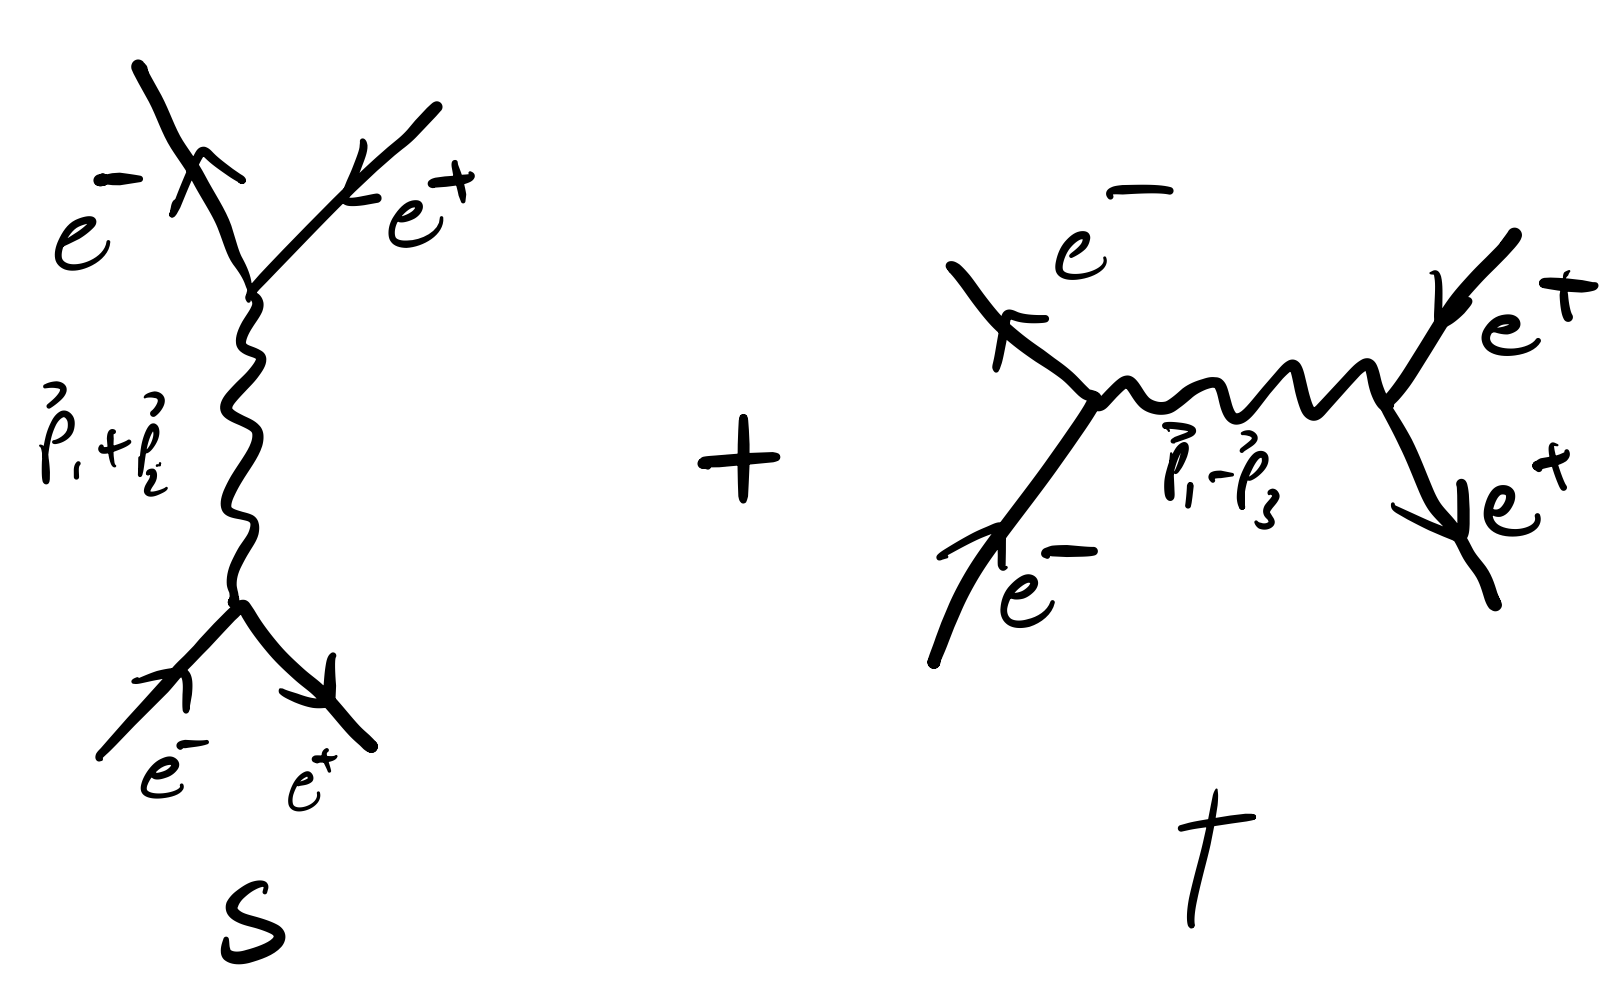
\includegraphics[scale=0.35]{Lectures/Images/lec13-stchannels.png}
\end{center}

The $u$-channel diagram below is not allowed as it has $\psi\psi A_\mu$:

\begin{center}
    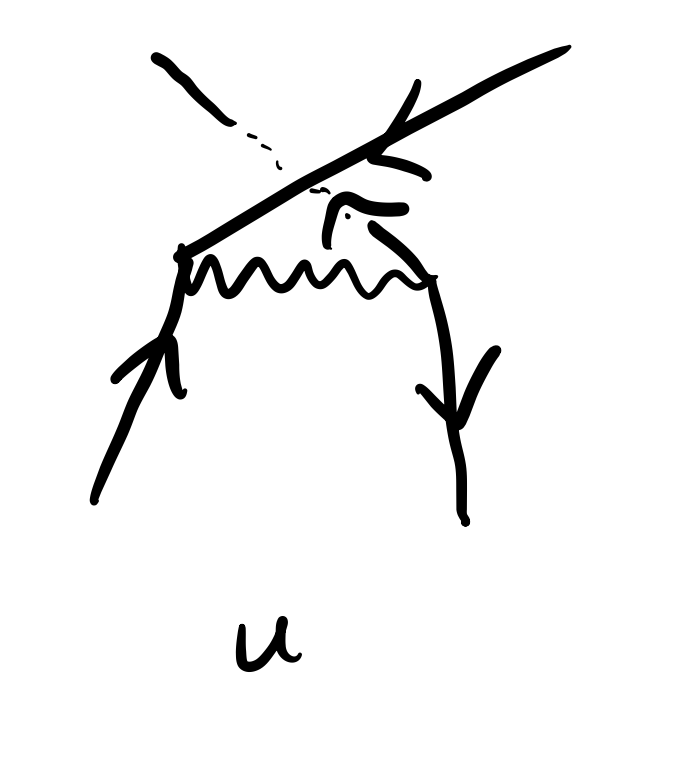
\includegraphics[scale=0.35]{Lectures/Images/lec13-uchannel.png}
\end{center}

So in summary we expect:
\begin{equation}
    \mathcal{M}_{e^-e^+ \to e^-e^+} = \frac{e^2}{s}(\bar{u}_3\gamma_\rho v_4)(\bar{v}_2\gamma^\rho u_1) + \frac{e^2}{t}(\bar{v}_2\gamma^\rho v_4)(\bar{u}_3\gamma_\rho u_1)
\end{equation}
and you check this on the homework.

\subsection{$e^+e^-\to\mu^-\mu^+$ - Summing over spins}
Going back to our result for the $e^+e^-\to\mu^-\mu^+$, if we know the momenta and all the spins, our result Eq. \eqref{eq:eemumu} is the final answer. A simpler answer arises if we sum over spins. This is also experimentally relevant if the spin of the particles is not measured.

The probability of an event is $\propto \abs{\mathcal{M}}^2$. Let's sum the probability for any outgoing set of spins:
\begin{equation}
    \abs{\mathcal{M}}^2 = \frac{e^4}{s^2}(\bar{u}_3\gamma^\rho v_4)(\bar{v}_4\gamma^\lambda u_3)(\bar{v}_2\gamma_\rho u_1)(\bar{u}_1\gamma_\lambda v_2)
\end{equation}
Let's sum over the outgoing states $s_3, s_4$ using the completeness relations:
\begin{equation}
    \sum_{s_3 = \pm}u_{s_3}(\v{p}_3)\bar{u}_{s_3}(\v{p}_3) = (-\slashed{p}_3 + M)
\end{equation}
\begin{equation}
    \sum_{s_4 = \pm}v_{s_4}(\v{p}_4)\bar{v}_{s_4}(\v{p}_4) = (\slashed{p}_4 + M)
\end{equation}
with $M = m_\mu$. We can now convert the sum over spins into taking the trace of a matrix:
\begin{equation}
    \sum_{s_3, s_4}\abs{\mathcal{M}}^2 = \frac{e^4}{s^2}\text{Tr}(\gamma^\rho(\slashed{p}_4 + M)\gamma^\lambda(\slashed{p}_3 - M))(\bar{v}_2\gamma_\rho u_1)(\bar{u}_1\gamma_\lambda v_2)
\end{equation}
Now we also average over all incoming spins $\frac{1}{4}\sum_{s_1, s_2}$:
\begin{equation}
    \frac{1}{4}\sum_{s}\abs{M}^2 = \frac{e^2}{s^2}\Tr(\gamma^\rho (\slashed{p}_4 + M)\gamma^\lambda(\slashed{p}_3 - M))\Tr(\gamma_\rho(\slashed{p}_1 - m)\gamma_\lambda(\slashed{p}_2 + m))
\end{equation}
with $m = m_e$. Now let's deal with the traces:
\begin{equation}
    \begin{split}
        \Tr(\gamma^\rho (\slashed{q} + M)\gamma^\lambda(\slashed{k} - M)) &= -m^2\Tr(\gamma^\rho\gamma^\lambda) + q_\alpha k_\beta\Tr(\gamma^\rho\gamma^\alpha\gamma^\lambda\gamma^\beta)
        \\ &= 4m^2\eta^{\rho\lambda} + 4(q^\rho k^\lambda + q^\lambda k^\rho - kq\eta^{\rho\lambda})
    \end{split}
\end{equation}
We have two traces, and the results are subsequently contracted, so:
\begin{equation}
    \begin{split}
        \frac{1}{4}\frac{1}{4}\Tr(\ldots) \Tr(\ldots) &= [M^2\eta^{\rho\lambda} + p_3^\lambda p_4^\rho + p_3^\rho p_4^\lambda - \eta^{\rho\lambda}p_3\cdot p_4][m^2\eta_{\rho\lambda} + (p^1_\rho p^2_\lambda + p^1_\lambda p^2_\rho + p^1 \cdot p^2 \eta_{\lambda\rho})]
        \\ &= 4m^2M^2 + M^2(-2)p_1 \cdot p_2 + m^2(-2)p_3 \cdot p_4 + 2(p_3 \cdot p_1) (p_2 \cdot p_4) + 2(p_3 \cdot p_2)(p_1 \cdot p_4) - 4(p_3 \cdot p_4)(p_1 \cdot p_2) + 4(p_3 \cdot p_4)(p_1 \cdot p_2)
        \\ &= 4mM^2 - 2(M^2p_{12} + m^2p_{34}) + 2(p_{13}p_{24} + p_{14}p_{23})
    \end{split}
\end{equation}
Thus the probability of scattering, ignoring spin, is proportional to:
\begin{equation}
    \frac{1}{4}\sum_{s_1s_2s_3s_4}\abs{\mathcal{M}}^2 = \frac{8e^2}{s^2}[2m^2M^2 - (M^2p_{12} + m^2p_{34}) + (p_{13}p_{24} + p_{14}p_{23})]
\end{equation}
Indeed this is independent of spin and only depends on Lorentz-invariant contractions of four-momenta $p_{ij} = p_i \cdot p_j$. Finally, let us convert to Mandelstam variables:
\begin{equation}
    s = -(p_1 + p_2)^2 = m^2 - 2p_{12} \stackrel{\text{p}-conservation}{=} -(p_3 + p_4)^2 = 2M^2 - 2p_{34}
\end{equation}
\begin{equation}
    t = -(p_1 - p_3)^2 = m^2 + M^2 + 2p_{13} \stackrel{\text{p}-conservation}{=} -(p_2 - p_4) = m^2 + M^2 + 2p_{24}
\end{equation}
\begin{equation}
    u = -(p_2 - p_4)^2 = m^2 + M^2 + 2p_{14} \stackrel{\text{p}-conservation}{=} -(p_1 - p_3)^2 = m^2 + M^2 + 2p_{13}
\end{equation}
Thus replacing the $p_{ij}$ in our probability expression:
\begin{equation}
    \boxed{\frac{1}{4}\sum_{s_1,s_2,s_3,s_4}\abs{\mathcal{M}}^2 = \frac{8e^2}{s^2}[t^2+ u^2 + 4s(m^2 + M^2) - 2(m^2 + M^2)^2]}
\end{equation}
Last quarter, we saw how to get a differential cross section out of this; as we obtained for scalars; at high-energies with $p \gg M,m$ this yields:
\begin{equation}
    \dod{\sigma}{\Omega} = \text{Const.}\cdot\frac{e^4}{E_{\text{CM}}^2}(1 + \cos^2\theta)
\end{equation}

\begin{center}
    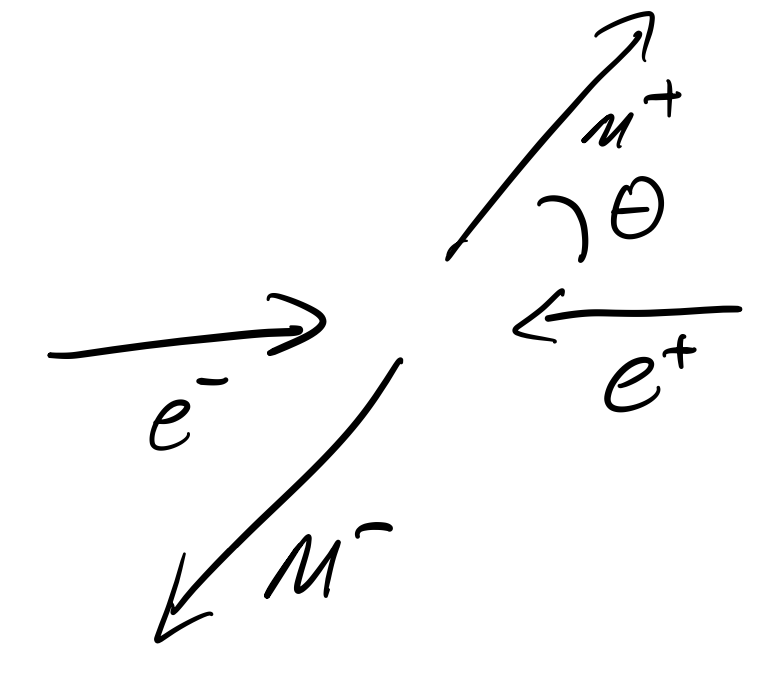
\includegraphics[scale=0.35]{Lectures/Images/lec13-angledependence.png}
\end{center}

See Schwartz (13.78) for details. What is the intuition for this expression? For scalars we found that $M = \lambda$ and $\dod{\sigma}{\Omega} = \frac{\lambda^2}{E_{CM}^2}$, coming from:

\begin{center}
    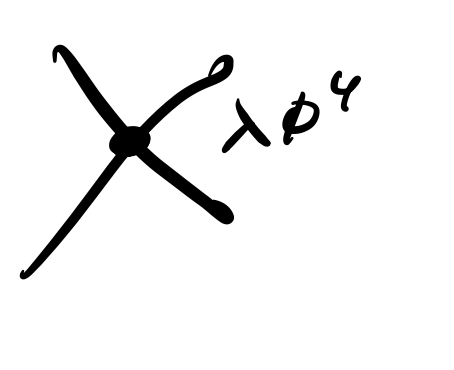
\includegraphics[scale=0.35]{Lectures/Images/lec13-scalarvertex.png}
\end{center}

Now, we have angle dependence. Why? It has to do with the spin. Because the electron/positron pair must create a photon to mediate their interaction, we need their helicities to align a helicity-1 photon state. If the helicities are all pointing out of the page/normal to the direction of propagation, we have exactly what we want. If instead they point in the plane of the collision, the helicities of muon no longer quite align and hence we get a $\propto (\cos\theta)^2$ dependence.

\begin{center}
    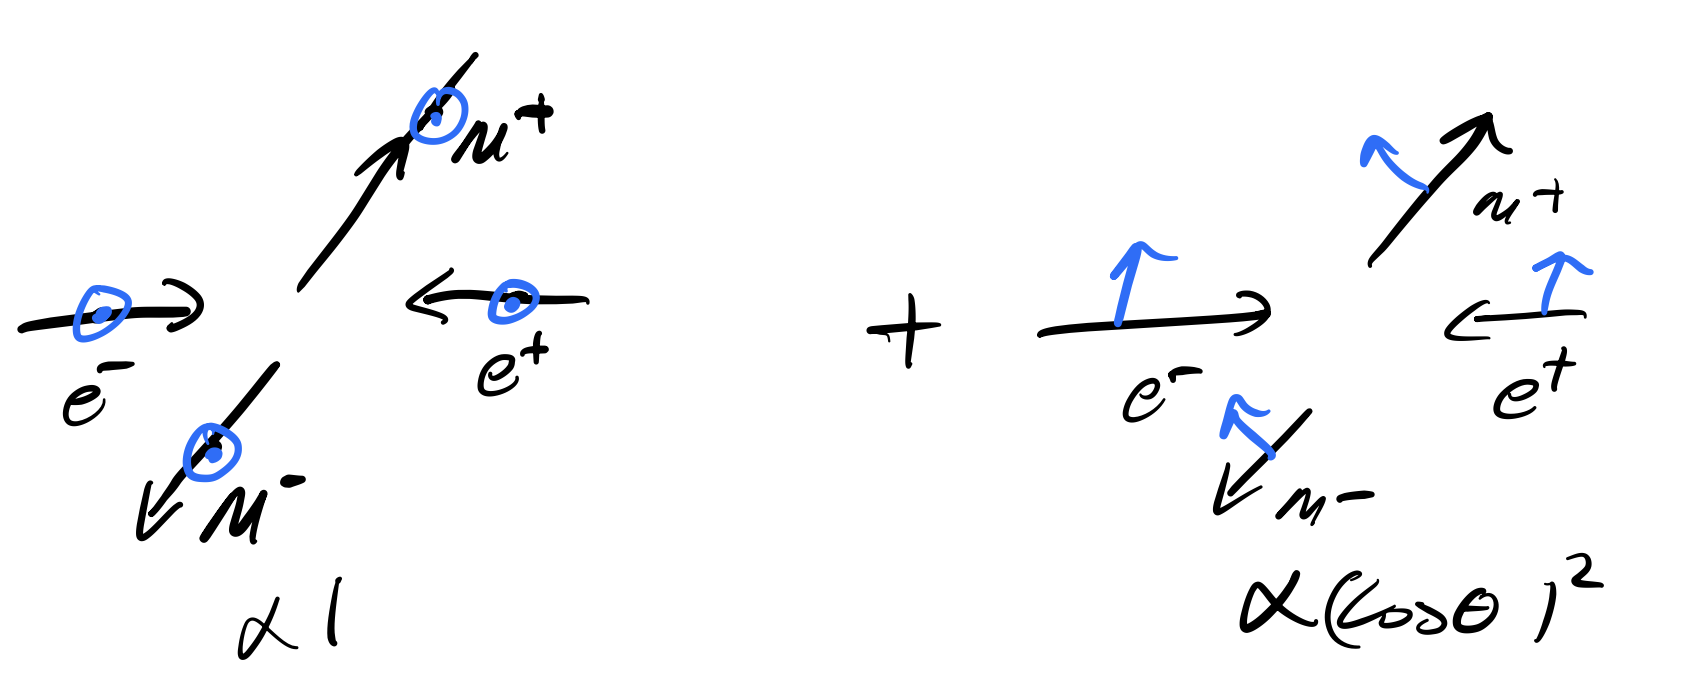
\includegraphics[scale=0.35]{Lectures/Images/lec13-twoparts.png}
\end{center}

\section{Soft and Collinear divergences in QED}

We're about to begin out last topic! It's slightly advanced - it's dealing with the fact that $S$-matrix cannot be formally defined in a theory without a mass gap. This technique is crucial if you continue on in particle physics, physics of jets, colliders etc. In QED, the photon is a massless particle, causing the problem; the precise issue is that single particle states cannot be distinguished from the multi-particle continuum; few particle ``out'' states look the same as few particle ``out'' states + soft/low-energy photons.

\subsection{Sketching the problem}

The dispersion if we only had electron looks like:

\begin{center}
    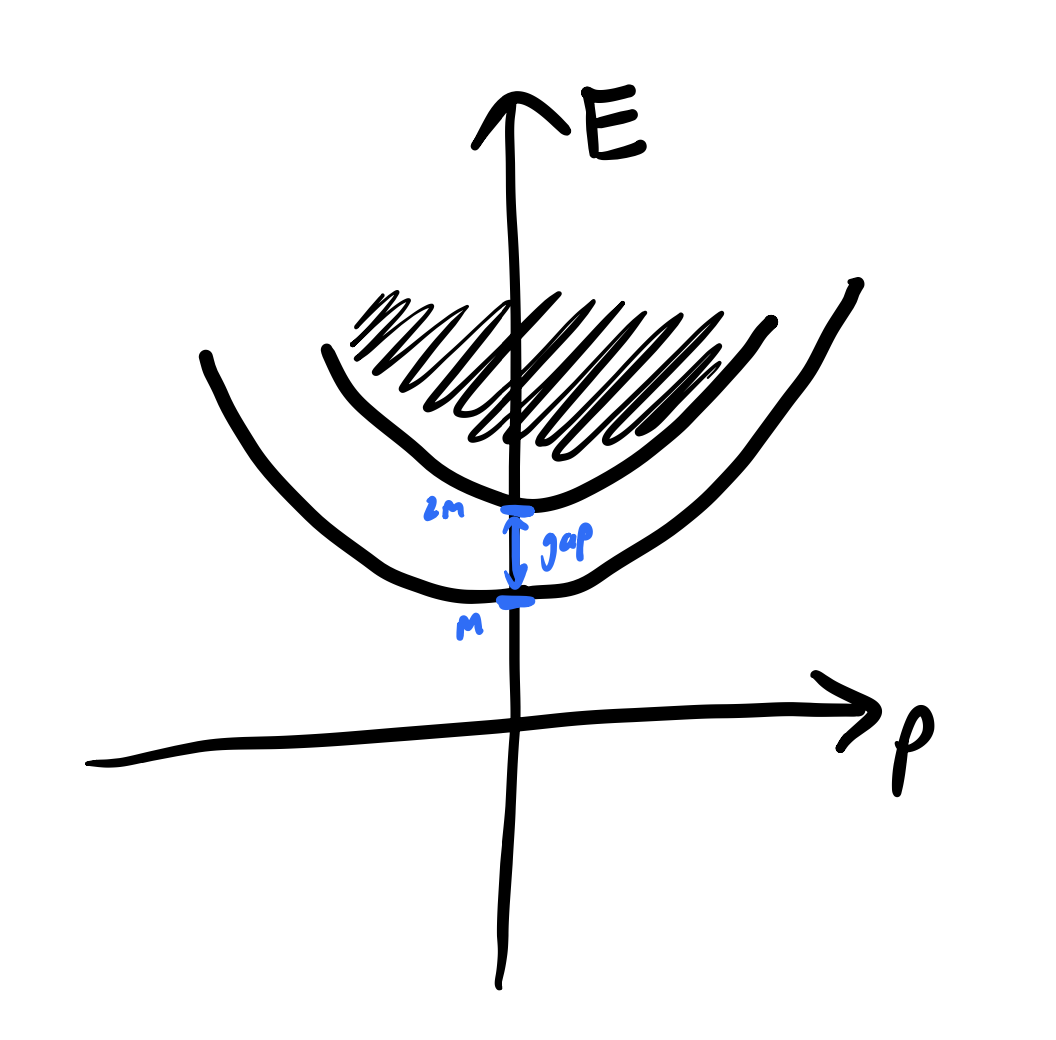
\includegraphics[scale=0.35]{Lectures/Images/lec14-massgap.png}
\end{center}

i.e. the theory has a gap, allowing us to define the $S$-matrix. But in QED, we now have photons, so we have a continuum of electron + photon states:

\begin{center}
    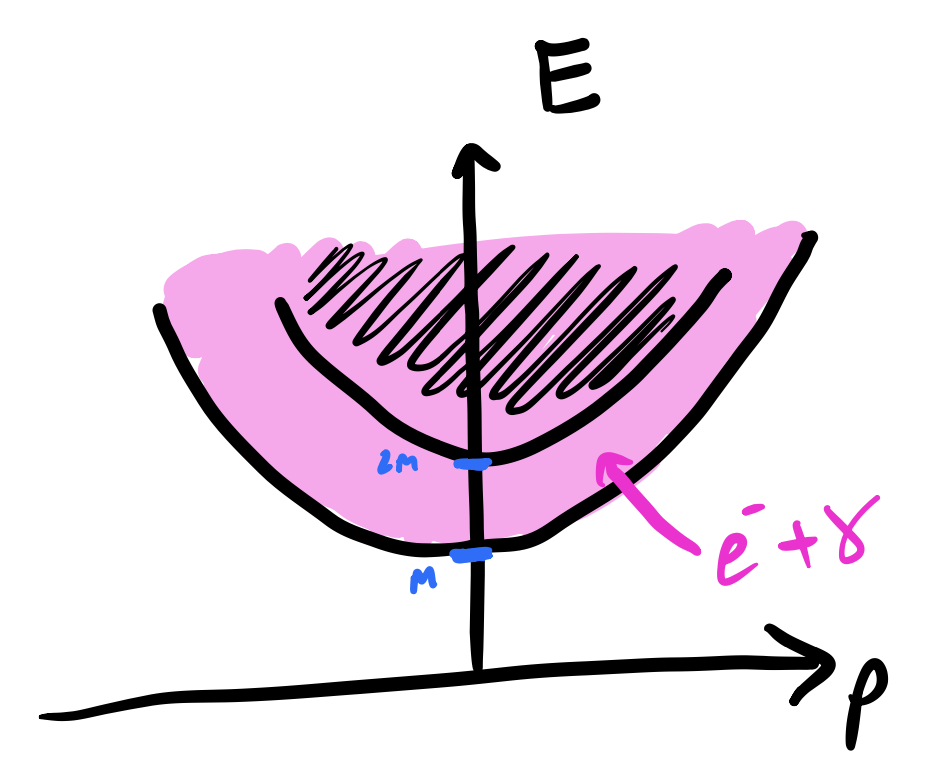
\includegraphics[scale=0.35]{Lectures/Images/lec14-nogap.png}
\end{center}

In equations, an $e^-$ at momentum $\v{p}$ has energy:
\begin{equation}
    E = \sqrt{\v{p}^2 + m^2}
\end{equation}

And a $e^- + \gamma$ state at total momentum $\v{p}$ has $e^-$ with momentum $\v{p} - \v{k}$ and $\gamma$ with momentum $\v{k}$, so the energy is:
\begin{equation}
    E = \sqrt{(\v{p}-\v{k})^2 + m^2} + \abs{\v{k}} = \sqrt{\v{p}^2 + m^2} + \mathcal{O}(\abs{\v{k}})
\end{equation}
and crucially, there is no gap because $\v{k} \to 0$ continuously in infinite volume. For finite size, $k = \frac{2\pi}{L}$ becomes quantized; this is a hint for the resolution.

One cannot ignore this issue; loop corrections to matrix elements will have IR divergences, also known as ``soft'' divergences. These are divergences of a very different type as UV divergences we have seen prior. Either we have an EFT which the UV divergence indicates that there is a scale which the theory breaks down, or the theory is UV-complete in which the case that the divergences can be regulated/removed by counterterms.

What does the IR divergence tell us about the theory? It doesn't tell us that the theory has a problem (indeed we found that QED is IR-free from our RG analysis)! Rather, it tells us that the observables we are choosing are bad. Here, we will see that the divergences arise in the step of putting the external particles/legs on shell in LSZ. The ``off-shell'' correlators that we have been studying (e.g. $\avg{\mathcal{T}\ldots}_c$) that we have been studying are always well-defined; it is only when we take specific limits (in order to put external legs on shell) that problems arise. 

These will get resolved if we accept the fact that we cannot distinguish $\ket{\psi}$ of interest with $\ket{\psi + \text{soft photons}}$. Fortunately, we will not have to consider an arbitrary number of soft photons. For example at 1-loop order the cross-section $\sigma$ is finite if we include states with one extra soft photon. Diagramatically:

\begin{center}
    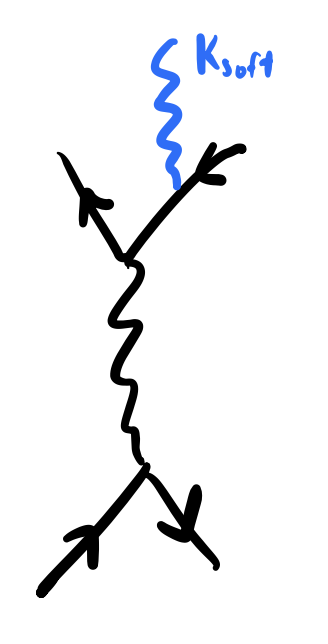
\includegraphics[scale=0.35]{Lectures/Images/lec14-singlesoft.png}
\end{center}

Specifically, we will see that the cross-section:
\begin{equation}
    \sigma(e^-e^+ \to \mu^-\mu^+) + \sigma(e^-e^+ \to \mu^-\mu^+\gamma)
\end{equation}
is IR finite. At higher orders, diagrams with more soft $\gamma$s must be included - we do not need to include them all at once because we look at perturbation theory in powers of $e$. Note that the calculation we did last lecture was at tree-level and hence we did not have to worry about soft divergences there.

\begin{center}
    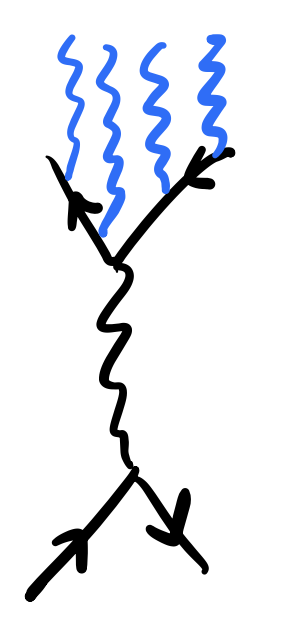
\includegraphics[scale=0.35]{Lectures/Images/lec14-multisoft.png}
\end{center}

We use the above scattering cross section as an example, but really, IR divergences are everywhere.

\begin{center}
    
\includegraphics[scale=0.35]{Lectures/Images/lec14-everywhere.jpg}
\end{center}

It is easy to see that there will be an IR issue in the diagram:

\begin{center}
    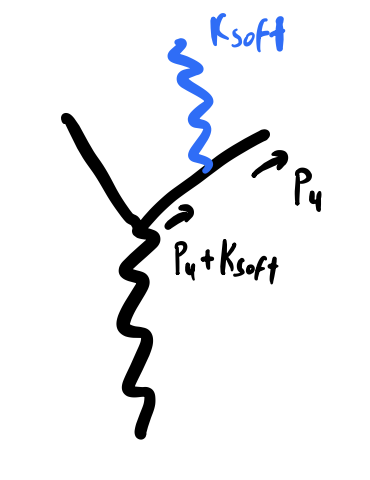
\includegraphics[scale=0.35]{Lectures/Images/lec14-softzoom.png}
\end{center}

Because this diagram contains the propagator:
\begin{equation}
    G_\psi(p_4 + k_{\text{soft}}) = \frac{-i(M + \slashed{p}_4 + \slashed{k}_{\text{soft}})}{(p_4 + k_{\text{soft}})^2 + M^2} \stackrel{p_4^2 = -M}{=} \frac{-i(\ldots)}{k_{\text{soft}}^2 + 2k_{\text{soft}} \cdot p_4} \sim \frac{1}{k_{\text{soft}} \cdot p_4}
\end{equation}
which diverges as $k_{\text{soft}} \to 0$.

\subsection{One-loop corrections at $e^-e^+ \to \mu^-\mu^+$}
What are the 1-loop corrections to $\mathcal{M}(e^-e^+ \to \mu^-\mu^+)$? We have the 6 diagrams (in addition to the single tree-level diagram we had previously):
\begin{center}
    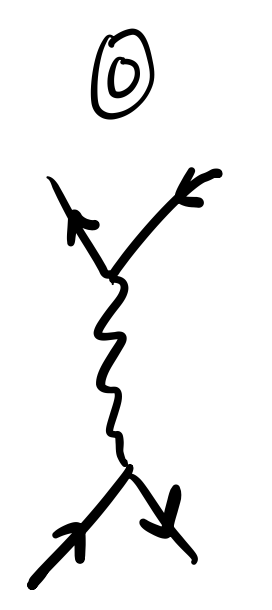
\includegraphics[scale=0.35]{Lectures/Images/lec14-treediagram.png}
\end{center}
\begin{center}
    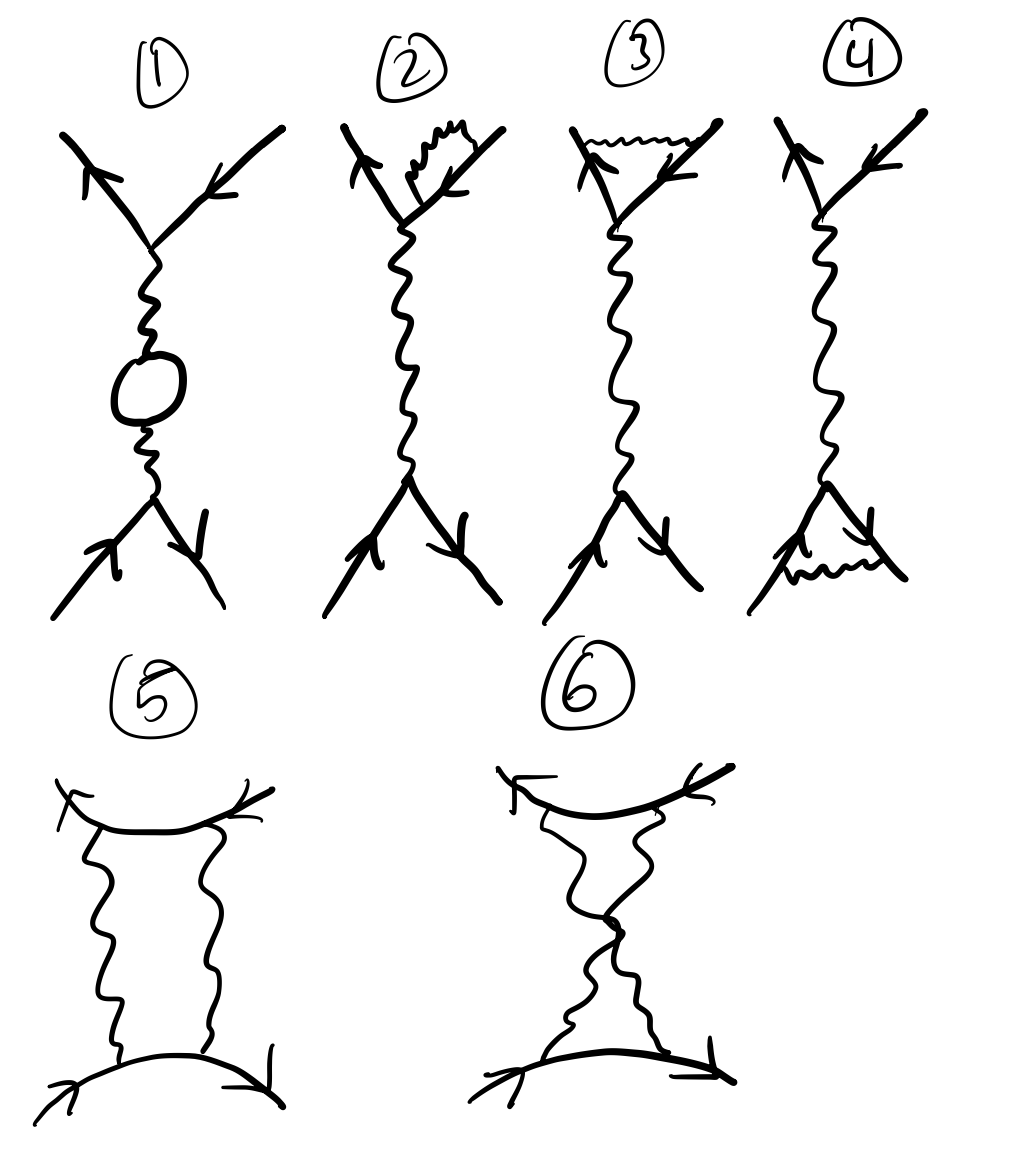
\includegraphics[scale=0.35]{Lectures/Images/lec14-oneloopdiagrams.png}
\end{center}

(2) drops out/does not contribute to the cross-section as the leg gets amputated. But this still looks pretty bad - 5 diagrams to calculate. But let's be a bit clever. Let's slightly modify QED and assign different charges $Q_e, Q_\mu \neq 1$ to the electron and muon. The reason to do this is:
\begin{equation}
    S_{\text{int}} = -e\int A_\nu(Q_e\bar{\psi}_e\gamma^\nu \psi_e + Q_\mu \bar{\psi}_\mu \gamma^\nu \psi_\mu)
\end{equation}
What is the motivation? Divergences in the electron and muon degrees of freedom have to cancel independently. Although we are interested in $Q_e = Q_\mu = 1$, this property nontheless carries over.

We start with looking at the effect the tree-level $\mathcal{M}_0$, which looking at diagram (0) we see $\mathcal{M}_0 \propto Q_eQ_\mu$ (each fermion vertex contributes a power of the respective charge). Let's look at the other diagrams. (1) is proportional to $Q_eQ_\mu Q_x^2$ because the fermion correction to the photon energy could come from any mystery fermion $x$ (it thus must cancel itself). (2) is not in $\mathcal{M}$. (3) is proportional to $Q_eQ_\mu^3$, (4) is proportional to $Q_e^3Q_\mu$, (5) is proportional to $Q_e^2Q_\mu^2$, and (6) is proportional to $Q_e^2Q_\mu^2$.

IR divergences proportional to any $Q_e^{c_e}Q_{\mu}^{c_\mu}$ have to cancel independently. We will focus on the $Q_eQ_\mu^3$ part/diagram (3) and look at its contribution to $\sigma \propto \abs{\mathcal{M}}^2$:

\begin{center}
    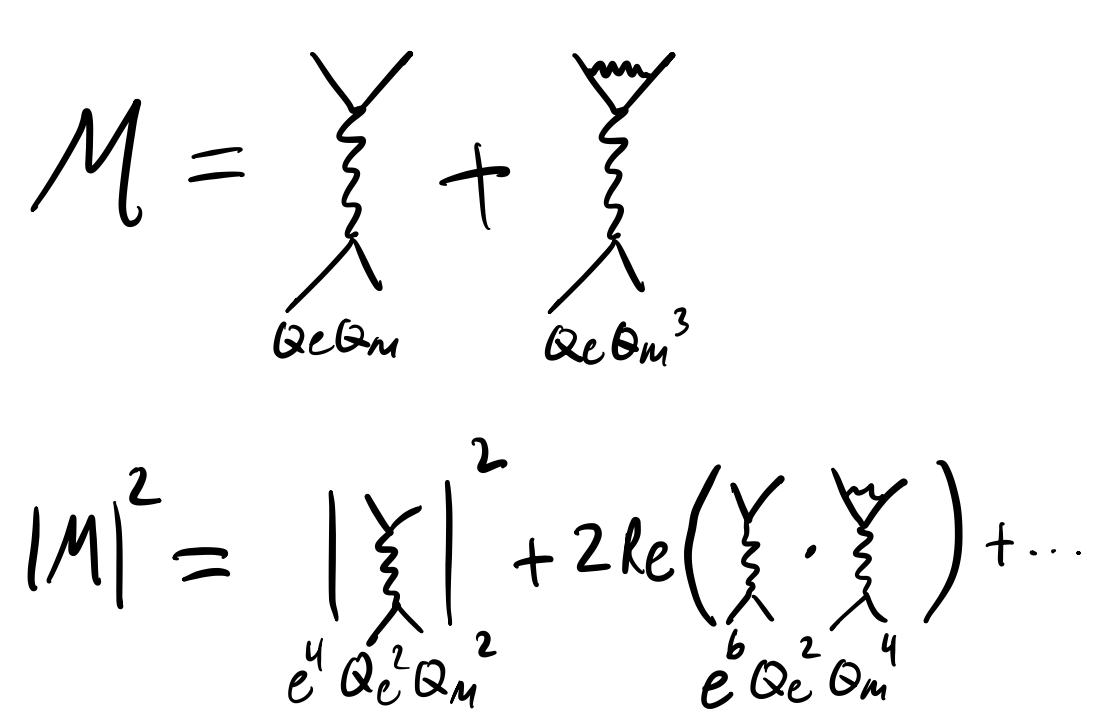
\includegraphics[scale=0.35]{Lectures/Images/lec14-oneloopcrosssection.png}
\end{center}

This correction indeed competes with the $\sigma(e^-e^+ \to \mu^-\mu^+\gamma)$ cross-section, because looking at the diagrams with the soft photon:

\begin{center}
    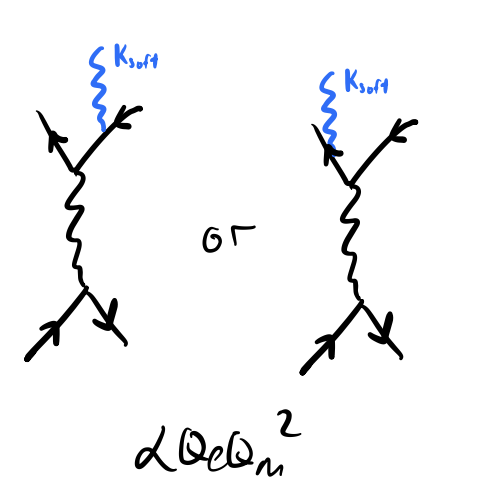
\includegraphics[scale=0.35]{Lectures/Images/lec14-softphotondiagrams.png}
\end{center}

(note that we can only put the soft photon on the muon leg) we see:
\begin{equation}
    \sigma(e^-e^+ \to \mu^-\mu^+\gamma) \sim \abs{\mathcal{M}}^2 \sim Q_e^2Q_\mu^4
\end{equation}

This trick with introducing fictitious charges is nice because it simplifies the analysis to specific diagrams. Let's now hone in and see how the divergences cancel.

\subsection{Computing the one-loop correction}
So, the only loop diagram we will have to consider is (3). The leading diagram is:

\begin{center}
    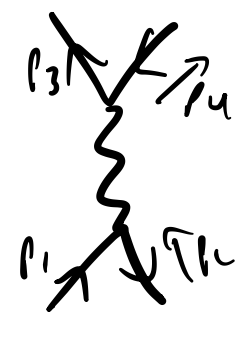
\includegraphics[scale=0.35]{Lectures/Images/lec14-treemomenta.png}
\end{center}

\begin{equation}
    i\mathcal{M}_0 = \frac{ie^2}{s}(\bar{v}_2\gamma^\rho u_1)(\bar{u}_3\gamma_\rho v_4)
\end{equation}

the 1-loop correction is:'

\begin{center}
    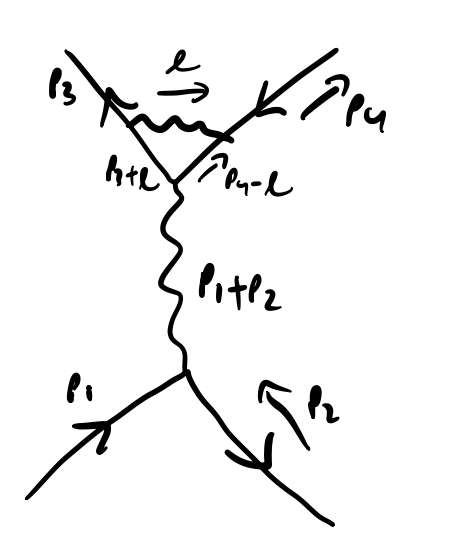
\includegraphics[scale=0.35]{Lectures/Images/lec14-oneloopmomenta.png}
\end{center}

\begin{equation}
    i\mathcal{M}_{\text{1-loop}} =  \frac{ie^2}{s}(\bar{v}_2\gamma^\rho u_1)(\bar{u}_3\Gamma_\rho v_4)
\end{equation}
with:
\begin{equation}
    \Gamma_\rho = \avg{j_\rho(p_1 + p_2)\psi\bar{\psi}(-p_4)}_{\text{amputated, 1-loop}}
\end{equation}

this is just an old friend! We will notice that this actually has IR divergences when we put the external legs on-shell, as is required by LSZ. Why didn't we notice? In RG we didn't put the external legs on shell, so we didn't see it. When we computed the electron dipole moment, we only looked at the terms which were IR safe. This is why many of the early calculations were successful, even though they didn't yet know how to handle these IR singularities.

Let's compute the diagram:

\begin{center}
    \includegraphics[scale=0.35]{Lectures/Images/lec14-oneloopmomentazoom.png}
\end{center}

We then have:
\begin{equation}
    \Gamma_\rho = \frac{(-ie)^2}{2}\avg{(\bar{\psi}\gamma^\rho\psi)_{p_1 + p_2}(\int A_\alpha \bar{\psi}\gamma^\alpha \psi)(\int A_\beta \bar{\psi}\gamma^\beta \psi)\psi \bar{\psi}(-p_4)}
\end{equation}
Wick contractions in order to get a connected diagram:

\begin{center}
    \includegraphics[scale=0.35]{Lectures/Images/lec14-pairings.png}
\end{center}

Thus:
\begin{equation}
    \Gamma_\rho = -e^2\int_l G(p_3)\gamma^\beta G(p_3 + l)\gamma^\rho G(l - p_4)\gamma^\alpha G(-p_4)G_{\alpha\beta}(l)
\end{equation}
If we amputate the external legs:
\begin{equation}
    \Gamma_\rho = -e^2\int_l \gamma^\beta G(p_3 + l)\gamma^\rho G(l - p_4)\gamma6\alpha G_{\alpha\beta}(l)
\end{equation}
Then we are left with (recalling that $G(p) = -\frac{-i}{M - \slashed{p}} = \frac{-i(M + \slashed{p})}{p^2 + M^2}$ and $G_{\alpha\beta}(l) = \frac{-i}{l^2}\eta_{\alpha\beta}$ choosing $\xi = 1$):
\begin{equation}
    \Gamma_\rho = -ie^2\int \frac{d^4l}{(2\pi)^4}\frac{\gamma_\alpha(M + \slashed{l} + \slashed{p}_3)\gamma^\rho (M + \slashed{l} - \slashed{p}_4)\gamma^\alpha}{l^2((l + p_3)^2 + M^2)((l - p_4)^2 + M^2)}
\end{equation}
so with $p_3^2 = p_4^2 = -M^2$ (on shell) the denominator becomes $l^2(l^2 + 2l\cdot p_3)(l^2 - 2l\cdot p_4)$ so as $l \to 0$ this goes as $l^2(l\cdot p_3)(l \cdot p_4)$ which implies:
\begin{equation}
    \Gamma_\rho \sim \frac{d^4l}{l^4}
\end{equation}
which is a (log) IR divergence. We can manifestly see how this arose from setting the momenta to be on-shell. This is actually a bit too quick. The above analysis looks like just a log divergence. But actually it can be even smaller, if $l$ is collinear with $p_{3/4}$ wherein the dot product vanishes. So when we integrate, we will see additional singularities arise from collinear momenta. This will lead to $\log^2$ singularities, which cannot be resummed via RG.

Before we show that this cancels with the other diagram, we need a way to compute it. In order to do this, we need to be able to regulate it. We will choose a simple but ugly IR regulator, i.e. giving the photon a mass $m_\gamma$. A more physical (but slighty harder to work with) regulator is to put things in a finite volume which gives the photon a maximum possible wavelength. In any case, with our choice of regulator the photon propagator transforms as:
\begin{equation}
    \frac{1}{l^2} \to \frac{1}{l^2 + m_\gamma^2}
\end{equation}
Focusing on the IR divergences, take $l \ll M, p_3, p_4$. For simplicity, we further assume high-energy scattering, i.e. $p_3, p_4 \gg M$. Then:
\begin{equation}
    \Gamma \cong ie^2\int_l \frac{\gamma_\alpha\slashed{p}_3\gamma^\rho \slashed{p}_4\gamma^\alpha}{(l^2 + m_\gamma^2)(l^2 + 2l \cdot p_3)(l^2 - 2l \cdot p_4)} = ie^2\int_l \frac{2\slashed{p}_4\gamma^\rho \slashed{p}_3}{(l^2 + m_\gamma^2)(l^2 + 2l \cdot p_3)(l^2 - 2l \cdot p_4)}
\end{equation}
If we sandwich the numerator with $\bar{u}_3 (\ldots)v_4$ then:
\begin{equation}
    \begin{split}
        \bar{u}_3 2\slashed{p}_4\gamma^\rho \slashed{p}_3v_4 &= 2\bar{u}_3\slashed{p}_4 \gamma^\rho \slashed{p}_3v_4 
        \\ &= -2\bar{u}_3(2p_3^\rho \slashed{p}_4 + \slashed{p}_4\slashed{p}_3 \gamma^\rho)v_4 
        \\ &= -2\bar{u}_3(2Mp_3^\rho - \slashed{p}_3\slashed{p}_4 \gamma^\rho - 2p_3 \cdot p_4 \gamma^\rho)v_4 
        \\ &= -2\bar{u}_3(2M(p_3^\rho - p_4^\rho) + M^2\gamma^\rho - 2p_3 \cdot p_4 \gamma^\rho)v_4 
        \\ &\stackrel{p_3, p_4 \gg M}{\approx} 4p_3 \cdot p_4 \bar{u}_3v_4 = -2s\bar{u}_3v_4
    \end{split}
\end{equation}
where in the last line we use:
\begin{equation}
    s = (-p_3 + p_4)^2 = 2M^2 - 2p_3 \cdot p_4 \approx -2p_3 \cdot p_4
\end{equation}
So at the end of the day, our $\Gamma_\rho$ looks like:
\begin{equation}
    \Gamma^\rho = -2ies\int \frac{d^4l}{(2\pi)^4}\frac{1}{(l^2 + m_\gamma^2)(l^2 + 2l \cdot p_3)(l^2 - 2l \cdot p_4)}
\end{equation}
So introducing Feynman parameeters with $x = l^2  +2l\cdot p_3$ and $y = l^2 - 2l \cdot p_4$ we have:
\begin{equation}
    \begin{split}
        \Gamma^\rho &= -4ies\int_0^1dx \int_0^{1-x}dy \int_l \frac{1}{[l^2 + 2l(p_3x - p_4y) + m_\gamma^2(1-x-y)]^3} 
        \\ &= -4ies\int_0^1dx \int_0^{1-x}dy \int_l \frac{1}{[(l + p_3x - p_4y)^2 + m_\gamma^2(1-x-y) - (p_3x - p_4y)^2]^3} 
        \\ &= -4ies\int_{xy}\int_q \frac{1}{(q^2 + \Delta)^3}
    \end{split}
\end{equation}
Which we can compute via Wick rotation:
\begin{equation}
    \stackrel{\text{Wick}}{\to} 4es \int_{xy}\frac{2\pi^2}{(2\pi)^4}\int_0^\infty \frac{dq q^3}{(q^2 + \Delta)^3}
\end{equation}
So then:
\begin{equation}
    \Gamma_\rho = \frac{es}{8\pi}\int_0^1 dx \int_0^{1-x}dy \frac{1}{\Delta}
\end{equation}
We will finish the calculation next week, but the $\Delta$ is $\sim m_\gamma^2 + xys$, the first integral gives $\sim \frac{\log(\ldots x)}{x}$ and the second gives $\log^2(\ldots)$, which is how the collinear singularities manifest, as we discussed. We will see that the result is $\sim \log(\frac{s}{m_\gamma})^2$.
\section{Soft Divergences II}

\subsection{1-Loop correction to $e^+e^- \to \mu^+\mu^-$, continued}
We were computing the 1-loop correction to the $e^+e^- \to \mu^+\mu^-$ cross section:

\begin{center}
    \includegraphics[scale=0.35]{Lectures/Images/lec15-1loopdiagrams.png}
\end{center}

where we found:
\begin{equation}
    i\mathcal{M} = \frac{ie^2}{s}(\bar{v}_2\gamma^\rho u_1)(\bar{u}_3(\gamma_\rho + \Gamma_\rho)v_4)
\end{equation}
with:
\begin{equation}
    \Gamma_\rho = \left.\avg{j_\rho(p_3 + p_4)\psi\bar{\psi}(-p_4)}_{\text{amp}}\right|_{\text{1-loop}} = \gamma_\rho \frac{e^2}{8\pi^2}\int_0^1 dx\int_0^{1-x}dy \frac{s}{\Delta}
\end{equation}
with:
\begin{equation}
    \begin{split}
        \Delta = m_\gamma^2(1 - x - y) - (xp_3 - yp_4)^2 &= m_\gamma^2(1-x-y) + (x^2 + y^2)M^2 + 2p_3 \cdot p_4xy
        \\ &\approx m_\gamma^2(1-x-y) + 2p_3 \cdot p_4xy
        \\ &= m_\gamma^2(1 - x - y) - sxy
    \end{split}
\end{equation}
where we focus on high $E$ ($E \gg M$) scattering in the second-to-last line, and in the last line we use the approximate expression for the Mandelstam variable:
\begin{equation}
    s = -(p_3 + p_4)^2 = 2M^2 - 2p_3 \cdot p_4 \approx -2p_3 \cdot p_4
\end{equation}
Let's look at these final two integrals. They will do something unusual. They can be computed exactly (as you will see on PS8), and the leading $m_\gamma \to 0$ singularity is:
\begin{equation}
    \int_{xy}\frac{s}{\Delta} \approx -\frac{1}{2}(\log \frac{m_\gamma^2}{s})^2 \implies \Gamma_\rho = -\gamma_\rho\frac{e^2}{16\pi^2}(\log\frac{m_\gamma^2}{s})^2
\end{equation}
this is quite unusual. These logarithms are called the Sudhakov double-logarithm. They are unlike what we saw in RG, which were logarithms which we were able to resum.

Let's sketch the computation of this integral. If we send $m_\gamma^2 \to 0$, $\frac{1}{\Delta}$ becomes singular for $x \to 0$ or $y \to 0$. Let's take a look at these regions:
\begin{equation}
    \begin{split}
        \int_{xy}\frac{s}{\Delta} = \int_0^1 dx \int_0^{1-x}dy \frac{1}{\frac{m_\gamma^2}{s}(1-x-y) - xy} &\sim \int_0^1 dx \int_0^1 dy \frac{1}{\frac{m_\gamma^2}{s} - xy} 
        \\ &= \int_0^1dx \frac{1}{x}\left.\log(\frac{m_\gamma^2}{s} - xy)\right|_0^1
        \\ &= \int_0^1 dx \frac{1}{x}\left[\log(\frac{m_\gamma^2}{s} - x) - \log\frac{m_\gamma^2}{s}\right] 
        \\ &= \int_0^1 dx \frac{1}{x}\log(1 - \frac{s}{m_\gamma^2}x)
    \end{split}
\end{equation}
Now using the identity that $\dod{}{z}\frac{1}{2}\log^2(z) = \frac{\log z}{z}$ we find that the above integral evaluates to $\sim \frac{1}{2}\log^2$.

Hence, our matrix element becomes:
\begin{equation}
    i(\mathcal{M} + \mathcal{M}_\Gamma) = \frac{ie^2}{s}(\bar{v}_2\gamma^\rho u_1)(\bar{u}_3\gamma_\rho v_4)\left[1 - \frac{e^2}{16\pi^2}\left(\log\frac{m_\gamma^2}{s}\right)^2 + \ldots\right]
\end{equation}
where - nicely - the spins structure is exactly the same! So whatever we did for the tree level piece carries over. We thus find that:
\begin{equation}
    \sigma(e^+e^- \to \mu^+\mu^-) = \int \frac{1}{4}\sum_s \abs{\mathcal{M}}^2 d\Pi_{\text{LIPS}} = \frac{e^4}{12\pi s}\left[1 - \ldots\right]^2 = \frac{e^4}{12\pi s}\left[1 - \frac{e^2}{8\pi^2}\left(\log\frac{m_\gamma^2}{s}\right)^2 + \ldots\right]
\end{equation}

\subsection{Real emission processes}
Clearly this cross section doesn't make sense. It involves an unphysical parameter, and if we send $m_\gamma^2 \to 0$ it diverges. So it can't possibly be the final answer to anything physical. But what we noticed last week is that there are other types of diagrams involving soft photons (that we would usually associate to different scattering events) that had the same dependence on parameters/charges. We may have hope that these extra processes - known as real emission processes - may help us out here, and cancel out the IR divergences. Let us thus study an ``inclusive'' cross-section that includes these soft photons. Thus:
\begin{equation}
    \sigma_{\text{tot}} = \sigma(e^+e^- \to \mu^+\mu^-) + \sigma(e^+e^- \to \mu^+\mu^-\gamma) + \ldots
\end{equation}
where we only need to consider one soft photon as at this order we have the $\sigma \sim e^6$/same order.

\begin{center}
    \includegraphics[scale=0.35]{Lectures/Images/lec15-eorder.png}
\end{center}

Let's draw the two relevant diagrams for $e^+e^- \to \mu^+\mu^-\gamma$, where we have a soft photon emitted from the muon.

\begin{center}
    \includegraphics[scale=0.35]{Lectures/Images/lec15-softphotons.png}
\end{center}

These are just tree-level diagrams with no integrals. Where do the divergences come from? The intuition is that we had a singular result in the no-photon case because our detector was insensitive to emitted photons. For the photon cross-section, we need to integrate over all photon momenta $\int \frac{d^3\v{p}_\gamma}{(2\pi)2\e_\gamma}$ - this indeed has a chance of introducing singularities.

The full derivation is tedious, and is in Schwarz Ch. 20 for your reference. Let's start with the nontrivial key step (which is one of the final ones). We have matrix element:
\begin{equation}
    \mathcal{M} \sim \frac{1}{s}\frac{1}{p_4\cdot p_\gamma}
\end{equation}
where the $\frac{1}{s}$ comes from the photon propagator and the $\frac{1}{p_4 \cdot p_\gamma}$ comes from the Dirac propagator. The square of this gives:
\begin{equation}
    \mathcal{M}^2 \sim \frac{1}{s^2}\frac{1}{(p_4 \cdot p_\gamma)^2}
\end{equation}
To get the cross section, we integrate:
\begin{equation}
    \sigma \sim \int d\Pi_{\text{LIPS}}\abs{\mathcal{M}}^2
\end{equation}
so let us integrate over the photon phase space $d^3p_\gamma$. Say we choose our coordinate system such that $p_4 = (E, 0, 0, E)$. We can then take:
\begin{equation}
    \v{p}_\gamma = p_\gamma(\cos\theta\zhat + \sin\theta\xhat)
\end{equation}
with the $\phi$-integral giving $2\pi$. 

\begin{center}
    \includegraphics[scale=0.35]{Lectures/Images/lec15-angles.png}
\end{center}

Putting the photon on-shell, the 0th component is given by;
\begin{equation}
    p^0_\gamma = \sqrt{\v{p}_\gamma^2 + m_\gamma^2} = \e_p^\gamma
\end{equation}
So then:
\begin{equation}
    p_4 \cdot p_\gamma = E(\sqrt{\v{p}_\gamma^2 + m_\gamma^2} + p_\gamma\cos\theta)
\end{equation}
So then the integral gives:
\begin{equation}
    \sigma \sim \int \frac{d^3\v{p}_\gamma}{(2\pi)^32\e_p^\gamma}\abs{\mathcal{M}}^2 \sim \int_{-1}^1 d\cos\theta \int \frac{dp_\gamma p_\gamma^2}{(\sqrt{p_\gamma^2 + m_\gamma^2} + p_\gamma\cos\theta)^2\cdot\sqrt{p_\gamma^2 + m_\gamma^2}}
\end{equation}
Which if $m_\gamma \to 0 $ then we get $\int \frac{dp_\gamma}{p_\gamma} \sim \log m_\gamma^2$, with if we did the two integrals carefully, we would get $(\log m_\gamma^2)^2$. Hence we will see the divergences cancel out.\footnote{Though we didn't compute the finite part/the important part of the 1-loop correction, we certainly could have, and we would see that the infinities/IR divergences cancel while the finite part persists.}

\subsection{Cross section with soft photons, more carefully}
From the two diagrams with soft photons, we compute:
\begin{equation}
    i\mathcal{M} = \avg{\mathcal{T}A_\mu(p_\gamma)\bar{\psi}_a(p_4)\psi_c(p_3)\psi_b(p_2)\bar{\psi}_a(p_1)}_c
\end{equation}
Now the various fields in this diagram become: $[\bar{v}_2(-\slashed{p}_2 + m)]_b$ (and other relevant $v/u$ for the fermion fields), and $e_\mu^{(h)}p_\gamma^2$ for the photon helicity.

To construct the relevant diagrams with three vertices, we will insert $\frac{i^3}{3!}(S_{\text{int}})^3$ and contract with various places. The $\frac{1}{3!}$ cancels with combinatorics, and we are left with:
\begin{equation}
    \avg{\ldots}_c = (ie)^3\avg{A_\mu(p_\gamma)\int A_\lambda \bar{\psi}\gamma^\nu\psi \left(\int A_\rho \bar{\psi}\gamma^\rho \psi\right) \bar{\psi}_d(p_4)\psi_c(p_3)\psi_b(p_2)\bar{\psi}_a(p_1)\int A_\lambda \bar{\psi}\gamma^\lambda \psi}
\end{equation}
where we can now contract the electro fields. The external photon and electron propagators cancel in the LSZ formula, so we find:
\begin{equation}
    i\mathcal{M} = i^2\e^{(h)}_\nu[\bar{u}_3(\slashed{p}_3 + M)]_c[(-\slashed{p}_4 + M)v_4]_d (\bar{v}_2\gamma^\lambda u_1) \cdot (ie)^3\avg{(\bar{\psi}\gamma^\nu \psi)(p_\gamma)\bar{\psi}_d(p_4)\psi_c(p_3)\left(\int A_\rho \bar{\psi}\gamma^\rho \psi\right)A_\lambda(p_1 + p_2)}
\end{equation}
Now we can contract the last two remaining photon fields. Further, we can contract $\psi_c(p_3)$ with the $\bar{\psi}$ of the soft photon, $\psi$ of the $p_\gamma$ contracts with the rest of the vertex, and and the remaining $\psi$ contracts with $\bar{\psi}_d(p_4)$. Each of these gives a minus sign (three minus signs, so leads to $-1$). Option 2 is to contract $\bar{\psi}_d(p_4)$ with the soft photon vertex. You can work it out to see that this also gives $-1$. Writing this out, we obtain:
\begin{equation}
    \begin{split}
        i\mathcal{M} &= i\e^{(h)}_\nu e^3\left(\bar{u}_3\gamma^\rho G(-p_4 - p_\gamma)\gamma^\nu v_4 + \bar{u}_3\gamma^\nu G(p_3 + p_\gamma)\gamma^\rho v_4\right)(\bar{v}_2\gamma^\lambda u_1)\frac{-i\eta_{\rho\lambda}}{s}
        \\ &= i\e^{(h)}_\nu e^3\left(\bar{u}_3\gamma^\rho G(-p_4 - p_\gamma)\gamma^\nu v_4 + \bar{u}_3\gamma^\nu G(p_3 + p_\gamma)\gamma^\rho v_4\right)(\bar{v}_2\gamma_\rho u_1)\frac{-i}{s}
        \\ &= -ie^3(\bar{v}_2\gamma_\rho u_1)\bar{u}_3\left(\gamma^\rho \frac{1}{M - \slashed{p}_4 - \slashed{p}_\gamma}\gamma^\nu  + \gamma^\nu \frac{1}{M + \slashed{p}_3 + \slashed{p}_\gamma}\gamma^\rho\right)v_4\frac{1}{s}\e^{(h)}_\nu
        \\ &\equiv -\frac{ie^2}{s}(\bar{v}_2\gamma_\rho u_1)(\bar{u}_3J^{\rho\nu}v_4)\e^{(h)}_\nu
    \end{split}
\end{equation}
So then:
\begin{equation}
    \abs{\mathcal{M}}^2 = \frac{e^6}{s^2}(\bar{v}_2\gamma_\rho u_1)(\bar{u}_1\gamma_{\rho'}v_2)(\bar{u}_3J^{\rho\nu}v_4)(\bar{v}_4J^{\nu'\rho'}u_3)\e^{(h)}_\nu \e^{(h)*}_{\nu'}
\end{equation}
We can now sum over spins to simplify:
\begin{equation}
    \sum_s u^1_s \bar{u}_s^1 = -\slashed{p}_1 + m
\end{equation}
\begin{equation}
    \sum_s v_s^2 \bar{v}_s^2 = \slashed{p}_2 + m
\end{equation}
So averaging over incoming spins (and dropping the $m$s under the assumption of high-energy scattering) and summing over the out spins, we get:
\begin{equation}
    \frac{1}{4}\sum_{s_1, s_2, s_3, s_4}\frac{e^6}{s^2}\Tr(\gamma_\rho(-\slashed{p}_1)\gamma_{\rho'}\slashed{p}_2)\Tr(J^{\rho\nu}\slashed{p}_4J^{\nu'\rho'}(-\slashed{p}_3))\e^{(h)}_\nu \e^{(h)*}_{\nu'}
\end{equation}
We now sum over the photon helicities (we must do this! because we do not measure the state of the outgoing soft photon):
\begin{equation}
    \sum_{h=\pm}\e^{(h)}_\nu \e^{(h)*}_{\nu'} = \eta_{\nu\nu'}
\end{equation}
This looks like a completeness relation in 4-dimensions, even though we only have two helicities! How is this possible? It is in fact true within a matrix element. What is really true is:
\begin{equation}
    \eta_{\mu\nu} = \sum_{h=\pm}\e^{(h)}_\nu \e^{(h)*}_{\nu'} + C(p^\gamma_\nu\bar{p}^\gamma_{\nu'} + p^\gamma_{\nu'} \bar{p}^\gamma_{\nu})
\end{equation}
The first term gives $\text{diag}(0, 1, 1, 0)$. For the second term, we recall $p_\gamma = (E_\gamma, 0, 0, E_\gamma)$ and $\bar{p}_\gamma = (E_\gamma. 0, 0, -E_\gamma)$, the first of which was decoupled, the second of which picked up the gauge-dependent piece and so was unphysical. Hopefully we can then see that the second term gives $\text{diag}(-1, 0, 0, 1)$. But in fact this piece cancels in matrix elements via the Ward identity. For example consider the diagram:

\begin{center}
    \includegraphics[scale=0.35]{Lectures/Images/lec15-wardidentities.png}
\end{center}

Wherein:
\begin{equation}
    (v_2\gamma_\lambda u_1)\e^{\lambda}_{(h)} \stackrel{\e^\lambda \propto p_1 + p_2}{=} v_2(\slashed{p}_2 + \slashed{p}_1)u_1 = 0.
\end{equation}

Thus we have found;
\begin{equation}
    \sigma = \int \frac{1}{2s}\abs{\mathcal{M}}^2 d\Pi_{\text{LIPS}} = \frac{e^6}{2s^4}\frac{1}{4}\Tr(\gamma_\lambda \slashed{p}_1 \gamma_{\lambda'}\slashed{p}_2)\int \Tr(J^{\nu\lambda}\slashed{p}_4J^{\lambda'}_{\sp\nu}\slashed{p}_3)d\Pi_{\text{LIPS}}
\end{equation}
and in this integral we will see the IR divergence arise! The rest is just tedious/simple calculations.
\section{Non-Abelian Gauge Theory, Yang-Mills \& QCD}
For the remaining lectures of this class, we can discuss some aspects of non-Abelian gauge theory, touching on some ideas of Yang-Mills and QCD. This is in some sense the one missing puzzle piece we need to construct all QFTs (well, other than perhaps gravity).

Non-abelian gauge fields arise in a number of settings:
\begin{itemize}
    \item Particle physics: Electroweak sector, QCD.
    \item Condensed Matter: Non-Abelian quantum hall states (2+1d QFT).
    \item Quantum Gravity: $\mathcal{N}=4 SU(N)$ super Yang-Mills; our best understood models of gauge-gravity duality.
    \item Also: Weakly coupled RG fixed points in 3+1d (Bankz-Zaks fixed points).
    \item Mathematical perspective: Connections on fiber bundles.
\end{itemize}

\subsection{A simple QFT with $U(N)$ symmetry}

We'll follow an approach similar to QED, starting with a theory that has a \emph{global} non-Abelian symmetry. Specifically, we consider $N$ Dirac fermions:
\begin{equation}
    S = \sum_{i=1}^N \int d^4x \bar{\psi}_i(i\slashed{\p} - m)\psi_i
\end{equation}
These Dirac fermions have two indices $\psi_{i\alpha}$; $\alpha$ is the usual spinor index we usually suppress, $i$ is now the flavour, or colour index, which ranges from $i = 1, \ldots N$.

What are the symmetries of this model? We consider:
\begin{equation}
    \vec{\psi} = \m{\psi_1 \\ \psi_2 \\ \vdots \\ \psi_N} \to U\psi
\end{equation}
and:
\begin{equation}
    \bar{\psi}^\dag \to \psi^\dag U^\dag
\end{equation}
which implies:
\begin{equation}
    \bar{\psi} \to \psi^\dag U^\dag \gamma_0 = \bar{\psi}U^\dag
\end{equation}
in order for this action to be invaraint, we require that:
\begin{equation}
    \bar{\psi}\psi \to \bar{\psi}U^\dag U \psi = \bar{\psi}U^\dag U \psi
\end{equation}
which requires that:
\begin{equation}
    U^\dag U = \II
\end{equation}
in other words, $U \in U(N)$, i.e. the group of unitary $N \times N$ matrices. This is a continuous symmetry.

How many symmetries is this? It's easier to think about unitary matrices as matrix exponentials:
\begin{equation}
    U = e^{iT}
\end{equation}
where $U^\dag = e^{-iT^\dag}$ and $U^{-1} = e^{-iT}$, so in order for $U \in U(N)$ we require $T^\dag = T$, i.e. $T$ is Hermitian.

This is much easier to count; $T$ is Hermitian so on the diagonal we have all real numbers, $t_{ii} \in \RR$ and for off diagonals we have $t_{ij} = t_{ji}^*$. This gives us $N^2$ parameters/symmetries (each matrix element provides one real parameter). Compare this to the $U(1)$ case, where we had a single symmetry/single complex number/phase.

Let $T_a, a = 1, \ldots, N^2$ be a basis of generators of the algebra $\mathfrak{u}(N)$. Now, we can write $U \in U(N)$ as $e^{i\lambda^a T_a} = U$, with $\lambda^a \in \RR$ real parameters.

After $U(1)$, the next simplest example is $U(2)$. We consider a set of 4 $2\times 2$ Hermitian matrices $\mathfrak{u}(2)$. We then have $T_a = \set{\II, \sigma_i}$, so then;
\begin{equation}
    U = e^{i\lambda_0}e^{i\lambda_i\sigma^i} \in U(2)
\end{equation}
So we notice that the identity part actually commutes with the rest! So, we can actually break up the group. Note that $\II$ has a pure trace and $\sigma_i$ are traceless, so the exponential has determinant 1. Thus we can write:
\begin{equation}
    U(2) = U(1) \times SU(2)
\end{equation}
And more generally:
\begin{equation}
    U(N) = U(1) \times SU(N)
\end{equation}
the $SU(N)$ part contains the Non-Abelian character of the group:
\begin{equation}
    [T_a, T_b] \neq 0
\end{equation}
We then note that:
\begin{equation}
    [T_a, T_b]^\dag = [T_b^\dag, T_a^\dag] = [T_b, T_a] = -[T_a, T_b]
\end{equation}
using that the $T_a$ are Hermitian, This implies that the commutator is anti-Hermitian:
\begin{equation}
    [T_a, T_b] = if_{ab}^{\sp \sp c}T_c
\end{equation}
the $f_{ab}^{\sp \sp c}$ are known as structure factors. For $SU(2)$, we have:
\begin{equation}
    [\sigma_i, \sigma_j] = i\e_{ijk}\sigma_k
\end{equation}
so the structure factor of $SU(2)$ is $\e_{ijk}$.

\subsection{Noether Currents for $U(N)$ symmetry}
To find the associated Noether currents for these symmetries, let us perform:
\begin{equation}
    U(x) = e^{i\lambda^a(x)T_a} \approx 1 + i\lambda^a(x)T_a + \ldots
\end{equation}
The change in the action then is:
\begin{equation}
    S \to S' = \int d^4x\bar{\psi}U^{-1}(x)(i\slashed{\p} - m)U(x)\psi
\end{equation}
The change in the action only comes from the term where the derivative hits $U(x)$, so:
\begin{equation}
    \delta S = S' - S = -\int d^4x \bar{\psi}\gamma^\mu \p_\mu \lambda^a(x)T_a \psi = -\int d^4x \p_\mu \lambda^a(x)\psi \gamma^\mu T_a\psi
\end{equation}
So we can identify:
\begin{equation}
    j^\mu_a = \psi \gamma^\mu T_a \psi
\end{equation}
for $a = 1, \ldots, N^2$ as the Noether currents.

\subsection{Gauging the symmetry}
Let us try to make this theory more interesting by ``gauging'' the $U(N)$ symmetry, in other words turning the global $U(N)$ symmetry into a local $U(N)$ symmetry. The problem comes in with the kinetic term (the mass term is already invariant - hence we saw it dropped out of the current). Let's try to make the kinetic term gauge invariant by adding a term $j^\mu_a A^a_\mu$ to $\mathcal{L}$:
\begin{equation}
    j^\mu_a A^a_\mu = A_\mu^a \bar{\psi}\gamma^\mu T_a \psi = \bar{\psi}\gamma^\mu A^a_\mu T_a \psi \equiv \bar{\psi}\gamma^\mu A_\mu^a T_a \psi
\end{equation}
where we define a Hermitian matrix $A_\mu$. The action then becomes:
\begin{equation}
    \begin{split}
        S = \int \bar{\psi}i\gamma^\mu(\p_\mu + iA_\mu)\psi &\to \int \bar{\psi}i\gamma^\mu U^{-1} (\p_\mu + iA_\mu')U\psi
        \\ &= \int \bar{\psi}i\gamma^\mu [U^{-1}\p_\mu U + U^{-1} i A_\mu' U]\psi + \bar{\psi}i\slashed{\p}\psi
    \end{split}
\end{equation}
We wish for this to be Gauge invariant, which requires:
\begin{equation}
    U^{-1}\p_\mu U + U^{-1} i A_\mu' U = iA_\mu
\end{equation}
So:
\begin{equation}
    A_\mu \to A_\mu' = UA_\mu U^{-1} + iU(U^{-1}\p_\mu U)U^{-1} = UA_\mu U^{-1} + i(\p_\mu U)U^{-1}
\end{equation}
Now noticing that:
\begin{equation}
    0 = \p_\mu(UU^{-1}) = \p_\mu U U^{-1} + U\p_\mu U^{-1}
\end{equation}
(and a similar relation holds for $\p(U^{-1}U)$) we can write:
\begin{equation}
    A_\mu \to A_\mu' = UA_\mu U^{-1} - iU\p_\mu U^{-1} = U(A_\mu - i\p_\mu)U^{-1}
\end{equation}
To check that we've done this right, we can recall in the $U(1)$ case that we had $U = e^{i\lambda}$ (a scalar) for which:
\begin{equation}
    A_\mu \to A_\mu - \p_\mu \lambda
\end{equation}
which is consistent with our general formula.

The transformation of $A$ allows us to build a covariant derivative:
\begin{equation}
    \begin{split}
        D_\mu \psi = (\p_\mu + iA_\mu)\psi &\to [\p_\mu + i(U(A_\mu - i\p_\mu)U^{-1})]U\psi
        \\ &= U\p_\mu \psi + (\p_\mu U)\psi + i UA_\mu \psi + U(\p_\mu U^{-1})U\psi 
        \\ &= U\p_\mu \psi + (\p_\mu U)\psi + i UA_\mu \psi + -\p_\mu U \psi
        \\ &= U(\p_\mu + iA_\mu)\psi 
        \\ &= UD_\mu \psi
    \end{split}
\end{equation}
With this building block, it is easy to build gauge-invariant actions:
\begin{equation}
    S = \int d^4x \bar{\psi}(i\slashed{D} - m)\psi
\end{equation}
if we hide the flavour indices, looks just like QED again.

\subsection{Building up a field strength}
There is a slight subtlety - can we build a gauge invariant term out of $A^a_\mu$ only? We may be tempted to consider the field strength, as we did in QED:
\begin{equation}
    \tilde{F}^a_{\mu\nu} = \p_\mu A^a_\nu - \p_\nu A^a_\mu
\end{equation}
But this turns out not to work:
\begin{equation}
    \begin{split}
        \tilde{F}^a_{\mu\nu}T_a \equiv \tilde{F}_{\mu\nu} = \p_\mu A_\nu - \p_\nu A_\mu &\to \p_\mu (U(A - i\p_\nu)U^{-1}) - (\mu \leftrightarrow \nu)
        \\ &= U^{-1}(\p_\mu A_\nu - \p_\nu A_\mu)U + [\p_\mu U A_\nu U^{-1} - i\p_\mu U \p_\nu U^{-1} + UA_\nu \p_\mu U^{-1} - (\mu \leftrightarrow \nu)]
        \\ &= U^{-1}\tilde{F}_{\mu\nu}U + + [\p_\mu U A_\nu U^{-1} - i\p_\mu U \p_\nu U^{-1} + UA_\nu \p_\mu U^{-1} - (\mu \leftrightarrow \nu)]_*
    \end{split}
\end{equation}
so we have unfortunately a bit of a mess. To find the correct expression for $F$, let us find something that is 0 for a pure gauge configuration:
\begin{equation}
    \alpha_\mu = -iU\p_\mu U^{-1}
\end{equation}
which we can see is gauge equivalent to $A_\mu = 0$. If $F$ is gauge invariant, it better be zero when we hand it the above.

Let's compute our naive guess for this object - does it vanish?
\begin{equation}
    \begin{split}
        \p_\mu \alpha_\nu - \p_\nu \alpha_\mu &= -i\p_\mu U \p_\nu U^{-1} - (\mu \leftrightarrow \nu)
        \\ &= iU\p_\mu U^{-1} U \p_\nu U^{-1} - (\mu \leftrightarrow \nu)
        \\ &= -i(\alpha_\mu \alpha_\nu - \alpha_\nu \alpha_\mu)
    \end{split}
\end{equation}
This doesn't vanish, but if we take the difference we get something that does equal zero for a pure gauge configuration:
\begin{equation}
    \boxed{F_{\mu\nu} \equiv \p_\mu A_\nu + iA_\mu A_\nu - (\mu \leftrightarrow \nu)}
\end{equation}
this vanishes if $A_\mu = \alpha_\mu = -i U\p_\mu U^{-1}$ a pure gauge. Spelling the above, nonlinear field strength out:
\begin{equation}
    F_{\mu\nu} = \p_\mu A_\nu - \p_\nu A_\mu + i[A_\mu, A_\nu]
\end{equation}
for which the commutator vanishes if we have an Abelian gauge theory. Let's see if this field strength is indeed gauge invariant:
\begin{equation}
    \begin{split}
        F_{\mu\nu} &\to U(\p_\mu A_\nu - \p_\nu A_\mu)U^{-1} + [\ldots]_* + [iU(A_\mu - i\p_\mu)U^{-1}U(A_\nu - i\p_\nu)U^{-1} - (\mu \leftrightarrow \nu)]
    \end{split}
\end{equation}
Let's look at the third term; we have a $U(A_\mu A_\nu - A_\nu A_\mu)U^{-1}$ which teams up with the first term to give us the field strength. The other contributions from it cancel out perfectly what is in $*$:
\begin{equation}
    \begin{split}
        &U\p_\mu U^{-1}UA_\nu U^{-1} + UA_\mu \p_\nu U^{-1} - iU\p_\mu U^{-1} U \p_\nu U^{-1} - (\mu \leftrightarrow \nu)
        \\ &= -\p_\mu U A_\nu U^{-1} + U_A\mu \p_\nu U^{-1} - i\p_\mu U \p_\nu U^{-1} - (\mu \leftrightarrow \mu)
    \end{split}
\end{equation}
Thus the transformation of the field strength is:
\begin{equation}
    F_{\mu\nu} \to U(\p_\mu A_\nu + iA_\mu A_\nu - (\mu \leftrightarrow \nu))U^{-1} = UF_{\mu\nu}U^{-1}
\end{equation} 
So we've improved things, but it is not quite gauge invariant. However, by our construction we know $F_{\mu\nu}$ only transforms via unitary conjugation/a basis transformation, so we know that \emph{traces} and higher powers of it are fully gauge invariant:
\begin{equation}
    \Tr(F_{\mu\nu}), \Tr(F_{\mu\nu}F_{\alpha\beta}), \Tr(FFF\ldots F), \Tr(F\ldots DF\ldots F)
\end{equation}
However we can't put these into the action directly because they have free Lorentz indices. The simplest LI term is then the trace of $F$ contracted with itself:
\begin{equation}
    \Tr(F_{\mu\nu}F^{\mu\nu})
\end{equation}
Finally, we arrive at our QCD action:
\begin{equation}
    S = \int \bar{\psi}(i\slashed{D} - m) - \frac{1}{4g^2}\Tr(F_{\mu\nu}F^{\mu\nu})
\end{equation}
in QCD, the fermions $\psi_i$ are quarks and the gauge fields $A_\mu^a$ are gluons. It looks deceptively similar to QED (fermions, gauge fields, a dimensionless coupling $g$), but it as a crucial difference. Namely, even without the fermions (i.e. the absence of matter), the gauge sector is interacting/non-linear. It is sometimes called ``pure glue''. Even the theory of ``pure glue'' is highly interacting/non-trivial! It is called Yang-Mills theory:
\begin{equation}
    S_{\text{YM}} = -\frac{1}{4g^2}\int d^4x \Tr(F_{\mu\nu}F^{\mu\nu})
\end{equation}
which contains terms/diagrams:

\begin{center}
    \includegraphics[scale=0.35]{Lectures/Images/lec16-gluons.png}
\end{center}

and is an unsolved theory. You'll get a million dollars/a Millenium prize if you can figure out if it confines at low energies - good luck. We can treat it with RG, however, and this approach has been met with success (though perturbation theory breaks down in the strongly interacting regime - this has motivated the bootstrap approach to QFT).

Next week, we will quantize this theory, following a similar procedure as we did for the photon, with one small change.
\section{Path Integral quantization of non-Abelian gauge theories}

\subsection{Photon/Abelian case refesher}
We had:
\begin{equation}
    S = -\frac{1}{4}\int F^2
\end{equation}
where the generating functional was:
\begin{equation}
    Z = \int \mathcal{D}A_\mu e^{iS[A]} = \int \mathcal{D} A_\mu \int \mathcal{D}\lambda \delta(g(A^\lambda))\det\frac{\delta g(A^\lambda)}{\lambda} e^{iS[A^\lambda]}
\end{equation}
with $A^\lambda_\mu = A_\mu - \p_\mu \lambda$. For example $g(A) = \p_\mu A^\mu(x) - \omega(x)$. In the above step, all that we use is a sort of completeness relation to introduce 1. We then see that the integrand can be made independent of $\lambda$, so:
\begin{equation}
    \begin{split}
        Z &= \left(\int \mathcal{D} \lambda\right)\int \mathcal{D}A_\mu \delta(\p_\mu A^\mu - \omega)\det \frac{\delta g(A^\mu)}{\lambda}e^{iS[A]}
        \\ &= \int \mathcal{D}A_\mu \delta(\p_\mu A^\mu - \omega)\det \frac{\delta g(A^\mu)}{\lambda}e^{iS[A]}
        \\ &\propto \mathcal{D}\omega e^{-i\int \frac{\omega^2}{2\xi}}
    \end{split}
\end{equation}
Thus:
\begin{equation}
    Z = \int \mathcal{D}A_\mu e^{iS'[A]}\det\frac{\delta g(A^\lambda)}{\lambda}
\end{equation}
With:
\begin{equation}
    S'[A] = -\int \frac{1}{4}F^2 + \frac{1}{2\xi}(\p_\mu A^\mu)^2
\end{equation}
\begin{equation}
    \frac{\delta g(\lambda)}{\lambda(y)} = \frac{\delta}{\delta \lambda(y)}\left(\p_\mu A^\mu(x) - \p^2\lambda(x)\right) = -\p^2\delta^4(x-y) \implies \det \frac{\delta g(\lambda)}{\lambda(y)} =  \det(-\p^2\delta^4(x-y))
\end{equation}
which is independent of $\lambda$, as it should be.

\subsection{Path integral for $U(N)$ gauge field}
We apply the same strategy to our $N^2$ $U(N)$ gauge fields $A_\mu^a$, $a = 1, \ldots, N^2$. We gauge fix each one; $g^a(A) = \p^\mu A_\mu^a - \omega^a$.

Then (introducing an integral of $1$ $N^2$ times):
\begin{equation}
    Z = \int \mathcal{D}A_\mu^a e^{iS[A]} = \int \mathcal{A}_\mu^a \int \mathcal{D}\lambda^a \prod_{b=1}^{N^2}\delta(g^b(A^\lambda))\det\frac{\delta g^b(A^\lambda)}{\lambda} e^{iS[A^\lambda]}
\end{equation}
Again the integral $\int \mathcal{D}\lambda^a$ evaluates to 1, so:
\begin{equation}
    Z = \int \mathcal{D}A_\mu^a\prod_{b=1}^{N^2}\delta(g^b(A^\lambda))\det\frac{\delta g^b(A^\lambda)}{\lambda} e^{iS[A^\lambda]} = \int \mathcal{D}\omega e^{-i\int \frac{1}{2\xi}\Tr(\omega^2)}
\end{equation}
with $\omega \equiv \omega^a T_a$. ThusL
\begin{equation}
    Z = \int DA_\mu^a e^{iS'[A]}\det\frac{\delta g^a(A^\lambda)}{\lambda^b}
\end{equation}
with:
\begin{equation}
    S'[A] = -\int \frac{1}{4}\Tr(F^2) + \frac{1}{2\xi}\Tr((\p_\mu A^\mu)^2).
\end{equation}
The determinant piece is now more interesting. Let us expand out the gauge transformed $A$:
\begin{equation}
    A_\mu^\lambda = e^{i\lambda}(A_\mu - o\p_\mu)e^{-i\lambda} \approx A_\mu - \p_\mu \lambda + i[\lambda, A_\mu]
\end{equation}
or:
\begin{equation}
    A_\mu^{\lambda\sp a} = A_\mu^a - \p_\mu \lambda^a - f_{bc}^{\sp\sp a} \lambda^b A_\mu^c
\end{equation}
The last term is what is new, and it will cause all the trouble. Computing the functional derivative:
\begin{equation}
    \frac{\delta g^a(x)}{\lambda^b(y)} = \frac{\delta}{\delta \lambda^b(y)}\left(-\p^\mu[(\p_\mu\delta_b^a + f_{bc}^{\sp\sp a}A_\mu^{\sp c})\lambda^b(x)]\right) = -\p^\mu\left[(\p_\mu \delta^a_b + f_{bc}^{\sp\sp a}A_\mu^{\sp c})\delta^4(x-y)\right]
\end{equation}
we see that this depends on $A$, in contrast to the Abelian case! So then:
\begin{equation}
    Z = \int \mathcal{D}A_\mu^a \det\left(-\p^\mu\left[(\p_\mu \delta^a_b + f_{bc}^{\sp\sp a}A_\mu^c)\delta^4(x-y)\right]\right)e^{iS'_{YM}[A]}
\end{equation}
What can produce a determinant from an integral? Let us recall that:
\begin{equation}
    \int d\v{x}e^{-\frac{1}{2}x^T M x} = \frac{C}{\sqrt{\det M}}
\end{equation}
Getting rid of the square root is easy; we can just do the same integral twice, or we can do an integral over complex numbers:
\begin{equation}
    \int d\v{z}e^{-z^\dag M z} = \frac{C}{\det M}.
\end{equation}
For Grassman variables (where we can just Taylor expand to first order because they square to zero):
\begin{equation}
    \int d\gv{\eta} e^{-\frac{1}{2}\gv{\eta}^T M \gv{\eta}} = C\sqrt{\det M}
\end{equation}
or with complex grassman variables:
\begin{equation}
    \int d\gv{\eta} d\bar{\gv{\eta}} e^{-\bar{\gv{\eta}}M \gv{\eta}} = C\det M
\end{equation}
so we can get determinants, and this is just a nice, Gaussian action! So, let's apply this trick; it will introduce some funny fermions into our path integral:
\begin{equation}
    \det(-\p^\mu(\p_\mu \delta^b_a + f_{bc}^{\sp\sp a}A_\mu)\delta^4(x-y)) \propto \int \mathcal{D}c \mathcal{D}\bar{c} e^{i\int \bar{c}_a\p^\mu(\p_\mu \delta^a_b + f_{bc}^{\sp\sp a}A_\mu^c)c_b}
\end{equation}
This introduces new fields! Specifically, it introduces $2N^2$ fermionic ``ghosts'' $c_{a=1, \ldots N^2}$ and $\bar{c}_a$.

So, our final result:
\begin{equation}
    Z = \int \mathcal{D}A \mathcal{D}c \mathcal{D}\bar{c} e^{iS_{YM}}
\end{equation}
with:
\begin{equation}
    S_{\text{YM, final}} = -\int \frac{1}{4}\Tr(F^2) + \frac{1}{2\xi}\Tr((\p_\mu A^\mu)) + \bar{c}_a\p^\mu \left([\p_\mu \delta^a_b + f_{bc}^{\sp\sp a} A_\mu^c]c_b\right)
\end{equation}

We get ghosts appearing in the diagrams which previously only contained gluons, as follows:

\begin{center}
    \includegraphics[scale=0.35]{Lectures/Images/lec17-gluonghosts.png}
\end{center}

Wwe could have very well done this for the Abelian case, but note that the structure factor $f_{bc}^{\sp\sp a} A_\mu^c$ vanishes in that case.

So - we have obtained our fully quantum description of QCD:
\begin{equation}
    Z = \int \mathcal{D}A\mathcal{D}\bar{\psi}\mathcal{D}\psi \mathcal{D}\bar{c}\mathcal{D}c e^{iS_{\text{QCD, final}}}
\end{equation}
with:
\begin{equation}
    S_{\text{QCD, final}} = \int \bar{\psi}(i\slashed{D} - m)\psi + S_{\text{YM, final}}
\end{equation}
one can look at the $\beta$ function for this theory - interestingly, depending on what $N$ is and how many fermions we have, we can change the sign of the $\beta$ function. So there is a rich landscape of non-Abeliean gauge theories, leading to lots of interesting phenomena. For example in QCD one finds that the $\beta$ function is the opposite of QED; the theory is UV-complete; it can predict everything microscopically, but at low energies it becomes strongly coupled and it is difficult to study quantitatively. Thus, it is a topic of current research to find techniques for QCD beyond perturbation theory.

\subsection{Wilson Lines}
We've figured out how to build gauge-invariant actions. We have local terms $\bar{\psi}(x)\psi(x)$. How do we come up with gauge-invariant terms for, e.g., quarks that are spatially separated? We do know how to create semi-local gauge invariant operators via using covariant derivatives, such as $\bar{\psi}D_\mu \psi$ and $\bar{\psi}D_\mu D_\nu \psi$.

Let's try to build a field $\tilde{\psi}_{x_2}(x_2)$ that transforms like $\psi(x_1)$. Currently, we have $\psi(x_2) \to U(x_1)\psi(x_2)$ which is not what we want, we want $\tilde{\psi}_{x_1}(x_2) \to U(x_1)\tilde{\psi}_{x_1}(x_2)$.

\begin{center}
    \includegraphics[scale=0.35]{Lectures/Images/lec17-nonlocalop.png}
\end{center}

Let's Taylor expand $\psi(x_2)$ around $x_1$:
\begin{equation}
    \psi(x_2) = \sum_{n \geq 0}\frac{(x_2 - x_1)^n}{n!}\p^n_{x_1}\psi(x_2)
\end{equation}
which transforms like $U(x_2)\psi(x_2)$, again not what we want. Let's now replace the derivatives above with covariant derivatives $D_x = \p_x + iA_x$:
\begin{equation}
    \tilde{\psi}_{x_1}(x_2) = \sum_{n \geq 0}\frac{(x_2 - x_1)^n}{n!}D_{x_1}^n\psi(x_1)
\end{equation}
This transforms like $U(x_1)\tilde{\psi}_{x_1}(x_2)$ as desired. This is because:
\begin{equation}
    D_x^a\psi(x_1) \to U(x_1)D_x^a\psi(x_1).
\end{equation}

We can now construct a gauge-invariant non-local/extended operator:
\begin{equation}
    \bar{\psi}(x_1)\tilde{\psi}_{x_1}(x_2) \to \tilde{\psi}(x_1)U^{-1}(x_1)U(x_1)\tilde{\psi}_{x_1}(x_2)
\end{equation}
Let's try to get a nicer expression for $\tilde{\psi}_{x_1}(x_2)$. Consider:
\begin{equation}
    \begin{split}
        \p_{x_1}\tilde{\psi}_{x_1}(x_2) &= \sum_{n \geq 0}\frac{(x_2 - x_1)^n}{n!}\p_{x_1}D^n_{x_1}\psi(x_1) - \sum_{n \geq 1} \frac{(x_2 - x_1)^{n-1}}{(n-1)!}D_{x_1}D_{x_1}^{n-1}\psi(x_1)
        \\ &= \sum_{n \geq 0}\frac{(x_2 - x_1)^n}{n!}(\p_{x_1} - D_{x_1})D_{x_1^n}\psi(x_1)
        \\ &= \sum_{n \geq 0}\frac{(x_2 - x_1)^n}{n!}(-iA_{x}(x_1))D_{x_1^n}\psi(x_1)
        \\ &= -iA_x(x_1)\tilde{\psi}_{x_1}(x_2)
    \end{split}
\end{equation}
so the operators obey a very simple evolution equation. This is fairly analogous to the time-dependent Schrodinger equation:
\begin{equation}
    \p_t \psi(t) = iH(t)\psi(t)
\end{equation}
whose solution is the time-ordered exponential:
\begin{equation}
    \psi(t_1) = \mathcal{T}e^{-i\int_{t_2}^{t_1}H(t')dt'}\psi(t_2)
\end{equation}
So for us, the solution is just the path-ordered exponential:
\begin{equation}
    \tilde{\psi}_{x_1}(x_2) = \mathcal{P}e^{-i\int_{x_2}^{x_1}dx'A_x(x')}\tilde{\psi}_{x_2}(x_2)
\end{equation}
but, $\tilde{\psi}_{x_2}(x_2) = \psi(x_2)$ (from the definition, we can see that all but the $n = 0$ term vanishes). So, our gauge-invariant object is:
\begin{equation}
    \bar{\psi}(x_1)\tilde{\psi}_{x_1}(x_2) = \bar{\psi}(x_1)\mathcal{P}e^{-i\int_{x_2}^{x_1}dx A_x(x)}\psi(x_2)
\end{equation}
where we define the Wilson-line operator:
\begin{equation}
    W_{x_1, x_2} \equiv \mathcal{P}e^{-i\int_{x_2}^{x_1}dx A_x(x)}
\end{equation}

\begin{center}
    \includegraphics[scale=0.35]{Lectures/Images/lec17-wilsonline.png}
\end{center}

Since $ \bar{\psi}(x_1)\tilde{\psi}_{x_1}(x_2)$ is Gauge invariant, this tells us that the Wilson line operator transforms as:
\begin{equation}
    W_{x_1, x_2} \to U(x_1)W_{x_1, x_2}U^{-1}(x_2)
\end{equation}
We can generalize this construction to arbitrary paths:
\begin{equation}
    W_P = \mathcal{P}e^{-i\int_P dx^\mu A_\mu(x)} \to U(x_1)W_P U^{-1}(x_2)
\end{equation}

\begin{center}
    \includegraphics[scale=0.35]{Lectures/Images/lec17-wilsonlinepath.png}
\end{center}

We can also define this for a closed loop:
\begin{equation}
    W_C = \mathcal{P}e^{-i\oint_C dx^\mu A_\mu(x)} \to U(x)W_C U^{-1}(x)
\end{equation}
Where the Wilson-loop observables:
\begin{equation}
    W_C = \Tr(\mathcal{P}e^{-i\oint_C dx^\mu A_\mu})
\end{equation}
are gauge invariant!

\begin{center}
    \includegraphics[scale=0.35]{Lectures/Images/lec17-wilsonloop.png}
\end{center}

A few comments:
\begin{itemize}
    \item For very small loops $C$, they reduce to gauge-invariant \emph{local} observables; using Stokes' theorem (this is done in Peskin 15.3):
    \item \begin{equation}
        W_C \sim 1 - i\Tr(F_{xy})\text{Area}(C) + \text{const.} \Tr(F_{xy}F_{xy})(\text{Area}(C))^2 + \ldots
    \end{equation}
    \item They can be used as order parameters; if we have $\avg{W_C} \sim e^{-\text{area}(C)}$ then we are in the confined phase (there is tension), and if $\avg{W_c} \sim e^{-\text{perimeter}(C)}$ then we are in the deconfined phase, without membrane tension. In modern language, we would associate this with the spontaneous breaking of higher-form symmetries.
    \item Wilson loops play a key role in topological phases/QFTs. They have the property that $\avg{W_CW_{C'}} \propto \text{linking}(C, C')$:
    \begin{center}
        \includegraphics[scale=0.35]{Lectures/Images/lec17-linking.png}
    \end{center}
    
    And that $\avg{W_C} \propto \text{self-linking}(C)$:

    \begin{center}
        \includegraphics[scale=0.35]{Lectures/Images/lec17-selflinking.png}
    \end{center}

    They are very useful as probes in theories where the characteristics are non-local/local order parameters do not exist.
\end{itemize}

This is the end of QFT II - it's been a fun ride, and QFT has many many more beautiful aspects and topics. I hope you keep learning!

\end{document}